% Options for packages loaded elsewhere
\PassOptionsToPackage{unicode}{hyperref}
\PassOptionsToPackage{hyphens}{url}
%
\documentclass[
]{article}
\usepackage{amsmath,amssymb}
\usepackage{lmodern}
\usepackage{iftex}
\ifPDFTeX
  \usepackage[T1]{fontenc}
  \usepackage[utf8]{inputenc}
  \usepackage{textcomp} % provide euro and other symbols
\else % if luatex or xetex
  \usepackage{unicode-math}
  \defaultfontfeatures{Scale=MatchLowercase}
  \defaultfontfeatures[\rmfamily]{Ligatures=TeX,Scale=1}
\fi
% Use upquote if available, for straight quotes in verbatim environments
\IfFileExists{upquote.sty}{\usepackage{upquote}}{}
\IfFileExists{microtype.sty}{% use microtype if available
  \usepackage[]{microtype}
  \UseMicrotypeSet[protrusion]{basicmath} % disable protrusion for tt fonts
}{}
\makeatletter
\@ifundefined{KOMAClassName}{% if non-KOMA class
  \IfFileExists{parskip.sty}{%
    \usepackage{parskip}
  }{% else
    \setlength{\parindent}{0pt}
    \setlength{\parskip}{6pt plus 2pt minus 1pt}}
}{% if KOMA class
  \KOMAoptions{parskip=half}}
\makeatother
\usepackage{xcolor}
\IfFileExists{xurl.sty}{\usepackage{xurl}}{} % add URL line breaks if available
\IfFileExists{bookmark.sty}{\usepackage{bookmark}}{\usepackage{hyperref}}
\hypersetup{
  pdftitle={Proteomic paper},
  pdfauthor={Gabriel Mateus Bernardo Harrington, BSc1; Paul Cool, MD2,1; Charlotte Hulme, PhD1; Heidi Fuller, PhD1; Aheed Osman, MBChB2; Joy Roy Chowdhury, MBBS2; Naveen Kumar, MBBS2; Srinivasa Budithi, MD2; Karina Wright, PhD1,2,},
  pdfkeywords={Spinal cord injury, biomarker, prognostic modelling, blood, outcome},
  hidelinks,
  pdfcreator={LaTeX via pandoc}}
\urlstyle{same} % disable monospaced font for URLs
\usepackage[margin=2cm]{geometry}
\usepackage{longtable,booktabs,array}
\usepackage{calc} % for calculating minipage widths
% Correct order of tables after \paragraph or \subparagraph
\usepackage{etoolbox}
\makeatletter
\patchcmd\longtable{\par}{\if@noskipsec\mbox{}\fi\par}{}{}
\makeatother
% Allow footnotes in longtable head/foot
\IfFileExists{footnotehyper.sty}{\usepackage{footnotehyper}}{\usepackage{footnote}}
\makesavenoteenv{longtable}
\usepackage{graphicx}
\makeatletter
\def\maxwidth{\ifdim\Gin@nat@width>\linewidth\linewidth\else\Gin@nat@width\fi}
\def\maxheight{\ifdim\Gin@nat@height>\textheight\textheight\else\Gin@nat@height\fi}
\makeatother
% Scale images if necessary, so that they will not overflow the page
% margins by default, and it is still possible to overwrite the defaults
% using explicit options in \includegraphics[width, height, ...]{}
\setkeys{Gin}{width=\maxwidth,height=\maxheight,keepaspectratio}
% Set default figure placement to htbp
\makeatletter
\def\fps@figure{htbp}
\makeatother
\setlength{\emergencystretch}{3em} % prevent overfull lines
\providecommand{\tightlist}{%
  \setlength{\itemsep}{0pt}\setlength{\parskip}{0pt}}
\setcounter{secnumdepth}{5}
\newlength{\cslhangindent}
\setlength{\cslhangindent}{1.5em}
\newlength{\csllabelwidth}
\setlength{\csllabelwidth}{3em}
\newlength{\cslentryspacingunit} % times entry-spacing
\setlength{\cslentryspacingunit}{\parskip}
\newenvironment{CSLReferences}[2] % #1 hanging-ident, #2 entry spacing
 {% don't indent paragraphs
  \setlength{\parindent}{0pt}
  % turn on hanging indent if param 1 is 1
  \ifodd #1
  \let\oldpar\par
  \def\par{\hangindent=\cslhangindent\oldpar}
  \fi
  % set entry spacing
  \setlength{\parskip}{#2\cslentryspacingunit}
 }%
 {}
\usepackage{calc}
\newcommand{\CSLBlock}[1]{#1\hfill\break}
\newcommand{\CSLLeftMargin}[1]{\parbox[t]{\csllabelwidth}{#1}}
\newcommand{\CSLRightInline}[1]{\parbox[t]{\linewidth - \csllabelwidth}{#1}\break}
\newcommand{\CSLIndent}[1]{\hspace{\cslhangindent}#1}
%%
%% Preamble
%%
% \documentclass{<something>} must begin each LaTeX document
%\documentclass[12pt,twoside]{reedthesis}
% Packages are extensions to the basic LaTeX functions. Whatever you
% want to typeset, there is probably a package out there for it.
% Chemistry (chemtex), screenplays, you name it.
% Check out CTAN to see: https://www.ctan.org/
%%
\usepackage{graphicx,latexsym}
\usepackage{amsmath}
\usepackage{amssymb,amsthm}
\usepackage{longtable,booktabs,setspace}
\usepackage{chemarr} %% Useful for one reaction arrow, useless if you're not a chem major
\usepackage[hyphens]{url}
% Added by CII
\usepackage{hyperref}
\usepackage{lmodern}
\usepackage{float}
\floatplacement{figure}{H}
% Thanks, @Xyv
\usepackage{calc}
% End of CII addition
\usepackage{rotating}
% This one is required for subfigures
\usepackage{subfig}
% for linewrap in kabel tables
\usepackage{makecell}
% for the nomenclature (List of Abbreviations)
\usepackage{nomencl}
\makenomenclature% generate nomenclature
\renewcommand{\nomname}{List of Abbreviations} % set heading

% try fix headers - didn't work
%% \setlength{\headheight}{27.11652pt}

% fix blank landscape page
\usepackage{blindtext}% MWE only
\usepackage{graphicx}% for \rotatebox
\usepackage{everypage}
\usepackage{environ}
\usepackage{pdflscape}% not required

\newcounter{abspage}% \thepage not reliab

\makeatletter
\newcommand{\newSFPage}[1]% #1 = \theabspage
  {\global\expandafter\let\csname SFPage@#1\endcsname\null}

\NewEnviron{SidewaysFigure}{\begin{figure}[p]
\protected@write\@auxout{\let\theabspage=\relax}% delays expansion until shipout
  {\string\newSFPage{\theabspage}}%
\ifdim\textwidth=\textheight
  \rotatebox{90}{\parbox[c][\textwidth][c]{\linewidth}{\BODY}}%
\else
  \rotatebox{90}{\parbox[c][\textwidth][c]{\textheight}{\BODY}}%
\fi
\end{figure}}

\AddEverypageHook{% check if sideways figure on this page
  \ifdim\textwidth=\textheight
    \stepcounter{abspage}% already in landscape
  \else
    \@ifundefined{SFPage@\theabspage}{}{\global\pdfpageattr{/Rotate 0}}%
    \stepcounter{abspage}%
    \@ifundefined{SFPage@\theabspage}{}{\global\pdfpageattr{/Rotate 90}}%
  \fi}
\makeatother


% set up link colours
\hypersetup{
    bookmarksnumbered=false, % true means bookmarks in left window are numbered
    bookmarksopen=false,     % true means only level 1 is displayed.
    colorlinks=true,         % false: boxed links; true: colored links
    linkcolor=blue,          % color of internal links
    citecolor=blue,
    urlcolor=blue,
    pdfstartview=FitH
}
\ifLuaTeX
  \usepackage{selnolig}  % disable illegal ligatures
\fi

\title{Proteomic paper}
\author{Gabriel Mateus Bernardo Harrington, BSc\textsuperscript{1} \and Paul Cool, MD\textsuperscript{2,1} \and Charlotte Hulme, PhD\textsuperscript{1} \and Heidi Fuller, PhD\textsuperscript{1} \and Aheed Osman, MBChB\textsuperscript{2} \and Joy Roy Chowdhury, MBBS\textsuperscript{2} \and Naveen Kumar, MBBS\textsuperscript{2} \and Srinivasa Budithi, MD\textsuperscript{2} \and Karina Wright, PhD\textsuperscript{1,2,*}}
\date{2022-02-23 15:33:23}

\begin{document}
\maketitle

\textsuperscript{1} Keele University, Staffordshire, United Kingdom, ST5 5BG,\\
\textsuperscript{2} Robert Jones and Agnes Hunt Orthopaedic Hospital NHS Foundation Trust, Oswestry, United Kingdom, SY10 7AG

\textsuperscript{*} Correspondence: \href{mailto:karina.wright1@nhs.net}{Karina Wright, PhD \textless{}\href{mailto:karina.wright1@nhs.net}{\nolinkurl{karina.wright1@nhs.net}}\textgreater{}}

\begin{itemize}
\tightlist
\item
  potential journals:

  \begin{itemize}
  \tightlist
  \item
    Journal of Neurotrauma, should probably try to avoid publishing in the same journal again (IF: 3.75)
  \item
    Journal of Proteomics (IF: 3.54)
  \item
    Molecular \& Cellular Proteomics (IF: 4.8)
  \item
    Proteome Science (IF: 1.8)
  \item
    eLife - open access only journal, I really like this ones style (IF: 6.9)
  \end{itemize}
\end{itemize}

\hypertarget{abstract}{%
\section{Abstract}\label{abstract}}

\hypertarget{introduction}{%
\section{Introduction}\label{introduction}}

Spinal cord injury (SCI) is the transient or permanent loss of normal spinal sensory, motor or autonomic function, and is a major cause of disability.
Globally, SCI affects around 500,000 people each year and is most commonly the result of road traffic accidents or falls.\textsuperscript{\protect\hyperlink{ref-crozier-shaw_management_2020}{1}}
Patients typically require extensive medical, rehabilitative and social care at high financial cost to healthcare providers.
The lifetime cost of care in the UK is estimated to be £1.12 million (mean value) per SCI, with the total cost of SCI in 2016 in the UK being £1.43 billion.\textsuperscript{\protect\hyperlink{ref-mcdaid_understanding_2019}{2}}
Furthermore, patients with SCI show markedly higher rates of mental illness relative to the general population.\textsuperscript{\protect\hyperlink{ref-furlan_health_2017}{3}}
The systemic inflammatory response that follows SCI can frequently result in organ complications, particularly in the liver and kidneys.\textsuperscript{\protect\hyperlink{ref-gris_systemic_2008}{4},\protect\hyperlink{ref-sun_multiple_2016}{5}}

The underlying pathological mechanism of SCI remain unclear, recovery of neurological function is highly variable, requiring any clinical trials to have an impractically large sample size to prove efficacy making development of novel therapies extremely difficult.\textsuperscript{\protect\hyperlink{ref-spiess_conversion_2009}{6}}
Being able to more accurately predict patient outcomes would aid clinical decisions and facility future clinical trials.
Therefore, novel biomarkers that allow for stratification of injury severity and capacity for neurological recovery would be of high value to the field.

Many studies investigating novel biomarkers for SCI use cerebral spinal fluid (CSF) as the closer proximity is thought to be more reflective of the parenchymal injury.\textsuperscript{\protect\hyperlink{ref-kwon_neurochemical_2019}{7},\protect\hyperlink{ref-hulme_developing_2017}{8}}
Whilst this makes CSF potentially more informative for elucidating the pathology of SCI, it would be challenging to use for routine biomarkers in clinical care due to the risk and expense associated with the invasive procedure required to collect samples.
By contrast, blood biomarkers represent a source of information that can be tapped at bother lower cost and risk.
Studies of traumatic brain injury have also demonstrated that protein markers identified in CSF are also detectable in both plasma and serum.\textsuperscript{\protect\hyperlink{ref-wang_update_2018}{9}}
Similarly, inflammatory markers in acute SCI patients were found to be mirrored in blood and CSF, albeit at a lower concentration.\textsuperscript{\protect\hyperlink{ref-kwon_cerebrospinal_2010}{10}}

Various proteins have been shown to be altered in the blood of persons with SCI, including multiple interleukins (IL), tumour necrosis factor alpha and C-reactive protein (CRP).\textsuperscript{\protect\hyperlink{ref-segal_circulating_1997}{11}--\protect\hyperlink{ref-frost_inflammatory_2005}{13}}
Previously we found routinely collected blood measures associated with liver function and inflammation added predictive value to AIS motor and sensor outcomes at discharge and 12-months post-injury.\textsuperscript{\protect\hyperlink{ref-bernardo_harrington_routinely_2020}{14},\protect\hyperlink{ref-brown_preliminary_2019}{15}}

We use an unbiased shotgun proteomic approach to investigate differentially expressed proteins in SCI patients.
Here, relative levels of proteins in plasma from American Spinal Injury Association (ASIA) grade C SCI patients (total \(n = 17\)) contrasting those who experienced an AISA grade conversion (\(n = 10\)), and those who did not (\(n = 7\)) collected within 2 weeks, and at approximately 3 months post-injury (Improvers \(n = 9\) vs Non-improvers \(n = 6\)).
Relative protein expression in AIS grade A (\(n = 10\)) and grade D (\(n = 11\)) patients was also examined.

\hypertarget{method}{%
\section{Method}\label{method}}

\hypertarget{methods-from-thesis}{%
\subsection{Methods from thesis}\label{methods-from-thesis}}

\hypertarget{itraq-patient-demo}{%
\subsubsection{Proteomics cohort}\label{itraq-patient-demo}}

Plasma samples were taken from 39 patients (Table \ref{tab:patient-demo-chap3}).
``Improvers'' were defined as individuals who experienced an AIS grade improvement from admission to a year post-injury, whereas ``non-improvers'' were defined as patients who saw no change in AIS grade in the same period.

\begin{longtable}[t]{lll}
\caption{\label{tab:patient-demo-chap3}Patient demographics. ± denotes interquartile range}\\
\toprule
 & n & Percent\\
\midrule
\endfirsthead
\caption[]{\label{tab:patient-demo-chap3}Patient demographics. ± denotes interquartile range \textit{(continued)}}\\
\toprule
 & n & Percent\\
\midrule
\endhead

\endfoot
\bottomrule
\endlastfoot
\addlinespace[0.3em]
\multicolumn{3}{l}{\textbf{Polytrauma}}\\
\hspace{1em}Yes & 16 & 41\\
\hspace{1em}No & 23 & 59\\
\addlinespace[0.3em]
\multicolumn{3}{l}{\textbf{Gender}}\\
\hspace{1em}F & 13 & 33\\
\hspace{1em}M & 26 & 67\\
\addlinespace[0.3em]
\multicolumn{3}{l}{\textbf{Diabetes}}\\
\hspace{1em}Yes & 7 & 18\\
\hspace{1em}No & 32 & 82\\
\addlinespace[0.3em]
\multicolumn{3}{l}{\textbf{Neurological level}}\\
\hspace{1em}C & 26 & 67\\
\hspace{1em}L & 4 & 10\\
\hspace{1em}T & 9 & 23\\
\addlinespace[0.3em]
\multicolumn{3}{l}{\textbf{AIS change}}\\
\hspace{1em}A & 11 & 28\\
\hspace{1em}C & 7 & 18\\
\hspace{1em}C->D & 10 & 26\\
\hspace{1em}D & 11 & 28\\
Age at injury 
(Median years±IQR) & 53±26 & -\\*
\end{longtable}

\hypertarget{itraq-sample-prep}{%
\subsubsection{Sample preparation and analysis using iTRAQ proteomics}\label{itraq-sample-prep}}

\hypertarget{protein-assay-and-plasma-pooling}{%
\paragraph{Protein assay and plasma pooling}\label{protein-assay-and-plasma-pooling}}

\(2\mu l\) of thawed plasma were diluted with \(98\mu l\)distilled water.
Total protein was quantified using a Pierce™ \(660 nm\) Protein Assay (Thermo Fisher Scientific, Hemel Hempstead, UK)\textsuperscript{\protect\hyperlink{ref-stoscheck_protein_1987}{16}}.
In brief, \(10\mu l\) of the diluted sample was added to \(150\mu l\) of Thermo Pierce 660nm protein assay reagent in triplicate and the optical density was read at 660nm using an FLUOstar® Omega plate reader.
A total of \(100 mg\) of plasma protein was taken from each sample and pooled equally to form a patient test group.
For example, the AIS C improver group was pooled from 10 separate patient samples, 10mg of protein per patient.

\hypertarget{sample-preparation}{%
\paragraph{Sample preparation}\label{sample-preparation}}

The pooled plasma samples were then precipitated by incubation of the sample in 6 times the volume of chilled acetone for 1 hour at -20°C.
Prior to incubation the pooled samples was mixed with the chilled acetone by inverting the tube 3 times.
The samples were then centrifuged at 6,000G for 10 minutes at 4°C, and re-suspended in \(200\mu l\) of triethylammonium bicarbonate buffer.
Sequencing Grade Modified Trypsin (\(10\mu g/85\mu g\) of protein; Promega, Madison, WI, USA) was then added to the samples for overnight digestion at 37°C.
For each group \(85\mu g\) of protein underwent reduction and alkylation (according to the manufacturer's instructions; Applied Biosystems, Bleiswijk, The Netherlands).
Tryptic digests were labelled with iTRAQ tags (again according to the manufacturer's instructions for the iTRAQ kit), before being pooled into test groups and dried in a vacuum centrifuge (Figure \ref{fig:mer-itraq-flow}).
The following tags were used for each group of patient samples 114 tag - acute improvers, 115 tag - sub-acute improvers, 116 tag - acute non-improvers and 117 tag - sub-acute non-improvers for run 1 and 114 tag - acute improvers, 115 tag - acute non-improvers, 116 tag - AIS grade A and 117 tag - AIS grade D for run 2.



\begin{figure}
\includegraphics[width=1\linewidth]{proteomic_paper_2020-02-11_files/figure-latex/mer-itraq-flow-1} \caption{Flow diagram illustrating part of the iTRAQ sample processing.}\label{fig:mer-itraq-flow}
\end{figure}

\hypertarget{cation-exchange-fractionation}{%
\paragraph{Cation exchange fractionation}\label{cation-exchange-fractionation}}

The samples were analysed at the Biomedical Sciences Research Complex, St.~Andrews University Mass Spectrometry and Proteomics Facility.
iTRAQ-labelled peptides were re-suspended in \(0.6 ml\) of loading buffer (\(10 mM\) monopotassium phosphate {[}KH\textsubscript{2}PO\textsubscript{4}{]}, 20\% acetonitrile {[}MeCN{]}, pH 3.0), followed by sonication.
The pH was adjusted to \(3.0\) with \(0.5 M\) orthophosphoric acid (H\textsubscript{3}PO\textsubscript{4}).
The peptides were separated by \nomenclature{SCX}{Strong cation exchange}strong cation exchange chromatography (SCX) on a PolySulfoethyl A column (\(200 mm\) x \(2.1 mm\), \(5\mu l\), \(200 nm\) pore size, PolyLC, Columbia, MD, USA).
The column was washed with 100\% buffer Ascx at \(1 ml\) min\(^{-1}\) for 22 minutes so the optical density on the ultraviolet chromatogram would return to baseline.
A gradient of 0--50\% Bscx (10 mM {[}KH\textsubscript{2}PO\textsubscript{4}{]}, 20\% MeCN, \(500 mM\) KCl, pH 3.0) was applied for 20 minutes, 50--100\% Bscx for 3 minutes, followed by 100\% Bscx for another 3 minutes to wash the column, prior to re-equilibration in 100\% Ascx for a further 11 minutes.
Fractions (\(0.5 mL\)) were collected every 30 seconds for total of 12 fractions, which were then desalted on C18 spin columns (PepClean C18 spin columns, ThermoFisher Scientific, Waltham, MA, USA) using the manufacturer's instructions, eluting in \(20\mu l\) of 70\% MeCN.
The elution solvent was removed by vacuum concentration and the fractions re-suspended in \(20 \mu l\) of 0.1\% formic acid (FA) prior to mass spectrometric analysis.

\hypertarget{mass-spectromety-analysis}{%
\paragraph{Mass spectromety analysis}\label{mass-spectromety-analysis}}

A total of 12 SCX fractions were analysed by nano-electrospray ionisation-liquid chromatography/tandem mass spectrometry (LC-MS/MS) \nomenclature{LC-MS/MS}{Liquid chromatography/tandem mass spectrometry}using a TripleTOF 5600 tandem mass spectrometer (AB Sciex, Framingham, MA, USA) as described previously.\textsuperscript{\protect\hyperlink{ref-fuller_stathmin_2015}{17}}

Each fraction (\(10 \mu l\)) was then analysed by nanoflow LC-ESI--MSMS. The peptides were separated using a nanoLC Ultra 2D plus loading pump and nanoLC AS-2 autosampler chromatography system (Eksigent, Redwood City, CA, USA), using a PepMap RSLC column (\(75\mu l\) x \(15 cm\)) and an Acclaim PepMap100 trap (\(100\mu m\) x \(2 cm\)) (ThermoFisher Scientific, Waltham, MA, USA).
After washing the peptides on the trap column for 20 minutes at \(5\mu L\) min\(^{-1}\), the trap was switched in line with the column and the peptides eluted with a gradient of increasing MeCN from 95\% buffer A (98\% H\textsubscript{2}O, 2\% MeCN, 0.1\% FA), 5\% buffer B (2\% H\textsubscript{2}O, 98\% MeCN, 0.1\% FA) to 65\% buffer A, 35\% buffer B over 60 minutes, then to 50\% buffer A, 50\% buffer B over a further 20 minutes, before increasing the concentration of buffer B to 95\% over a further 10 minutes.
The column was then washed with 95\% buffer B before re-equilibration in 95\% buffer A. A flow rate of \(300 nL\) min\(^{-1}\) was employed. The eluent was sprayed into a TripleTOF 5600 tandem mass spectrometer (ABSciex, Foster City, CA, USA), using a NANOSpray III source, and analyzed in Information Dependent Acquisition (IDA) mode, performing \(250 ms\) of MS followed by \(100 ms\) MSMS analyses on the 20 most intense peaks with a charge state of +2 to +5. Parent (MS) ions were accepted with a mass tolerance of 50 mDa and MSMS was conducted with a rolling collision energy (CE) inclusive of preset iTRAQ CE adjustments.
Analyzed parent ions were then excluded from analysis for 13 s after 3 occurrences.

\hypertarget{label-free-sample-prep}{%
\subsubsection{Sample preparation and analysis using label-free proteomics}\label{label-free-sample-prep}}

No sample pooling was used, and so each of the 73 samples were maintained separately throughout protein equalisation, mass spectrometry, and label-free quantification steps.
Thus, protein abundance was quantified for each sample, whereupon mean protein abundance across experimental groups was calculated to assess protein changes.

\hypertarget{plasma-preparation-and-protein-equalisation-using-proteominer}{%
\paragraph{Plasma preparation and protein equalisation using ProteoMiner™}\label{plasma-preparation-and-protein-equalisation-using-proteominer}}

To reduce the dynamic range of proteins, ProteoMiner™ beads (BioRad, Hemel Hempstead, UK) were used.

To being, plasma was treated with 1 \(\mu g/mL\) of hyaluronidase.
Digestion was confirmed with Coomassie stained 1D-SDS PAGE gel.
The supernatant was centrifuged through a 0.22 \(\mu m\) cellulose acetate membrane (Costar Spin-X, Corning, Tokyo, Japan) tube filter (5000\emph{g} for 15 minutes) to remove insoluble material.
Total protein was quantitated with a Pierce™ \(660 nm\) Protein Assay (Thermo Fisher Scientific, Hemel Hempstead, UK), whereupon 5 mg of total protein was applied to ProteoMiner™ beads.\textsuperscript{\protect\hyperlink{ref-stoscheck_protein_1987}{16}}
After a washing step, bead-bound proteins 0.05\% (w/v) RapiGest (Waters, Manchester, UK) was applied in 25 mM ammonium bicarbonate for 10 min at 80°C precessing reduction, alkylation, and in-situ protein digestion without removing the beads to ensure the complete proteome is preserved.
Finally, completion of digestion was achieved via LoBind protein tubes (Eppendorf, Stevenage, UK), followed by acidification of trifluoroacetic acid for a final concentration of 0.5\% (v/v).
This inactivates and precipitates the Rapigest detergent, to be removed by centrifugation.
The supernatant fractions were frozen at -80°C before LC-MC/MC.

\hypertarget{lc-separation-and-quadrupole-orbitrap-instrument}{%
\paragraph{LC separation and Quadrupole-Orbitrap instrument}\label{lc-separation-and-quadrupole-orbitrap-instrument}}

The tryptic peptide were subjected to LC-MC/MC via a 2-h gradient on a NanoAcquity™ ultraperformance LC (Waters, Manchester, UK) connected to a Q-Exactive Quadrupole-Orbitrap instrument (Thermo-Fisher Scientific Hemel Hempstead, UK).
The Q-Exactive was operated in a data dependent positive electrospray ionisation mode, automatically switching between full scan MS and MS/MS acquisition.
Survey full scan MS spectra (\emph{m/z} 300--2000) were acquired in the Orbitrap with 70,000 resolution (\emph{m/z} 200) following accumulation of ions to \(1\times 10^6\) target value based on the predictive automatic gain control values from the previous full scan.
Dynamic exclusion was set to 20s, the 10 most intense multiply charged ions (\(z \geq 2\)) were sequentially isolated and fragmented in the octopole collision cell by \nomenclature{HCD}{Higher energy collisional dissociation}higher energy collisional dissociation (HCD), with a fixed injection time of 100ms and 35,000 resolution.
The following mass spectrometric conditions were used: spray voltage, 1.9kV, no sheath or axillary gas flow; normalised HCD collision energy 30\%; heated capillary temperature, 250°C.
MS/MS ion selection threshold was set to \(1\times 10^4\) count and 2Da isolation width was set.

\hypertarget{itraq-stats}{%
\subsubsection{iTRAQ data processing}\label{itraq-stats}}

Data analyses were performed with the statistical programming language R version 4.1.2 (2021-11-01), please see table \ref{tab:package-table} for a list of packages used and the respective version numbers.\textsuperscript{\protect\hyperlink{ref-base}{18}--\protect\hyperlink{ref-tidyverse}{37},\protect\hyperlink{ref-bookdown1}{\textbf{bookdown1?}},\protect\hyperlink{ref-caret}{\textbf{caret?}},\protect\hyperlink{ref-datasets}{\textbf{datasets?}},\protect\hyperlink{ref-forcats}{\textbf{forcats?}},\protect\hyperlink{ref-Formula}{\textbf{Formula?}},\protect\hyperlink{ref-glmnet1}{\textbf{glmnet1?}},\protect\hyperlink{ref-graphics}{\textbf{graphics?}},\protect\hyperlink{ref-grDevices}{\textbf{grDevices?}},\protect\hyperlink{ref-huxtable}{\textbf{huxtable?}},\protect\hyperlink{ref-lattice}{\textbf{lattice?}},\protect\hyperlink{ref-lime}{\textbf{lime?}},\protect\hyperlink{ref-Matrix}{\textbf{Matrix?}},\protect\hyperlink{ref-methods}{\textbf{methods?}},\protect\hyperlink{ref-mice}{\textbf{mice?}},\protect\hyperlink{ref-remotes}{\textbf{remotes?}},\protect\hyperlink{ref-rlang}{\textbf{rlang?}},\protect\hyperlink{ref-stats}{\textbf{stats?}},\protect\hyperlink{ref-stringr}{\textbf{stringr?}},\protect\hyperlink{ref-survival1}{\textbf{survival1?}},\protect\hyperlink{ref-survival2}{\textbf{survival2?}},\protect\hyperlink{ref-utils}{\textbf{utils?}},\protect\hyperlink{ref-zoo}{\textbf{zoo?}}}

The mass spectrometry data files were combined and analysed using the ProteinPilot 4.5 software with the Paragon\(^{TM}\) and ProGroup\(^{TM}\) algorithms (ABSciex) against human protein sequences in the SwissProt database.
Searches were performed with the default iTRAQ settings in ProteinPilot.
The cleavage enzyme was set to Trypsin and MMTS modification of cysteines with a ``Thorough ID'' search effort.
ProteinPilot's Bias correcting setting was used, which assumes no change in protein abundance between groups.
Detected proteins were reported with a Protein Threshold {[}Unused ProtScore (confidence){]} \textgreater0.05 and included in the quantitative analysis if identified with two or more peptides with \textgreater95\% confidence.
False Discovery Rate (FDR) \nomenclature{FDR}{False Discovery Rate}analysis was also performed using the ProteinPilot.
ProteinPilot calculated P-values for the iTRAQ ratios and those with P \textgreater{} 0.05 were considered statistically significant.
Proteins with iTRAQ ratios \(\ge\pm1.2\) \nomenclature{FC}{Fold change}fold change (FC) were used for network analysis.

\hypertarget{openms-chap3}{%
\subsubsection{OpenMS analysis - iTRAQ}\label{openms-chap3}}

The TripleTOF 5600 tandem mass spectrometer output files are in the ABSciex proprietary \texttt{.wiff} file format.
For analysis with OpenMS (version 2.6.0) conversion to an open file format, \texttt{.mzML} in this case, was needed and the docker image of ProteoWizard version 3.0.20287 was used for conversion, and peak picking was applied on conversion.\textsuperscript{\protect\hyperlink{ref-chambers_cross-platform_2012}{38}}

OpenMS version 2.6.0 was used for further analysis.\textsuperscript{\protect\hyperlink{ref-rost_openms_2016}{39}}
Unless otherwise stated, default arguments were used.
The 12 fraction files were merged and sorted by retention time.
A decoy database was generated with \texttt{DecoyDatabase} and the \texttt{-enzyme} flag set to \texttt{Trypsin}, the human reference proteome was taken from Uniprot (Proteome ID: UP000005640, downloaded: 2020-10-01), as was the \texttt{.fasta} for porcine trypsin (Entry: P00761, downloaded: 2020-10-01).\textsuperscript{\protect\hyperlink{ref-the_uniprot_consortium_uniprot_2021}{40}}

The \texttt{MSFGPlusAdapter} was used to run the search.
For the \texttt{-fixed\_modifications} ``Methylthio (C)'' and ``iTRAQ4plex (N-term)'' were passed due to the alkylating agent used in sample preperation and to account for the N-terminus modifications made by iTRAQ tags.
``Oxidation (M)'' was passed to \texttt{-variable\_modifications} to reflect the likely occurrence of methionine oxidation.
To reflect the instrument the following flags were also set: \texttt{-precursor\_mass\_tolerance\ 20\ -enzyme\ Trypsin/P\ -protocol\ iTRAQ\ -instrument\ high\_res}.

To annotate the search results \texttt{PeptideIndexer} and \texttt{PSMFeatureExtractor} were used.
For peptide level score estimation and filtering \texttt{PercolatorAdapter} was used with the following arguments: \texttt{-score\_type\ q-value\ -enzyme\ trypsinp}.
\texttt{IDFilter} was used to filter to a peptide score of 0.05 with \texttt{-score:pep\ 0.05}

\texttt{IsobaricAnalyzer} with \texttt{-type\ itraq4plex} was used with the merged \texttt{.mzML} files to assign protein-peptide identifications to features or consensus features with \texttt{IDMApper}.
The files for each run output by \texttt{IDMapper} were then merged with \texttt{FileMerger}.
Bayesian score estimation and protein inference was performed with \texttt{Epifany} and the following flags: \texttt{-greedy\_group\_resolution\ remove\_proteins\_wo\_evidence\ -algorithm:keep\_best\_PSM\_only\ false}
Decoys were removed and 0.05 FDR filtering was done via \texttt{IDFilter} with \texttt{-score:protgroup\ 0.05\ -remove\_decoys}.
Finally, \texttt{IDConflictResolver} was used to resolve ambiguous annotations of features with peptide identifications, before quantification with \texttt{ProteinQuantifier}.

\hypertarget{openms-label-free}{%
\subsubsection{OpenMS analysis - label-free}\label{openms-label-free}}

For quantification, the raw spectra files were analysed via OpenMS (version 2.6.0) command line tools, with the workflow from the prior section (\ref{openms-chap3}) adapted to suit a label-free analysis.
The files were first converted from the proprietary .Raw format to the open .mzML standard with the \texttt{FileConverter} tool via the open-source \texttt{ThermoRawFileParser}.\textsuperscript{\protect\hyperlink{ref-rost_openms_2016}{39},\protect\hyperlink{ref-hulstaert_thermorawfileparser_2020}{41}}
Unless otherwise stated, default arguments were used throughout.

The decoy database generated in the prior chapter was reused here, see section \ref{openms-chap3} for details.
The \texttt{CometAdapter} was used to run the search.\textsuperscript{\protect\hyperlink{ref-eng_comet_2013}{42}}
Fixed modifications were set to ``Carbamidomethyl (C)'' and ``Oxidation (M)'' was set as a variable modification.
To reflect the instrument the following flags were also set: \texttt{-precursor\_mass\_tolerance\ 20\ -isotope\_error\ 0/1}.

To annotate the identified peptides with proteins the \texttt{PeptideIndexer} tool was used.
As in section \ref{openms-chap3}, \texttt{PeptideIndexer} and \texttt{PSMFeatureExtractor} were used for annotation.
For peptide level score estimation and filtering \texttt{PercolatorAdapter} was used with the following flags: \texttt{-score\_type\ q-value\ -enzyme\ trypsin}.
\texttt{IDFilter} was used to filter to a peptide score of 0.01 with \texttt{-score:pep\ 0.01} followed by \texttt{IDScoreSwitcher} with the following flags: \texttt{-new\_score\ "MS:1001493"\ -new\_score\_orientation\ lower\_better\ -new\_score\_type\ "pep"\ -old\_score\ "q-value"}.
The \texttt{ProteomicsLFQ} was used for subsequent processing with the flags: \texttt{-proteinFDR\ 0.05\ -targeted\_only\ true}.
The \texttt{-out\_msstats} flag was also used to produce quantitative data for downstream statistical analysis with the R package \texttt{MSstats}.\textsuperscript{\protect\hyperlink{ref-choi_msstats_2014}{29}}

\clearpage

\hypertarget{validation-of-itraq-results-using-enzyme-linked-immunosorbent-assay}{%
\subsubsection{Validation of iTRAQ results using enzyme-linked immunosorbent assay}\label{validation-of-itraq-results-using-enzyme-linked-immunosorbent-assay}}

Four proteins identified by the iTRAQ analysis were measured by enzyme-linked immunoabsorbent assay (ELISA) from non-pooled samples to validate the iTRAQ findings (Figure \ref{fig:elisa-quant-duo-compare}).
These proteins were \nomenclature{A2M}{Alpha-2-Macroglobulin}alpha-2-macroglobulin (A2M), \nomenclature{RBP4}{Retinol binding protein 4}retinol binding protein 4 (RBP4), \nomenclature{SAA1}{Serum amyloid A1}serum amyloid A1 (SAA1) and \nomenclature{ApoA1}{Apolipoprotein A1}apolipoprotein A1 (ApoA1).
They were selected for their biological relevance and differential abundance between AIS C improvers and non-improvers, implying potential as biomarkers of neurological outcome prediction.
A2M, RBP4 and SAA1 were assessed using a human DuoSet® ELISAs (R\&D Systems, Abingdon, UK).
ApoA1 was assessed using a human Quantikine® ELISA (R\&D Systems, Abingdon, UK).
Samples were diluted 1:600,000 for A2M and RBP4, 1:100 for SAA1 and 1:20,000 for ApoA1 in the respective assay kit diluent.
Samples that were above the assay detection limit were rerun at 1:300 and 1:40,000 for SAA1 and ApoA1 respectively.
All ELISAs were carried out according to the manufacturer's protocol.
Protein concentrations were normalised to the sample dilution factor.
Statistical analysis was perfomed using the statistical programming language R version 4.1.2 (2021-11-01).
Pairwise t tests with bonferroni adjusted P-values with the R \texttt{rstatix} package were used to assess differential abundance.

\clearpage



\begin{figure}
\includegraphics[width=1\linewidth]{proteomic_paper_2020-02-11_files/figure-latex/elisa-quant-duo-compare-1} \caption{Flow diagram illustrating ELISA process.}\label{fig:elisa-quant-duo-compare}
\end{figure}

\hypertarget{pathway-analysis-chap3}{%
\subsubsection{Network and pathway analysis}\label{pathway-analysis-chap3}}

Protein interation networks were created using the Bioconductor package \texttt{STRINGdb} which provides an R interface to STRING version 11.\textsuperscript{\protect\hyperlink{ref-szklarczyk_string_2019}{43}}
Instantiation of the STRINGdb reference class was done with \texttt{species} and \texttt{score\_threshold} set to \texttt{9606}, for \emph{Homo sapiens} , and \texttt{400} respectively.
Clustering of networks with \texttt{STRINGdb} used the ``fastgreedy'' algorithm from the \texttt{iGraph} package.

The Bioconductor package ReactomePA, which employs the open-source, open access, manually curated and peer-reviewed pathway database Reactome was used for network analysis.\textsuperscript{\protect\hyperlink{ref-yu_reactomepa_2016}{34},\protect\hyperlink{ref-jassal_reactome_2020}{44}}

\hypertarget{results}{%
\section{Results}\label{results}}

\hypertarget{thesis-results}{%
\section{Thesis results}\label{thesis-results}}

\hypertarget{itraq-chapter}{%
\subsection{itraq chapter}\label{itraq-chapter}}

some stuff

\hypertarget{chap-3-results}{%
\subsection{Results}\label{chap-3-results}}

In the interest of brevity, only the plots of acute and subactue AIS C improvers VS non-improvers are included here, please see the appendix for the other comparisons (section \ref{appen-itraq}).

\hypertarget{comparing-openms-and-proteinpilot}{%
\subsubsection{Comparing OpenMS and ProteinPilot}\label{comparing-openms-and-proteinpilot}}

A total of 79 and 64 unique, largely overlapping, proteins were identified across both runs for OpenMS and ProteinPilot respectively, though OpenMS consistently produced more proteins for each group (Tables \ref{tab:openms-fc-table}, \ref{tab:proteinpilot-fc-table} and Figure \ref{fig:openms-pp-venn}).
AIS C improvers had 18 more abundant proteins, and 49 less abundant proteins at the acute phase with OpenMS, as opposed to 8 and 20 with ProteinPilot (Figure \ref{fig:openms-pp-updown}).
At the subacute phase, AIS C improvers had 34 and 9 proteins of increased abundance were found, whereas 34 and 6 proteins were less abundant, for OpenMS and ProteinPilot respectively (Figure \ref{fig:openms-pp-updown}).

The AIS A group had 56 and 26 more abundant and 9 and 6 less abundant proteins respectively.
Acutely, AIS C improvers relative to AIS A and D had 21 and 53 more abundant and 46 and 12 less abundant for OpenMS, whereas ProteinPilot had 5 and 19 more abundant proteins, and 18 and 6 less abundant.

\clearpage

\begin{landscape}\begingroup\fontsize{5}{7}\selectfont

\begin{longtable}[t]{>{\raggedright\arraybackslash}p{0.5cm}>{\raggedleft\arraybackslash}p{1.6cm}>{\raggedleft\arraybackslash}p{1.6cm}>{\raggedleft\arraybackslash}p{1.6cm}>{\raggedleft\arraybackslash}p{1.6cm}>{\raggedleft\arraybackslash}p{1.6cm}>{\raggedleft\arraybackslash}p{1.6cm}>{\raggedleft\arraybackslash}p{1.6cm}>{\raggedleft\arraybackslash}p{1.6cm}>{\raggedleft\arraybackslash}p{1.6cm}>{\raggedleft\arraybackslash}p{1.6cm}}
\caption{\label{tab:openms-fc-table}OpenMS log$_2$ fold changes in the plasma proteome of SCI patients. 'Acute' and 'Subacute' samples collected within 2 week and approximately 3-months post-injury repectively.}\\
\toprule
gene & Acute AIS C improvers vs non-improvers & Subacute AIS C improvers vs non-improvers & AIS C improvers acute vs subacute & AIS C non-improvers acute vs subacute & AIS C improvers vs non-improvers & AIS A vs D & AIS C improvers vs A & AIS C improvers vs D & AIS C non-improvers vs A & AIS C non-improvers vs D\\
\midrule
\endfirsthead
\caption[]{\label{tab:openms-fc-table}OpenMS log$_2$ fold changes in the plasma proteome of SCI patients. 'Acute' and 'Subacute' samples collected within 2 week and approximately 3-months post-injury repectively. \textit{(continued)}}\\
\toprule
gene & Acute AIS C improvers vs non-improvers & Subacute AIS C improvers vs non-improvers & AIS C improvers acute vs subacute & AIS C non-improvers acute vs subacute & AIS C improvers vs non-improvers & AIS A vs D & AIS C improvers vs A & AIS C improvers vs D & AIS C non-improvers vs A & AIS C non-improvers vs D\\
\midrule
\endhead

\endfoot
\bottomrule
\endlastfoot
A1BG & -0.9031824 & -0.1017534 & -0.6087849 & 0.1926441 & 0.2252650 & 0.7937347 & -0.3497633 & 0.4439714 & -0.5750284 & 0.2187064\\
A2M & -1.0385788 & -0.2464392 & -0.6760613 & 0.1160783 & -1.2300968 & 1.4247538 & -1.6029796 & -0.1782258 & -0.3728828 & 1.0518710\\
AFM & -0.3788476 & -1.2248641 & 0.4815192 & -0.3644973 & 0.5517904 & 1.1923601 & -1.2566085 & -0.0642484 & -1.8083989 & -0.6160388\\
AHSG & 1.1794532 & NA & -0.5545288 & NA & NA & NA & NA & NA & NA & NA\\
AMBP & 0.6562004 & -0.3433433 & 0.8606588 & -0.1388849 & -0.9023293 & NA & 1.2037841 & NA & 2.1061134 & NA\\
\addlinespace
APCS & 0.1498290 & 0.2108936 & -0.0114011 & 0.0496636 & NA & 0.3557242 & NA & NA & -0.0494567 & 0.3062675\\
APOA1 & -0.1816744 & -0.6923621 & -0.2337557 & -0.7444434 & -0.7677301 & 0.6941282 & -1.3172834 & -0.6231553 & -0.5495533 & 0.1445749\\
APOA2 & 0.0900143 & -1.1461360 & -0.6667620 & -1.9029124 & NA & NA & NA & NA & NA & NA\\
APOA4 & 0.1295961 & 0.9636781 & -1.2312803 & -0.3971983 & -1.3254088 & 0.7876011 & -1.3346720 & -0.5470709 & -0.0092632 & 0.7783379\\
APOB & 0.1379231 & -0.0164100 & -0.6332751 & -0.7876082 & -0.8570393 & 0.5260041 & -1.2345864 & -0.7085823 & -0.3775471 & 0.1484570\\
\addlinespace
APOE & -1.2133754 & 0.2930673 & -0.6884490 & 0.8179937 & -0.9078302 & 0.7746514 & -1.5477490 & -0.7730977 & -0.6399188 & 0.1347326\\
APOH & -0.3602386 & -0.7024687 & -0.6444887 & -0.9867188 & -0.9996639 & 2.8143614 & -1.0091799 & 1.8051815 & -0.0095159 & 2.8048455\\
APOL1 & -1.1790763 & -0.5193515 & -1.0440264 & -0.3843015 & -0.1152769 & 0.5652696 & 0.1299333 & 0.6952029 & 0.2452102 & 0.8104799\\
APOM & -1.2167971 & -0.6819883 & 0.6934807 & 1.2282895 & NA & 0.6561807 & NA & NA & 0.6664954 & 1.3226762\\
ATRN & NA & NA & -1.0062957 & NA & NA & NA & NA & NA & NA & NA\\
\addlinespace
AZGP1 & 1.2191679 & 1.0251503 & 0.0811400 & -0.1128776 & -3.3889514 & -3.6440501 & 0.3702887 & -3.2737614 & 3.7592401 & 0.1151900\\
C1QB & -0.8410072 & -2.0020393 & 0.7071113 & -0.4539208 & -1.9729191 & 1.3563310 & -2.0066282 & -0.6502972 & -0.0337090 & 1.3226219\\
C1R & -0.4335115 & -0.7632158 & 0.0366498 & -0.2930545 & -0.1467491 & 0.7976066 & 0.3564300 & 1.1540366 & 0.5031791 & 1.3007857\\
C1S & 0.0295224 & -0.8193739 & 0.1679558 & -0.6809404 & NA & NA & NA & NA & NA & NA\\
C2 & NA & NA & NA & NA & -2.5581036 & 2.5640965 & -2.5952702 & -0.0311737 & -0.0371665 & 2.5269300\\
\addlinespace
C3 & -0.7440620 & -0.6968585 & 0.0652375 & 0.1124410 & -1.0730763 & 1.2388421 & -2.1616420 & -0.9227999 & -1.0885657 & 0.1502764\\
C4BPA & -0.1810388 & -2.4454980 & 1.6627662 & -0.6016930 & -1.2378707 & 1.5489731 & -1.8448914 & -0.2959183 & -0.6070207 & 0.9419523\\
C5 & -0.5447843 & -0.2031226 & 0.9230001 & 1.2646617 & -0.7200022 & 1.2710496 & -1.6768797 & -0.4058301 & -0.9568775 & 0.3141721\\
C6 & -1.3936214 & 1.7817023 & -1.3097108 & 1.8656129 & -3.0451914 & 1.7642372 & -3.2550019 & -1.4907647 & -0.2098105 & 1.5544267\\
C7 & -0.9642124 & 0.8848082 & -0.7827165 & 1.0663041 & 0.9970185 & 0.0708650 & -1.1136320 & -1.0427670 & -2.1106505 & -2.0397855\\
\addlinespace
C8A & -0.5117891 & 0.2736564 & -0.7630145 & 0.0224310 & -2.8108340 & 0.1731241 & -2.1285385 & -1.9554144 & 0.6822955 & 0.8554196\\
C8B & -2.1950427 & 0.2789045 & -1.5954883 & 0.8784589 & -1.8943958 & -0.4802611 & -0.9597537 & -1.4400148 & 0.9346421 & 0.4543810\\
C8G & NA & NA & -1.6304866 & NA & NA & NA & NA & NA & NA & NA\\
C9 & -2.2199059 & 0.4534093 & -1.9249790 & 0.7483361 & -0.7345863 & 0.6495872 & -3.2424254 & -2.5928382 & -2.5078391 & -1.8582519\\
CD5L & -0.9293248 & -0.6204735 & -0.7145571 & -0.4057058 & -2.4642871 & 0.4482534 & -2.3260120 & -1.8777586 & 0.1382751 & 0.5865285\\
\addlinespace
CFH & -1.1239737 & 0.7406948 & -1.6480885 & 0.2165801 & -1.0358708 & 0.1380093 & -1.3260484 & -1.1880391 & -0.2901776 & -0.1521683\\
CFI & NA & 0.5359696 & NA & 1.2578110 & NA & NA & NA & NA & NA & NA\\
CLU & -1.1958984 & -0.8681850 & -0.1721921 & 0.1555214 & -1.3664377 & 0.8251962 & -2.1976184 & -1.3724222 & -0.8311807 & -0.0059845\\
CP & -0.3892064 & 0.2565411 & -0.4537277 & 0.1920199 & -0.6657547 & 0.4235353 & -0.2695812 & 0.1539541 & 0.3961736 & 0.8197089\\
F12 & 0.4852010 & -0.9397905 & 0.6702925 & -0.7546990 & -0.8534307 & 0.5549559 & -1.3145850 & -0.7596291 & -0.4611543 & 0.0938016\\
\addlinespace
F2 & -0.7493082 & -0.7563593 & 0.0982877 & 0.0912367 & -0.5408805 & 1.1677146 & -1.5476188 & -0.3799042 & -1.0067383 & 0.1609763\\
FCN3 & NA & 0.9644778 & NA & NA & NA & NA & NA & NA & NA & NA\\
FGA & -0.9591400 & -0.5109050 & 0.4841704 & 0.9324054 & -1.0155684 & 1.0486717 & -1.4707952 & -0.4221236 & -0.4552268 & 0.5934449\\
FGB & -0.8339088 & -0.1253771 & 0.0684287 & 0.7769604 & -0.8343143 & 1.0951087 & -1.4646547 & -0.3695460 & -0.6303405 & 0.4647683\\
FGG & -1.1432907 & -0.0247316 & -0.2978078 & 0.8207513 & -0.7191139 & 0.7606622 & -1.0780014 & -0.3173392 & -0.3588876 & 0.4017746\\
\addlinespace
FN1 & -0.2795610 & -0.3153249 & 0.2899102 & 0.2541463 & -0.5777631 & 1.1462731 & -1.2550759 & -0.1088028 & -0.6773129 & 0.4689602\\
GC & -0.5583474 & 0.4050629 & -0.7950103 & 0.1684001 & -1.8700166 & -0.2961353 & -1.2641016 & -1.5602369 & 0.6059149 & 0.3097797\\
GSN & 0.0704855 & 0.0479440 & -0.6709561 & -0.6934976 & NA & NA & NA & NA & NA & NA\\
HABP2 & NA & NA & NA & NA & -0.5367242 & 1.4445961 & -0.7070902 & 0.7375059 & -0.1703660 & 1.2742301\\
HP & -1.2468596 & 0.5276209 & -0.3488061 & 1.4256744 & -0.6393503 & 0.9683391 & -1.2963281 & -0.3279890 & -0.6569779 & 0.3113613\\
\addlinespace
HPX & -0.4104644 & -0.2880781 & -0.7114901 & -0.5891038 & -0.3597680 & 0.9360243 & -1.1034368 & -0.1674125 & -0.7436687 & 0.1923556\\
HRG & 0.5979026 & 1.0672891 & 0.0321566 & 0.5015431 & -0.7300739 & 0.6893699 & -0.8231701 & -0.1338002 & -0.0930962 & 0.5962737\\
IGHA1 & 1.7635882 & 1.3476620 & 0.3628909 & -0.0530353 & -2.0152404 & 0.4328016 & -2.2081140 & -1.7753124 & -0.1928737 & 0.2399280\\
IGHD & NA & NA & NA & NA & -2.4499647 & 0.4182281 & -3.4284738 & -3.0102457 & -0.9785091 & -0.5602810\\
IGHG1 & -0.0855309 & 0.9292134 & -0.4962961 & 0.5184482 & -0.0970233 & -1.8091062 & 0.4814333 & -1.3276728 & 0.5784566 & -1.2306496\\
\addlinespace
IGHG2 & 0.9720422 & 0.3501681 & 0.4607992 & -0.1610748 & -0.6249433 & -1.5106734 & 0.2705475 & -1.2401258 & 0.8954908 & -0.6151826\\
IGHG3 & -0.1941508 & 1.4323226 & -0.9309878 & 0.6954857 & -1.8543540 & -0.3927284 & -1.8870246 & -2.2797530 & -0.0326705 & -0.4253990\\
IGHM & -0.6318126 & -0.8967300 & -0.4174693 & -0.6823867 & -1.1741740 & 1.7915993 & -2.3508710 & -0.5592717 & -1.1766971 & 0.6149023\\
IGKC & -0.0697458 & 0.0420359 & -0.1150304 & -0.0032487 & -1.1868447 & -0.2875492 & -1.1765257 & -1.4640749 & 0.0103190 & -0.2772302\\
IGKV3D-20 & NA & NA & NA & NA & -0.3699302 & -0.0536821 & 0.2114801 & 0.1577980 & 0.5814103 & 0.5277282\\
\addlinespace
ITIH1 & -0.9766570 & 0.7057133 & -0.5211753 & 1.1611951 & -0.6149247 & 0.5495684 & -0.5039432 & 0.0456252 & 0.1109815 & 0.6605499\\
ITIH2 & -0.3142692 & -0.5283214 & -0.2363320 & -0.4503842 & -0.7431549 & 0.6757214 & -1.2136587 & -0.5379373 & -0.4705037 & 0.2052177\\
ITIH3 & -0.5456033 & 0.6138901 & 0.3512683 & 1.5107617 & -2.0564371 & 1.2902341 & -1.8743188 & -0.5840847 & 0.1821183 & 1.4723525\\
ITIH4 & -0.0669542 & -0.2189363 & 0.3808668 & 0.2288847 & -1.0843698 & 0.9773070 & -1.8198452 & -0.8425382 & -0.7354753 & 0.2418317\\
KLKB1 & NA & -2.2093082 & NA & -0.2713600 & NA & NA & NA & NA & NA & NA\\
\addlinespace
KNG1 & -0.6198162 & -0.0025326 & -0.0676278 & 0.5496558 & -0.6644071 & 0.8052877 & 0.0312278 & 0.8365155 & 0.6956349 & 1.5009226\\
LRG1 & -0.7988007 & 0.2565104 & 0.1402188 & 1.1955298 & -0.9515964 & 1.7017682 & -2.1951046 & -0.4933364 & -1.2435082 & 0.4582600\\
LUM & 0.0832323 & 0.6580097 & -1.2635566 & -0.6887792 & NA & NA & NA & NA & NA & NA\\
ORM1 & -0.1974770 & 1.1178187 & -0.2240143 & 1.0912814 & -1.9126407 & 1.6761382 & -1.3025982 & 0.3735400 & 0.6100425 & 2.2861806\\
PGLYRP2 & NA & NA & NA & NA & NA & NA & NA & NA & NA & NA\\
\addlinespace
PLG & -0.3680073 & 0.0880557 & -0.8410370 & -0.3849741 & -1.0701631 & 2.7112467 & -2.8493306 & -0.1380838 & -1.7791675 & 0.9320793\\
PROS1 & -0.3300860 & 0.0623958 & -0.7963440 & -0.4038621 & -0.5089636 & 1.5349629 & -3.8745298 & -2.3395668 & -3.3655662 & -1.8306032\\
RBP4 & 0.4505693 & 0.4185795 & -0.0211740 & -0.0531638 & -4.0971240 & 1.4352287 & -2.9877294 & -1.5525007 & 1.1093946 & 2.5446233\\
SAA1 & -2.7778116 & 2.3463574 & -0.5151865 & 4.6089825 & -1.3858800 & 2.4855048 & -2.5593861 & -0.0738814 & -1.1735062 & 1.3119986\\
SERPINA1 & 0.6825593 & 0.0481996 & 1.7824248 & 1.1480651 & -0.0999129 & -0.1558972 & -1.3635079 & -1.5194051 & -1.2635950 & -1.4194922\\
\addlinespace
SERPINA3 & -0.7582369 & -0.1617666 & 0.1836958 & 0.7801661 & -0.7417534 & 2.2311097 & -2.0353461 & 0.1957637 & -1.2935927 & 0.9375171\\
SERPINA4 & 0.0099121 & NA & -1.0180116 & NA & -1.4473701 & NA & -0.6571525 & NA & 0.7902176 & NA\\
SERPINA5 & NA & NA & NA & 0.2757029 & NA & NA & NA & NA & NA & NA\\
SERPINC1 & -0.5553486 & -0.2339361 & -0.5421237 & -0.2207112 & -0.7720265 & 1.1066666 & -1.3464506 & -0.2397839 & -0.5744241 & 0.5322425\\
SERPIND1 & 0.2536120 & NA & 0.0459257 & NA & 0.3050057 & 2.3844297 & -1.6468854 & 0.7375442 & -1.9518911 & 0.4325386\\
\addlinespace
SERPING1 & -1.1614755 & 0.1191571 & -1.3510892 & -0.0704566 & -0.9301893 & 1.0766804 & -1.0904641 & -0.0137837 & -0.1602748 & 0.9164056\\
TF & -0.2823635 & -0.1105094 & -0.4843676 & -0.3125135 & -0.7681926 & 0.5875721 & -0.9945649 & -0.4069929 & -0.2263723 & 0.3611997\\
VTN & -0.6186100 & -0.0323770 & -0.2690009 & 0.3172321 & -1.7234623 & 1.4918535 & -2.1517604 & -0.6599069 & -0.4282982 & 1.0635554\\
VWF & NA & 1.0585752 & NA & 1.3917877 & -2.5662912 & 0.5161630 & -1.9774026 & -1.4612396 & 0.5888885 & 1.1050516\\*
\end{longtable}
\endgroup{}
\end{landscape}

\begin{landscape}\begingroup\fontsize{6}{8}\selectfont

\begin{longtable}[t]{>{\raggedright\arraybackslash}p{0.5cm}>{\raggedleft\arraybackslash}p{1.6cm}>{\raggedleft\arraybackslash}p{1.6cm}>{\raggedleft\arraybackslash}p{1.6cm}>{\raggedleft\arraybackslash}p{1.6cm}>{\raggedleft\arraybackslash}p{1.6cm}>{\raggedleft\arraybackslash}p{1.6cm}>{\raggedleft\arraybackslash}p{1.6cm}>{\raggedleft\arraybackslash}p{1.6cm}>{\raggedleft\arraybackslash}p{1.6cm}>{\raggedleft\arraybackslash}p{1.6cm}}
\caption{\label{tab:proteinpilot-fc-table}ProteinPilot fold changes in the plasma proteome of SCI patients. 'Acute' and 'Subacute' samples collected within 2 week and approximately 3-months post-injury repectively.}\\
\toprule
Protein & AIS C improvers acute vs subacute & Acute AIS C improvers vs non-improvers & Subacute AIS C improvers vs non-improvers & AIS C non-improvers acute vs subacute & AIS C improvers vs non-improvers & AIS C improvers vs A & AIS C improvers vs D & AIS C non-improvers vs A & AIS C non-improvers vs D & AIS A vs D\\
\midrule
\endfirsthead
\caption[]{\label{tab:proteinpilot-fc-table}ProteinPilot fold changes in the plasma proteome of SCI patients. 'Acute' and 'Subacute' samples collected within 2 week and approximately 3-months post-injury repectively. \textit{(continued)}}\\
\toprule
Protein & AIS C improvers acute vs subacute & Acute AIS C improvers vs non-improvers & Subacute AIS C improvers vs non-improvers & AIS C non-improvers acute vs subacute & AIS C improvers vs non-improvers & AIS C improvers vs A & AIS C improvers vs D & AIS C non-improvers vs A & AIS C non-improvers vs D & AIS A vs D\\
\midrule
\endhead

\endfoot
\bottomrule
\endlastfoot
A1BG & -1.644372 & -1.472312 & NA & NA & NA & NA & NA & NA & NA & NA\\
A2M & -6.137620 & -9.908319 & NA & 1.380384 & -5.861382 & -3.467369 & NA & 1.659587 & 5.861382 & 3.564511\\
AFM & NA & 2.511886 & NA & -4.055085 & NA & NA & NA & NA & NA & -3.499452\\
AHSG & NA & NA & NA & -2.249055 & NA & NA & NA & NA & NA & NA\\
APCS & NA & 1.870682 & NA & NA & NA & 4.207266 & 1.721869 & NA & NA & NA\\
\addlinespace
APOA1 & -11.803206 & -3.698282 & NA & -3.250873 & -2.884031 & -2.884031 & -3.801894 & NA & -1.406047 & NA\\
APOA2 & -14.321879 & NA & NA & -4.965923 & NA & NA & NA & NA & NA & NA\\
APOA4 & -11.587774 & -5.915616 & NA & -2.108628 & -2.964831 & -1.555966 & -2.488857 & 1.870682 & NA & -1.629296\\
APOB & -2.443430 & 3.019952 & NA & -6.025596 & 3.732502 & -1.282331 & 1.367729 & -4.742420 & -2.805434 & 1.721869\\
APOC1 & NA & NA & NA & -4.528976 & NA & NA & NA & NA & NA & NA\\
\addlinespace
APOC4 & NA & NA & NA & NA & NA & 1.318257 & NA & 4.920395 & NA & -4.528976\\
APOE & NA & NA & -1.527566 & -1.753880 & NA & -1.836538 & -3.019952 & -1.803018 & -3.019952 & NA\\
AZGP1 & 2.269865 & 2.630268 & 3.597493 & NA & 1.819701 & 4.446313 & NA & NA & NA & -4.130475\\
C1QB & NA & NA & NA & NA & NA & -1.513561 & NA & NA & NA & NA\\
C1R & NA & NA & NA & NA & NA & -4.446313 & NA & NA & NA & NA\\
\addlinespace
C3 & 2.754229 & -1.940886 & NA & 3.981072 & -2.398833 & -4.365158 & 1.614359 & -1.976970 & 3.597493 & 6.546362\\
C4B & 2.269865 & -2.147830 & -1.940886 & 2.654606 & NA & NA & NA & NA & NA & NA\\
C4BPA & NA & -1.419058 & NA & NA & NA & NA & 1.659587 & -2.013724 & NA & 3.250873\\
C5 & 1.737801 & NA & NA & 2.228435 & NA & -2.333458 & NA & -1.770109 & NA & 2.167704\\
C6 & 1.887991 & NA & NA & NA & NA & -2.070141 & -2.805434 & NA & NA & NA\\
\addlinespace
C9 & NA & -2.421029 & NA & 9.908319 & NA & -4.055085 & NA & -1.499685 & 7.177943 & 9.375620\\
CD5L & NA & -2.831392 & -3.280953 & NA & -1.819701 & -1.819701 & NA & NA & NA & NA\\
CFB & NA & -1.674943 & 2.535129 & 4.285485 & NA & -2.128139 & 2.032357 & -1.690441 & 2.511886 & 4.055085\\
CFH & NA & NA & NA & 2.558586 & NA & NA & NA & NA & 2.333458 & 1.803018\\
CFI & NA & NA & NA & NA & NA & NA & NA & NA & NA & 2.269865\\
\addlinespace
CLU & NA & NA & NA & NA & NA & NA & NA & -2.582260 & NA & NA\\
CP & NA & NA & 2.582260 & 3.019952 & NA & NA & 2.187762 & NA & 2.779713 & NA\\
F2 & NA & NA & NA & NA & NA & NA & 1.674943 & NA & NA & 1.527566\\
FGA & 3.467369 & -1.644372 & NA & 12.133888 & -3.531832 & -2.654606 & NA & NA & 5.199960 & 4.092606\\
FGB & 3.280953 & NA & 2.443431 & 9.204495 & -2.187762 & -1.330454 & 2.654606 & NA & 5.248075 & 3.133286\\
\addlinespace
FGG & 2.032357 & -1.958845 & NA & 9.638290 & -2.312065 & -1.644372 & 4.325138 & NA & 9.204495 & 6.367955\\
FN1 & 2.582260 & 2.228435 & NA & NA & 1.940886 & -2.466039 & 1.472312 & -4.875285 & NA & 3.404082\\
GC & NA & NA & NA & NA & NA & NA & 1.541700 & NA & 2.606154 & 2.398833\\
GSN & -2.312065 & NA & NA & -4.055085 & -3.019952 & NA & -4.365158 & NA & NA & NA\\
HBA1 & NA & 3.133286 & NA & -4.017908 & NA & NA & NA & NA & -2.654606 & -2.535129\\
\addlinespace
HBB & NA & 10.000000 & NA & -15.995580 & 5.058247 & 2.167704 & NA & NA & -6.137620 & -2.558586\\
HP & 3.499452 & NA & 2.511886 & 13.427649 & NA & -2.964831 & NA & NA & 4.092606 & 4.786301\\
HPX & NA & -2.147830 & NA & NA & NA & NA & 1.995262 & NA & 2.208005 & NA\\
HRG & NA & NA & NA & NA & NA & 3.531832 & NA & 3.908409 & NA & NA\\
IGHM & NA & -5.152286 & -3.664376 & NA & -5.199960 & -4.655861 & NA & NA & 3.221069 & 2.937650\\
\addlinespace
IGKC & NA & NA & NA & NA & NA & 1.753880 & 5.649370 & 1.786488 & 5.807644 & NA\\
ITIH1 & NA & NA & NA & NA & NA & NA & NA & -3.597493 & NA & NA\\
ITIH2 & NA & NA & NA & -1.629296 & NA & -2.089296 & -2.208005 & -2.070141 & -2.208005 & NA\\
ITIH3 & NA & -2.051162 & NA & 2.466039 & NA & NA & NA & NA & 2.108628 & 2.630268\\
ITIH4 & 1.819701 & -2.312065 & NA & 3.104560 & -1.836538 & -3.104560 & NA & -1.737801 & 2.376840 & 4.092606\\
\addlinespace
JCHAIN & NA & NA & -4.130475 & NA & -5.011872 & NA & NA & NA & NA & NA\\
KNG1 & NA & NA & NA & NA & NA & NA & 2.754229 & NA & NA & NA\\
LPA & NA & NA & 10.764652 & 14.723126 & NA & NA & NA & NA & NA & NA\\
LRG1 & NA & -2.167704 & NA & 3.047895 & -6.367955 & -9.727472 & NA & -1.629296 & NA & 3.311311\\
LUM & -4.405549 & NA & NA & -3.250873 & NA & NA & NA & NA & NA & NA\\
\addlinespace
ORM1 & NA & NA & 16.904409 & NA & NA & NA & 3.630781 & NA & NA & 2.992265\\
PLG & 1.555966 & NA & NA & NA & 2.312065 & 1.870682 & 2.937650 & NA & NA & NA\\
RBP4 & NA & 5.495408 & NA & NA & NA & NA & NA & NA & NA & NA\\
SAA1 & NA & NA & 28.054337 & 51.522865 & NA & NA & NA & NA & NA & NA\\
SAA4 & NA & NA & NA & NA & NA & -2.805434 & NA & NA & NA & 1.905461\\
\addlinespace
SERPINA1 & NA & -2.333458 & NA & 7.585776 & -2.754229 & -5.597576 & NA & -2.187762 & 3.221069 & 7.112135\\
SERPINA3 & 2.108628 & -1.737801 & 3.837072 & 12.705741 & -1.976970 & -5.915616 & NA & -3.250873 & 4.325138 & 12.246162\\
SERPINC1 & NA & NA & NA & NA & NA & NA & NA & -2.070141 & NA & NA\\
SERPIND1 & 1.770109 & NA & NA & NA & 2.032357 & NA & NA & NA & NA & NA\\
SERPINF1 & NA & NA & NA & NA & -4.365158 & -5.248075 & NA & NA & NA & NA\\
\addlinespace
SERPINF2 & NA & NA & NA & NA & NA & -4.207266 & NA & -3.467369 & NA & NA\\
SERPING1 & NA & -2.535129 & NA & 2.964831 & -1.836538 & -4.365158 & NA & -2.488857 & 2.187762 & 5.248075\\
TF & -2.728978 & NA & -1.527566 & -5.445027 & NA & NA & 1.721869 & NA & NA & NA\\
TTN & NA & NA & NA & NA & -1.706082 & -2.208005 & -1.770109 & NA & NA & 1.258925\\*
\end{longtable}
\endgroup{}
\end{landscape}



\begin{figure}

{\centering \includegraphics[width=0.6\linewidth]{proteomic_paper_2020-02-11_files/figure-latex/openms-pp-venn-1} 

}

\caption{Venn diagram of the overlap in unique proteins identified from analysis with ProteinPilot and OpenMS respectively on data from 2 4-plex iTRAQ experiments.}\label{fig:openms-pp-venn}
\end{figure}



\begin{figure}
\centering
\includegraphics{proteomic_paper_2020-02-11_files/figure-latex/openms-pp-updown-1.pdf}
\caption{\label{fig:openms-pp-updown}The number of proteins found to be up- or down-regulated via ProteinPilot and OpenMS.}
\end{figure}

\clearpage

\hypertarget{stringdb-network-plots}{%
\subsubsection{STRINGdb network plots}\label{stringdb-network-plots}}

Network interaction plots generated from the OpenMS processed data via \texttt{STRINGdb} revealed that all test groups contained similar proteins, albeit with different abundances, with no distinct group-specific networks observed (Figures \ref{fig:openms-stringdb-acute-c-imp-vs-non}, \ref{fig:openms-stringdb-sub-cs}, \ref{fig:openms-stringdb-acute-sub-c-imp}, \ref{fig:openms-stringdb-acute-sub-c-nonimp}, \ref{fig:openms-stringdb-a-vs-d}, \ref{fig:openms-stringdb-c-vs-d}, \ref{fig:openms-stringdb-c-vs-a}, \ref{fig:openms-stringdb-c-nonimp-vs-a} and \ref{fig:openms-stringdb-c-nonimp-vs-d}).
Clustering of these networks produced three groups of differentially expressed proteins in acute AIS C improvers compared to non-improvers (Figure \ref{fig:openms-stringdb-cluster-acute-c-imp-vs-non}).
The first cluster is comprised of proteins from the compliment and coagulation cascade (Figure \ref{fig:openms-stringdb-cluster-acute-c-imp-vs-non} (\(a\))).
The second cluster is comprised of proteins associated with cholesterol metabolism (Figure \ref{fig:openms-stringdb-cluster-acute-c-imp-vs-non} (\(b\))).
The final cluster is a single protein; ATRN, AKA attractin, which is implicated in immune cell clustering during inflammatory responses and may regulate the chemotactic activity of chemokines (Figure \ref{fig:openms-stringdb-cluster-acute-c-imp-vs-non} (\(c\))).

These three clusters are also represented in the subacute AIS C improvers compared to non-improvers, with an additional fourth small cluster made up of proteins predominately associated with the complement cascade (Figure \ref{fig:openms-stringdb-cluster-subacute-c-imp-vs-non} (\(a,b,c\))).
This pattern of clusters is replicated in all of the remaining comparison groups (Figures \ref{fig:openms-stringdb-cluster-acute-sub-c-imp}, \ref{fig:openms-stringdb-cluster-acute-sub-c-nonimp}, \ref{fig:multi-image-try}, \ref{fig:openms-stringdb-cluster-c-vs-d}, \ref{fig:openms-stringdb-cluster-c-vs-a}, \ref{fig:openms-stringdb-cluster-c-nonimp-vs-a} and \ref{fig:openms-stringdb-cluster-c-nonimp-vs-d}).

Please see appendix section \ref{appen-itraq-string} for additional plots.

\clearpage



\begin{figure}
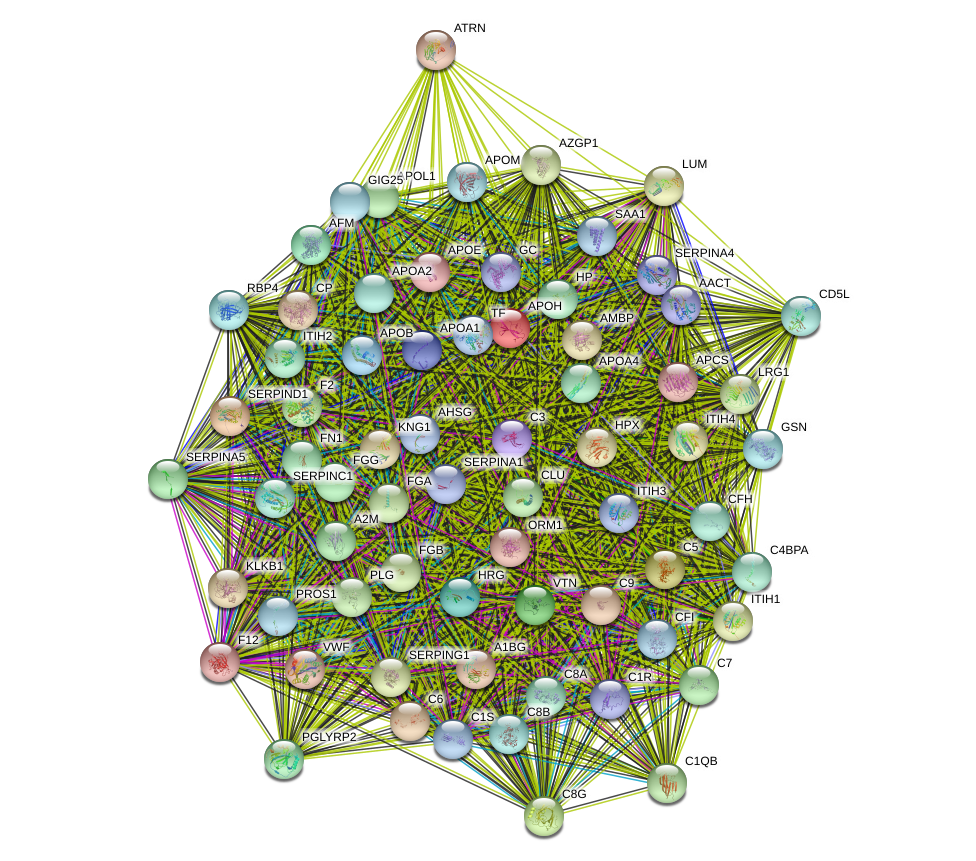
\includegraphics[width=1\linewidth]{figures/openms_protein_quantification/stringdb_plots/acute_c_improvers_vs_nonimprovers_run1_2021-03-23} \caption{The interaction network of differentially abundant proteins found in plasma 2-weeks post-injury, between AIS C patients who experienced an AIS grade conversion and those who did not. The coloured ``halo'' denotes fold change whereby green indicates that protein is less abundant and red indicates greater abundance. Edges represent protein-protein associations; these are known interactions from: curated databases 
\includegraphics[width=0.08\textwidth,height=0.02\textheight]{Images/stringdb_curated_db.png} and those that are experimentally determined 
\includegraphics[width=0.08\textwidth,height=0.02\textheight]{Images/stringdb_experimentally_determined.png}. Predicted interactions from: gene co-occurence 
\includegraphics[width=0.08\textwidth,height=0.02\textheight]{Images/stringdb_gene_co-occurrence.png}; gene fusions 
\includegraphics[width=0.08\textwidth,height=0.02\textheight]{Images/stringdb_gene_fusions.png}; gene neighbourhood 
\includegraphics[width=0.08\textwidth,height=0.02\textheight]{Images/stringdb_gene_neighbour.png}. Others are from gene co-expression 
\includegraphics[width=0.08\textwidth,height=0.02\textheight]{Images/stringdb_co-expression.png}; text-mining 
\includegraphics[width=0.08\textwidth,height=0.02\textheight]{Images/stringdb_text_mining.png} and protein homology 
\includegraphics[width=0.08\textwidth,height=0.02\textheight]{Images/stringdb_protein-homology.png}.}\label{fig:openms-stringdb-acute-c-imp-vs-non}
\end{figure}



\begin{figure}
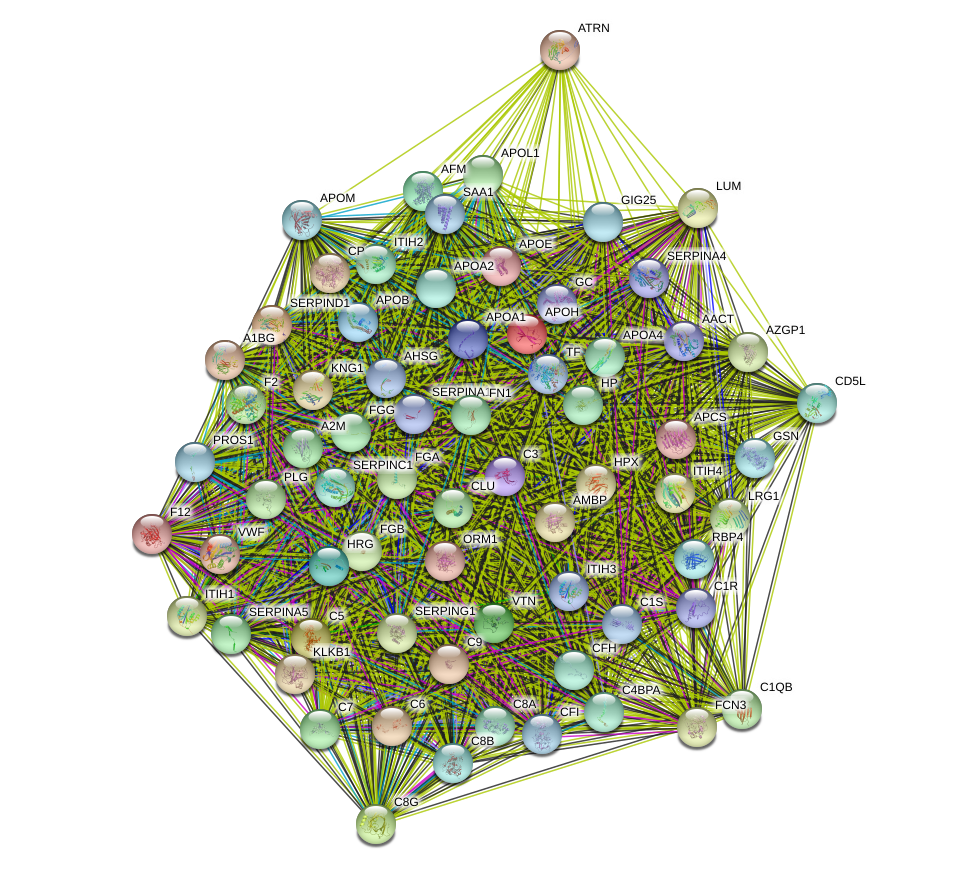
\includegraphics[width=1\linewidth]{figures/openms_protein_quantification/stringdb_plots/subacute_c_improvers_vs_nonimprovers_run1_2021-03-23} \caption{Interaction network of differentially abundant proteins from plasma 3-months post-injury, between AIS C patients who experienced an AIS grade conversion and those who did not. The coloured ``halo'' denotes fold change whereby green indicates that protein is less abundant and red that there is greater abundance. Edges represent protein-protein associations; these are known interactions from: curated databases 
\includegraphics[width=0.08\textwidth,height=0.02\textheight]{Images/stringdb_curated_db.png} and those that are experimentally determined 
\includegraphics[width=0.08\textwidth,height=0.02\textheight]{Images/stringdb_experimentally_determined.png}. Predicted interactions from: gene co-occurence 
\includegraphics[width=0.08\textwidth,height=0.02\textheight]{Images/stringdb_gene_co-occurrence.png}; gene fusions 
\includegraphics[width=0.08\textwidth,height=0.02\textheight]{Images/stringdb_gene_fusions.png}; gene neighbourhood 
\includegraphics[width=0.08\textwidth,height=0.02\textheight]{Images/stringdb_gene_neighbour.png}. Others are from gene co-expression 
\includegraphics[width=0.08\textwidth,height=0.02\textheight]{Images/stringdb_co-expression.png}; text-mining 
\includegraphics[width=0.08\textwidth,height=0.02\textheight]{Images/stringdb_text_mining.png} and protein homology 
\includegraphics[width=0.08\textwidth,height=0.02\textheight]{Images/stringdb_protein-homology.png}.}\label{fig:openms-stringdb-sub-cs}
\end{figure}

\hypertarget{heatmaps-chap3}{%
\subsubsection{Heatmaps}\label{heatmaps-chap3}}

The majority of the pathways associated with the proteins identified by these iTRAQ experiments are related to the complement cascade and clotting via platelets (Figure \ref{fig:openms-hmap-acute-c-1}, \ref{fig:openms-hmap-subacute-c-1}, \ref{fig:openms-hmap-acute-sacute-imp-c-1}, \ref{fig:openms-hmap-acute-sacute-nonimp-c-1}, \ref{fig:openms-hmap-acute-c-2}, \ref{fig:openms-hmap-acute-a-d-2}, \ref{fig:openms-hmap-acute-imp-c-d-2}, \ref{fig:openms-hmap-acute-imp-c-a-2}, \ref{fig:openms-hmap-acute-nonimp-c-a-2}, \ref{fig:openms-hmap-acute-nonimp-c-d-2}).
There are also several pathways implicated in metabolic processes, particularly with apolipoproteins and retinoids.

Please see appendix section \ref{appen-itraq-hmap} for additional plots.

\begin{SidewaysFigure}



\begin{figure}

{\centering \includegraphics{proteomic_paper_2020-02-11_files/figure-latex/openms-hmap-acute-c-1-1} 

}

\caption{Heatmap denoting the log$_2$ fold change of proteins in plasma collected 2-weeks post-injury, and the biological pathways these proteins are associated with on Reactome. This compares AIS C SCI patients who experienced an AIS grade improvement and those who did not.}\label{fig:openms-hmap-acute-c-1}
\end{figure}

\end{SidewaysFigure}
\begin{SidewaysFigure}



\begin{figure}

{\centering \includegraphics{proteomic_paper_2020-02-11_files/figure-latex/openms-hmap-subacute-c-1-1} 

}

\caption{Heatmap denoting the log$_2$ fold change of proteins in plasma collected 3-months post-injury, and the biological pathways these proteins are associated with on Reactome. This compares AIS C SCI patients who experienced an AIS grade improvement and those who did not.}\label{fig:openms-hmap-subacute-c-1}
\end{figure}

\end{SidewaysFigure}
\clearpage

\hypertarget{cnetplot-chap3}{%
\subsubsection{Cnetplots}\label{cnetplot-chap3}}

Similar to the heatmaps, network plots highlight the majority of proteins are associated with the complement cascade and pathways linked to platelets (Figure \ref{fig:openms-cnetp-acute-c-1}, \ref{fig:openms-cnetp-subacute-c-1}, \ref{fig:openms-cnetp-acute-sacute-imp-c-1}, \ref{fig:openms-cnetp-acute-sacute-nonimp-c-1}, \ref{fig:openms-cnetp-acute-c-2}, \ref{fig:openms-cnetp-acute-a-d-2}, \ref{fig:openms-cnetp-acute-imp-c-d-2}, \ref{fig:openms-cnetp-acute-imp-c-a-2}, \ref{fig:openms-cnetp-acute-nonimp-c-a-2}, \ref{fig:openms-cnetp-acute-nonimp-c-d-2}).
Several proteins are also associated with the regulation of insulin-like growth factor.

Please see appendix section \ref{appen-itraq-cnet} for additional plots.

\begin{SidewaysFigure}



\begin{figure}

{\centering \includegraphics{proteomic_paper_2020-02-11_files/figure-latex/openms-cnetp-acute-c-1-1} 

}

\caption{Network plot denoting the log$_2$ fold change of proteins in plasma collected 2-weeks post-injury, and the biological pathways these proteins are associated with on Reactome. This compares AIS C SCI patients who experienced an AIS grade improvement and those who did not.}\label{fig:openms-cnetp-acute-c-1}
\end{figure}

\end{SidewaysFigure}
\begin{SidewaysFigure}



\begin{figure}

{\centering \includegraphics{proteomic_paper_2020-02-11_files/figure-latex/openms-cnetp-subacute-c-1-1} 

}

\caption{Network plot denoting the log$_2$ fold change of proteins in plasma collected 3-months post-injury, and the biological pathways these proteins are associated with on Reactome. This compares AIS C SCI patients who experienced an AIS grade improvement and those who did not.}\label{fig:openms-cnetp-subacute-c-1}
\end{figure}

\end{SidewaysFigure}

\clearpage

\hypertarget{elisas}{%
\subsubsection{ELISAs}\label{elisas}}

No statistically significant difference between groups for A2M abundance in plasma via DuoSet\&reg ELISAs, though there were outliers in the AIS A and D groups, and particularly in the AIS C patients at 3-months who did not experience an AIS grade conversion (Figure \ref{fig:elisa-sig-plots1}).
A significant difference was found between AIS C non-improvers at 2-weeks and AIS D for SAA1, with outliers in AIS C non-improvers at 2-weeks, and both AIS C improvers and non-improvers at 3-months post-injury (Figure \ref{fig:elisa-sig-plots2}).
For ApoA1 plasma abundance estimated via Quantikine\&reg ELISAs, statistically significant differences were found between AIS C improvers at 2-weeks and both AIS C improvers and non-improvers at 3-months, AIS C 3-month improvers and AIS A and D, and AIS C 3-month non-improvers and AIS A and D (Figure \ref{fig:elisa-sig-plots3}).
A statistically significant difference was also found between AIS C improvers and non-improvers at 2-weeks post-injury for RBP4 (Figure \ref{fig:elisa-sig-plots4}).

\clearpage



\begin{figure}
\centering
\includegraphics{proteomic_paper_2020-02-11_files/figure-latex/elisa-sig-plots1-1.pdf}
\caption{\label{fig:elisa-sig-plots1}Normalised estimated concentration of \(\alpha\)-2-macroglobulin. Estimates were calculated from the optical density of a standard curve produced via a DuoSet\&reg ELISA. Plasma from each patient that made up the pooled iTRAQ samples was assayed and pairwise t-tests with bonferroni adjusted P-values were preformed to assess differential abundance.}
\end{figure}



\begin{figure}
\centering
\includegraphics{proteomic_paper_2020-02-11_files/figure-latex/elisa-sig-plots2-1.pdf}
\caption{\label{fig:elisa-sig-plots2}Normalised estimated concentration of serum amyloid A1. Estimates were calculated from the optical density of a standard curve produced via a DuoSet\&reg ELISA. Plasma from each patient that made up the pooled iTRAQ samples was assayed and pairwise t-tests with bonferroni adjusted P-values were preformed to assess differential abundance.}
\end{figure}



\begin{figure}
\centering
\includegraphics{proteomic_paper_2020-02-11_files/figure-latex/elisa-sig-plots3-1.pdf}
\caption{\label{fig:elisa-sig-plots3}Normalised estimated concentration of apolipoprotein A1. Estimates were calculated from the optical density of a standard curve produced via a Quantikine\&reg ELISA. Plasma from each patient that made up the pooled iTRAQ samples was assayed and pairwise t-tests with bonferroni adjusted P-values were preformed to assess differential abundance.}
\end{figure}



\begin{figure}
\centering
\includegraphics{proteomic_paper_2020-02-11_files/figure-latex/elisa-sig-plots4-1.pdf}
\caption{\label{fig:elisa-sig-plots4}Normalised estimated concentration of retinol binding protein 4. Estimates were calculated from the optical density of a standard curve produced via a DuoSet\&reg ELISA. Plasma from each patient that made up the pooled iTRAQ samples was assayed and pairwise t-tests with bonferroni adjusted P-values were preformed to assess differential abundance.}
\end{figure}

\hypertarget{kegg-chap3}{%
\subsubsection{Pathway analysis}\label{kegg-chap3}}

Pathway analysis via the \texttt{pathview} R package returned the complement and coagulation cascade to be on the sole significant KEGG pathway to derive from the OpenMS analysed data.
The majority of the proteins present in this pathway were less abundant in the 2-week post-injury plasma of AIS C patients who experienced an AIS grade conversion and those who did not (Figure \ref{fig:kegg-complement}.



\begin{figure}

{\centering 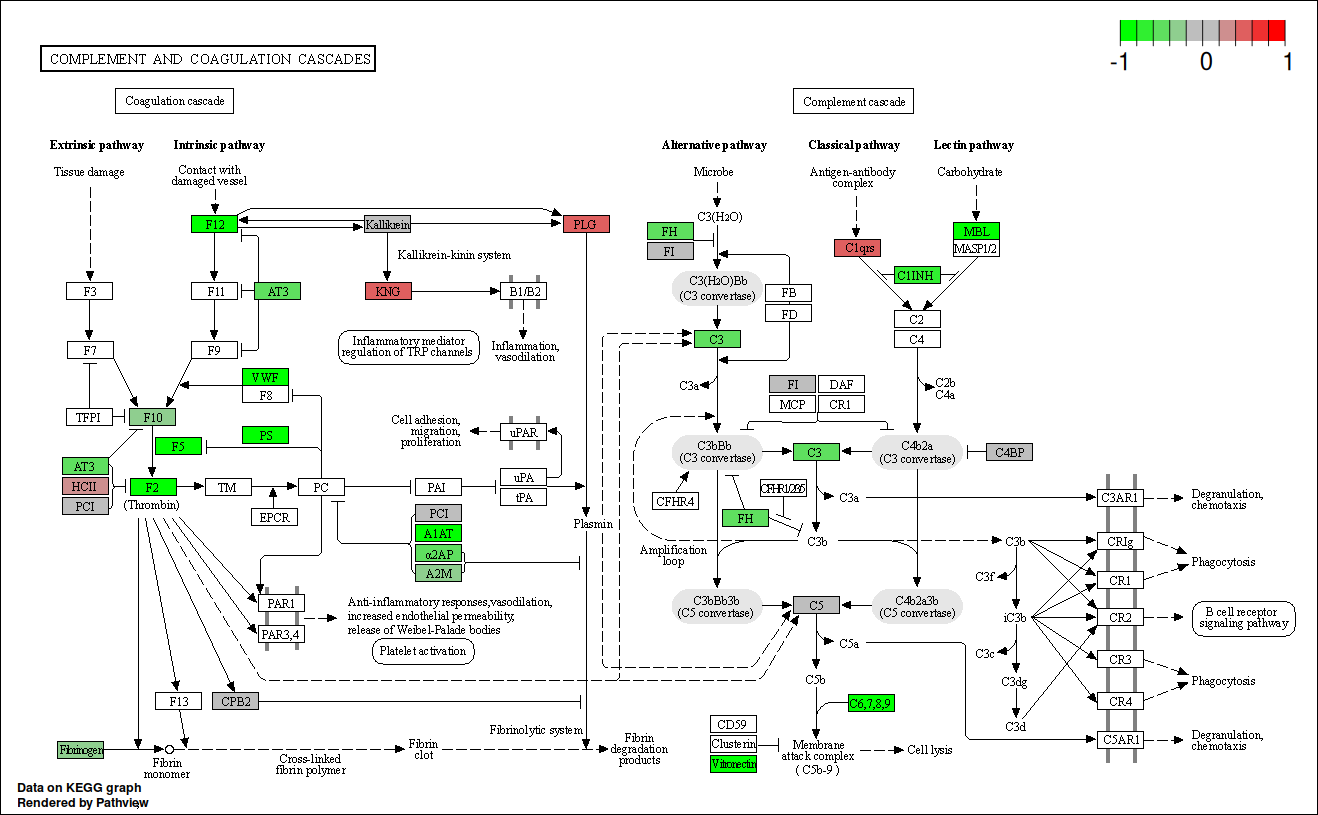
\includegraphics[width=18.31in]{figures/kegg_pathways/hsa04610_pathview} 

}

\caption{KEGG complement cascade pathway annotated with log\(_2\) fold change of proteins in plasma collected 2-weeks post-injury. This compares AIS C SCI patients who experienced an AIS grade improvement and those who did not.}\label{fig:kegg-complement}
\end{figure}

\clearpage

\hypertarget{chap-4-results}{%
\subsection{Label-free results}\label{chap-4-results}}

In the interest of brevity, only the plots of acute and subactue AIS C improvers VS non-improvers are included here, please see the appendix for the other comparisons (section \ref{appen-labelfree}).

The data processed by \texttt{MSstats} was filtered to proteins with a adjusted P-value of \textless{} 0.05 and a log\(_2\) FC of \textgreater{} \(\pm1.2\).
The total number of significant proteins is \texttt{nrow(foldchange\_df)}.

\hypertarget{volcano-plots}{%
\subsubsection{Volcano plots}\label{volcano-plots}}

The mean number of down-regulated and up-regulated significant proteins in each group is 10.5714286, and 6.7857143.
Between AIS C improvers and non-improvers, 8 and 4 proteins were up- and down-regulated acutely, whereas 6 and 6 were up- and down-regulated subacutely (Figures \ref{fig:volc-plot-c-imp-vs-nonimp} and \ref{fig:volc-plot-subacute-c-imp-vs-nonimp}).
Longitudinally, AIS C acute improvers had 10 up-regulated and 7 down-regulated proteins relative to subacute improvers, while for non-improvers 6 and 12 were up- and down-regulated respectively (Figures \ref{fig:volc-plot-acute-c-imp-vs-subacute-imp} and \ref{fig:volc-plot-acute-c-nonimp-vs-subacute-nonimp}).

Please see appendix section \ref{appen-labelfree-volc} for additional plots.

\clearpage



\begin{figure}
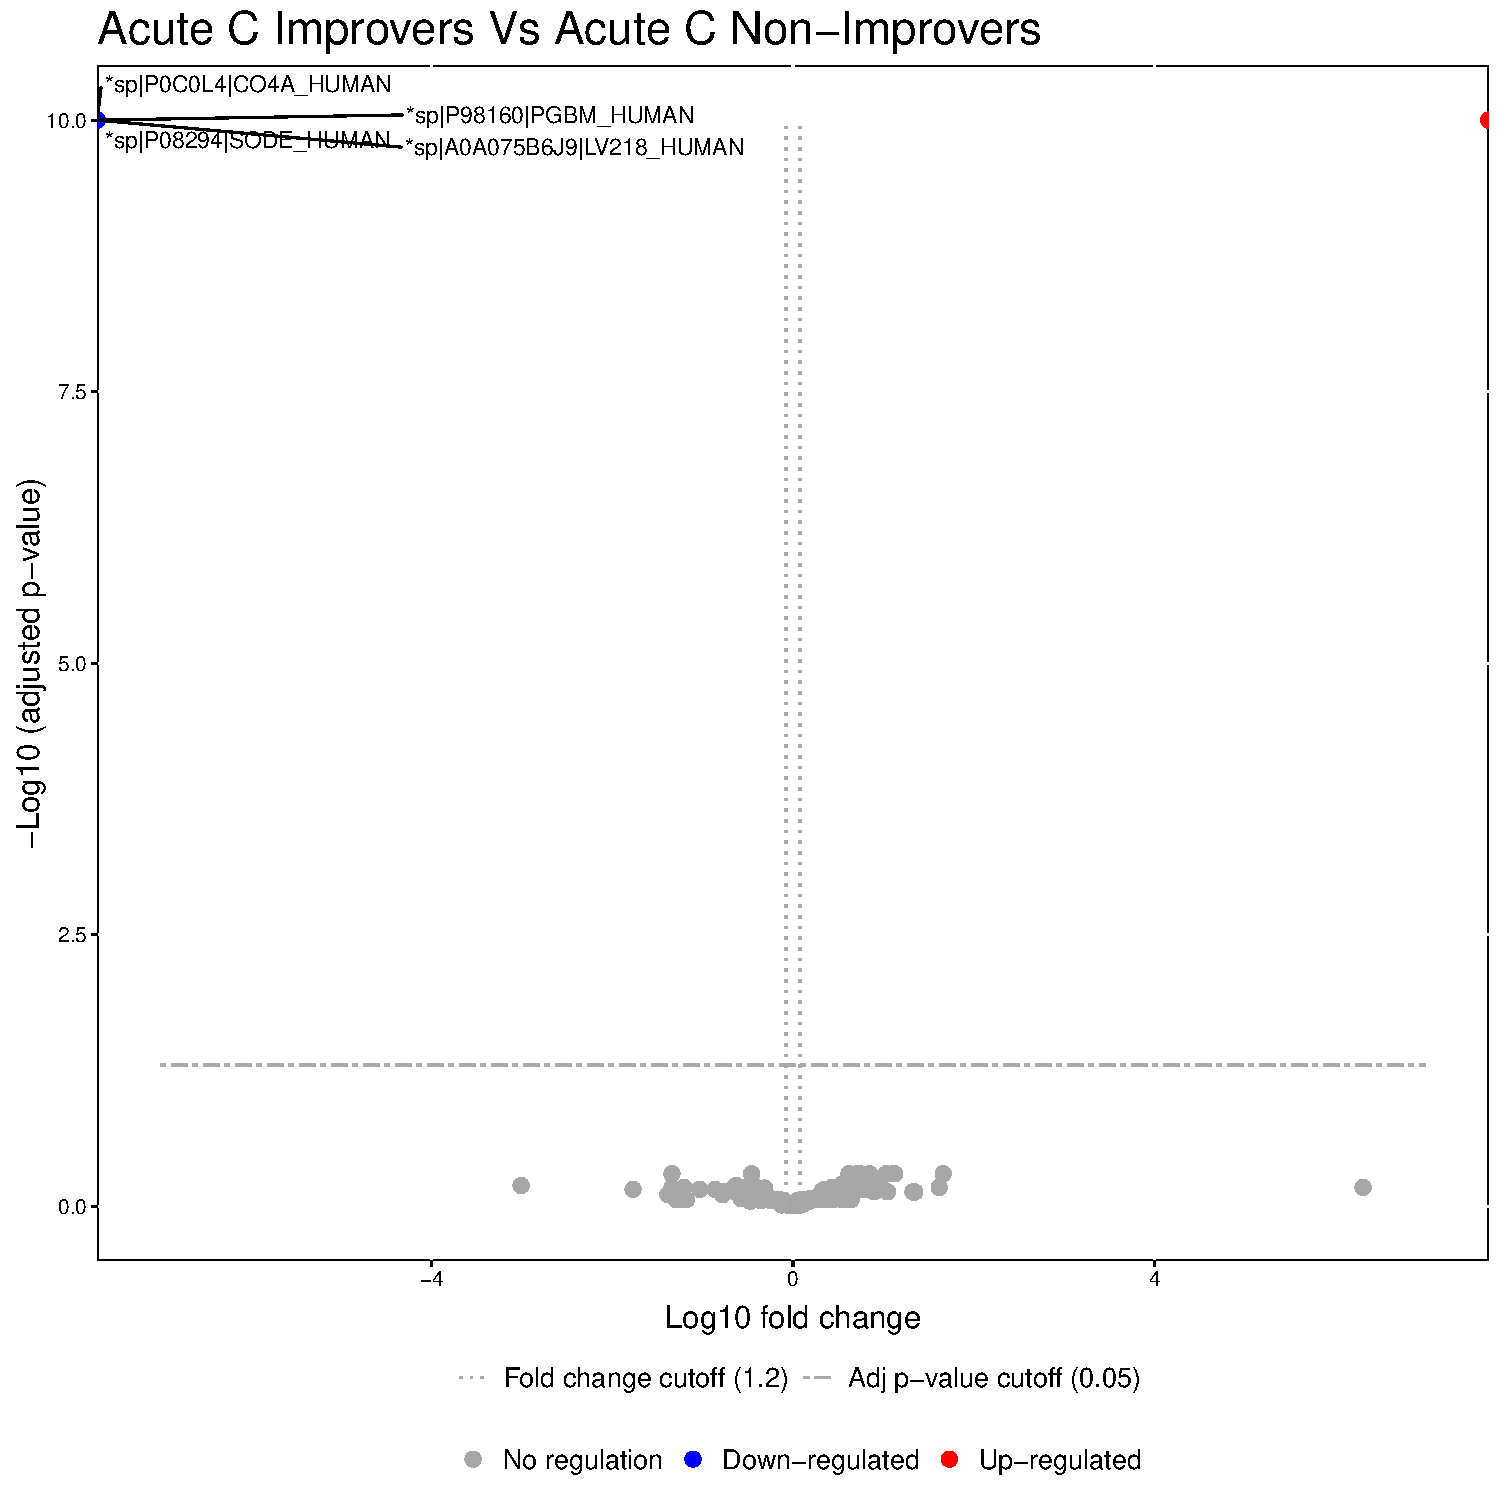
\includegraphics[width=1\linewidth]{figures/openms_protein_quantification/label_free/openms_volcano_plot_2021-08-10_0008} \caption{Volcano plot of log\(_10\) fold change and log\(_10\) adjusted p-value for plasma proteins from 2-weeks post-injury between AIS C patients who experienced an AIS grade conversion and those who did not. Proteins with a fold changes beyond \(\pm 1.2\) and an adjusted p-value less than 0.05 are labelled.}\label{fig:volc-plot-c-imp-vs-nonimp}
\end{figure}



\begin{figure}
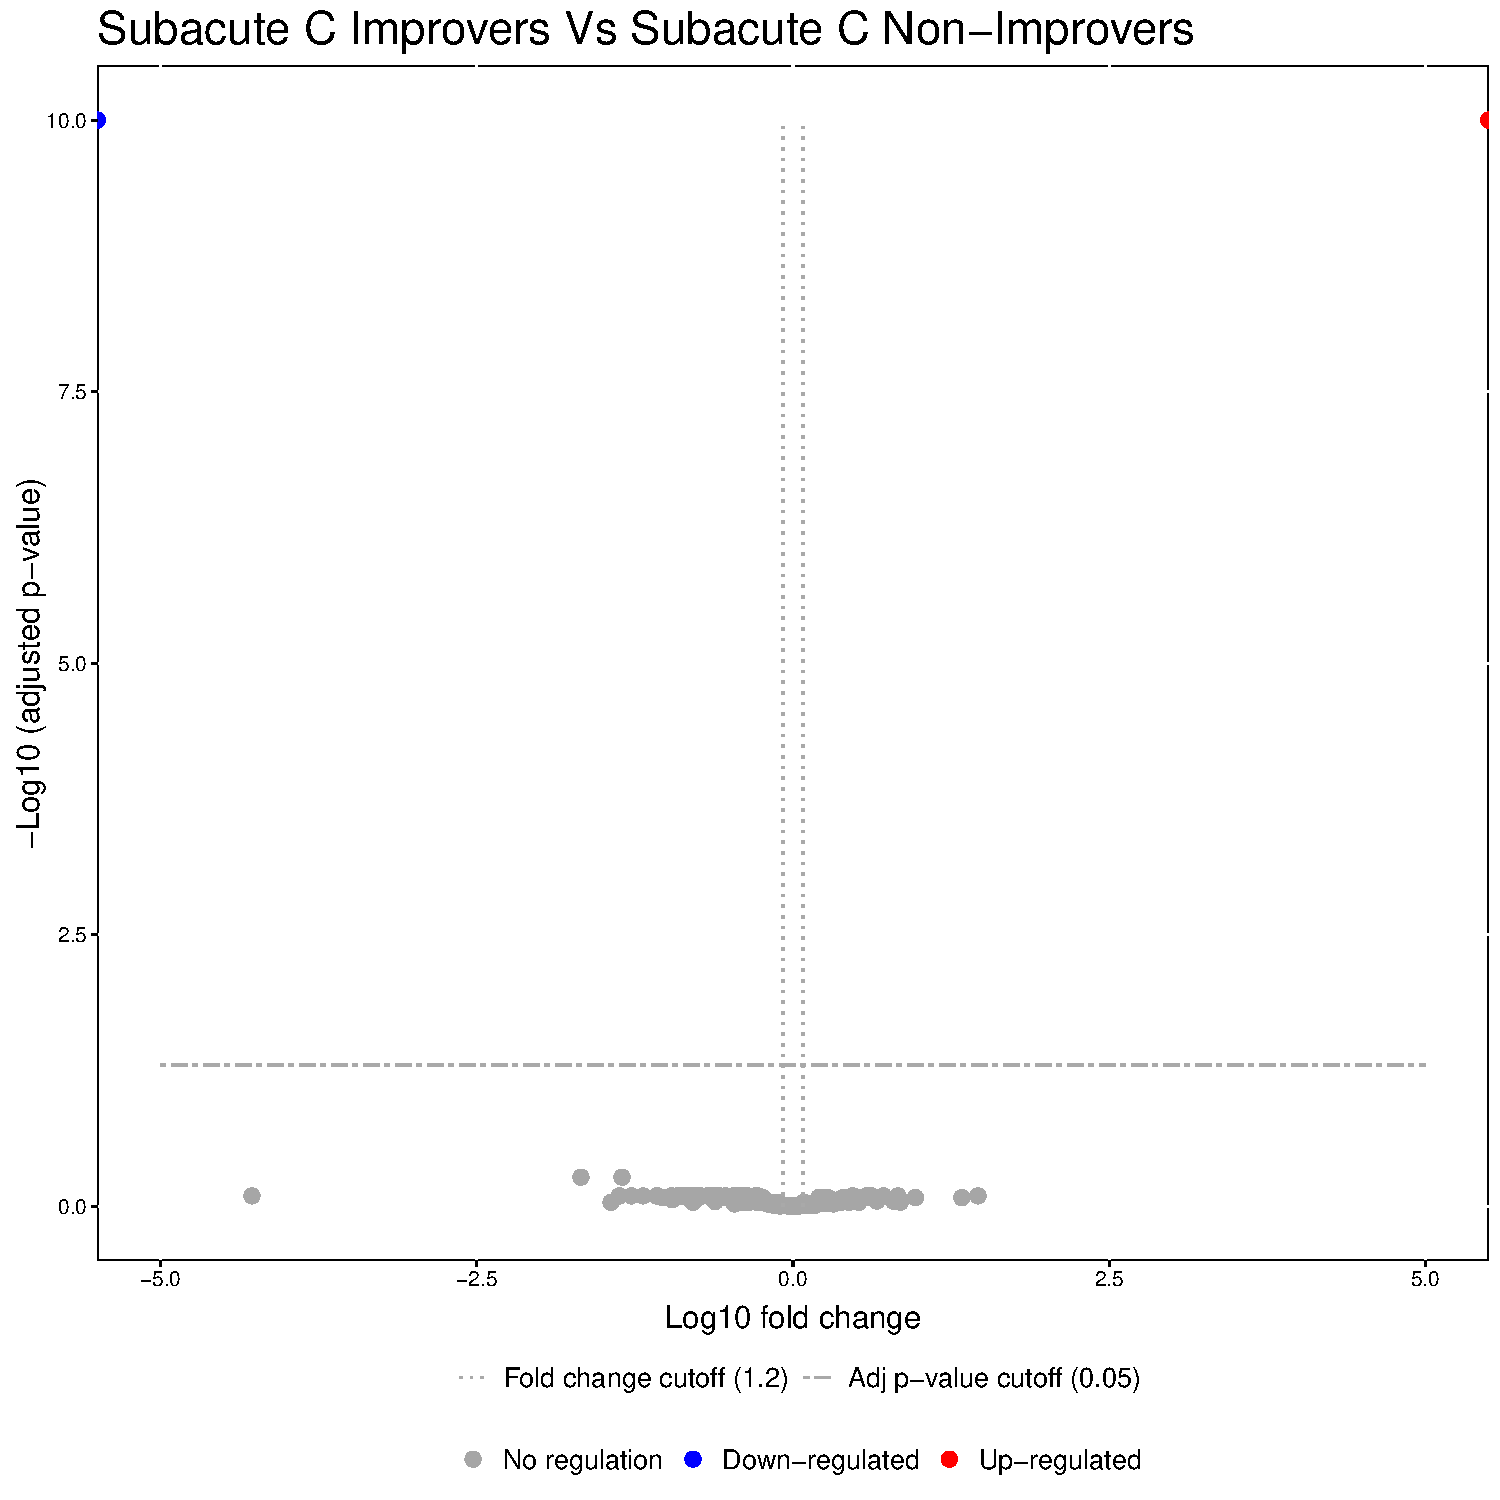
\includegraphics[width=1\linewidth]{figures/openms_protein_quantification/label_free/openms_volcano_plot_2021-08-10_0026} \caption{Volcano plot of log\(_10\) fold change and log\(_10\) adjusted p-value for plasma proteins from 3-months post-injury between AIS C patients who experienced an AIS grade conversion and those who did not. Proteins with a fold changes beyond \(\pm 1.2\) and an adjusted p-value less than 0.05 are labelled.}\label{fig:volc-plot-subacute-c-imp-vs-nonimp}
\end{figure}

\hypertarget{stringdb-network-plots-1}{%
\subsubsection{STRINGdb network plots}\label{stringdb-network-plots-1}}

Network interaction plots generated of the significant proteins via \texttt{STRINGdb} revealed that all groups contained similarly smaller networks, with many proteins with no know interactions in the STRING database (Figures \ref{fig:openms-stringdb-chap4-acute-c-imp-vs-nonimp}, \ref{fig:openms-stringdb-chap4-sub-cs}, \ref{fig:openms-stringdb-chap4-acute-sub-c-imp}, \ref{fig:openms-stringdb-chap4-acute-sub-c-nonimp}, \ref{fig:openms-stringdb-chap4-a-vs-d}, \ref{fig:openms-stringdb-chap4-c-vs-d}, \ref{fig:openms-stringdb-chap4-c-vs-a}, \ref{fig:openms-stringdb-chap4-c-nonimp-vs-a}, \ref{fig:openms-stringdb-chap4-c-nonimp-vs-d}.

Clustering of these plots furhter highlights the smaller groups of interacting proteins, many of which are linear networks of proteins interacting in a chain (Figures \ref{fig:openms-stringdb-cluster-chap4-acute-c-imp-vs-nonimp}, \ref{fig:openms-stringdb-cluster-chap4-sub-c-imp-vs-nonimp}, \ref{fig:openms-stringdb-cluster-chap4-acute-sub-c-imp}, \ref{fig:openms-stringdb-cluster-chap4-acute-sub-c-nonimp}, \ref{fig:openms-stringdb-cluster-chap4-a-vs-d}, \ref{fig:openms-stringdb-cluster-chap4-c-vs-a}, \ref{fig:openms-stringdb-cluster-chap4-c-vs-d}, \ref{fig:openms-stringdb-cluster-chap4-c-nonimp-vs-a}, \ref{fig:openms-stringdb-cluster-chap4-c-nonimp-vs-d}).
Please note that only clusters containing more than one protein are shown.

Please see appendix section \ref{appen-labelfree-string} for additional plots.



\begin{figure}
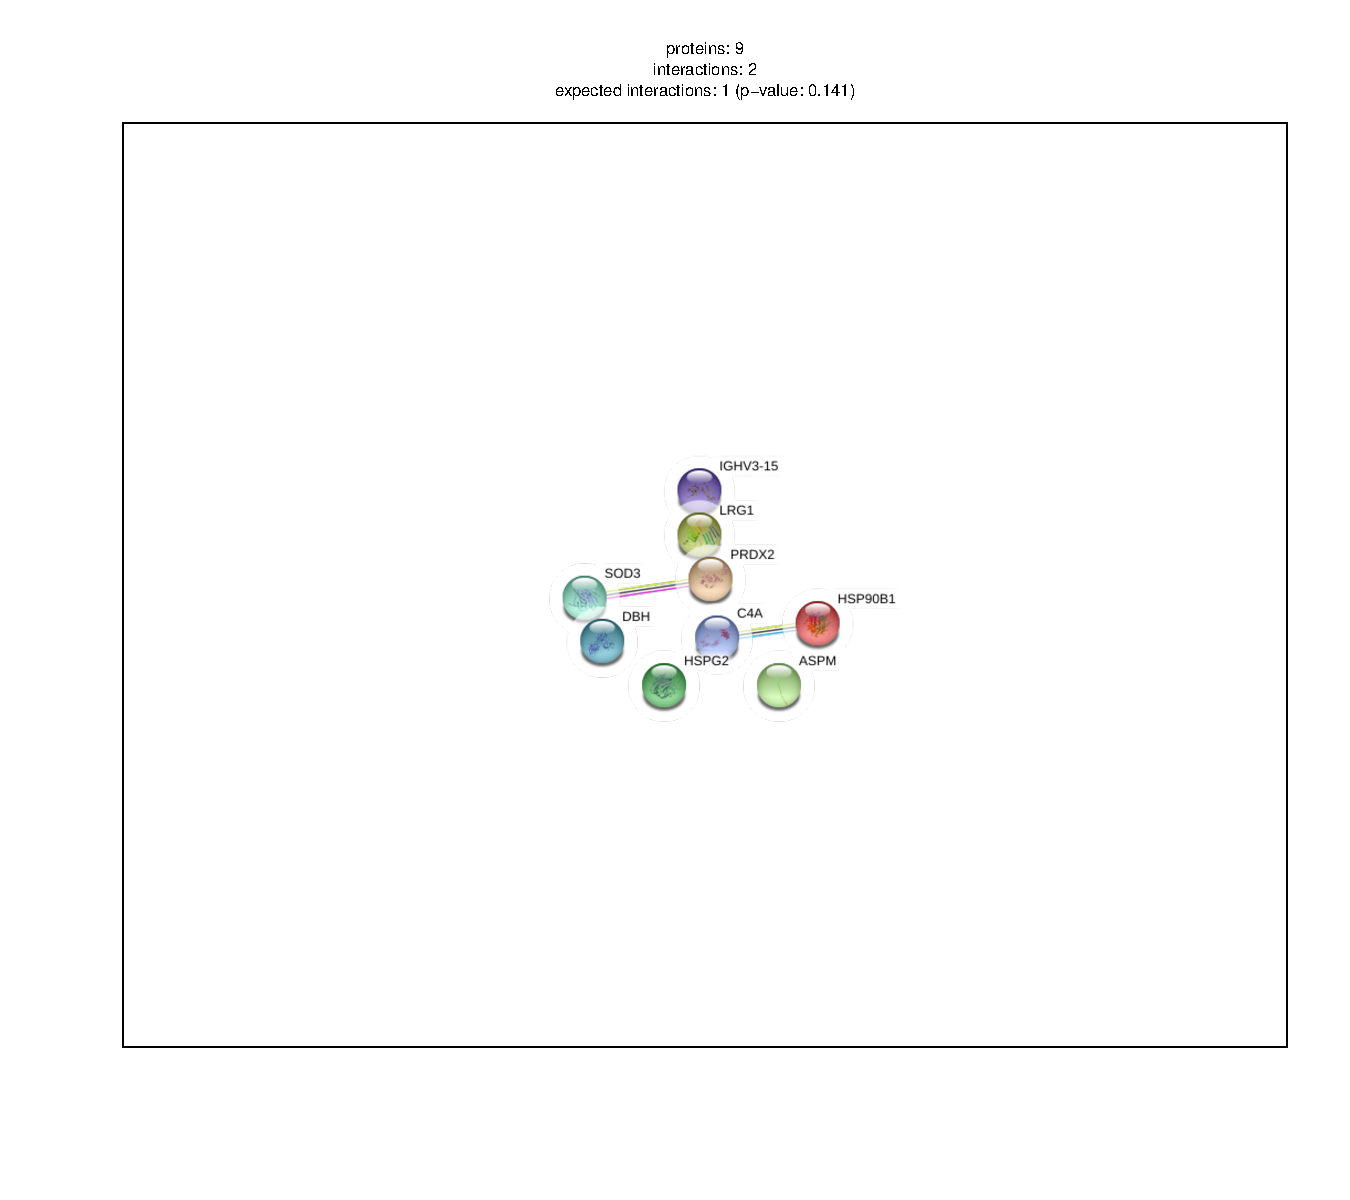
\includegraphics[width=1\linewidth]{figures/openms_protein_quantification/label_free/stringdb_plots/acute_c_imp_vs_acute_c_nonimp_2021-08-06} \caption{The interaction network of differentially abundant proteins found in plasma 2-weeks post-injury, between AIS C patients who experienced an AIS grade conversion and those who did not. The coloured ``halo'' denotes fold change whereby green indicates that protein is less abundant and red indicates greater abundance. Edges represent protein-protein associations; these are known interactions from: curated databases 
\includegraphics[width=0.08\textwidth,height=0.02\textheight]{Images/stringdb_curated_db.png} and those that are experimentally determined 
\includegraphics[width=0.08\textwidth,height=0.02\textheight]{Images/stringdb_experimentally_determined.png}. Predicted interactions from: gene co-occurence 
\includegraphics[width=0.08\textwidth,height=0.02\textheight]{Images/stringdb_gene_co-occurrence.png}; gene fusions 
\includegraphics[width=0.08\textwidth,height=0.02\textheight]{Images/stringdb_gene_fusions.png}; gene neighbourhood 
\includegraphics[width=0.08\textwidth,height=0.02\textheight]{Images/stringdb_gene_neighbour.png}. Others are from gene co-expression 
\includegraphics[width=0.08\textwidth,height=0.02\textheight]{Images/stringdb_co-expression.png}; text-mining 
\includegraphics[width=0.08\textwidth,height=0.02\textheight]{Images/stringdb_text_mining.png} and protein homology 
\includegraphics[width=0.08\textwidth,height=0.02\textheight]{Images/stringdb_protein-homology.png}.}\label{fig:openms-stringdb-chap4-acute-c-imp-vs-nonimp}
\end{figure}



\begin{figure}
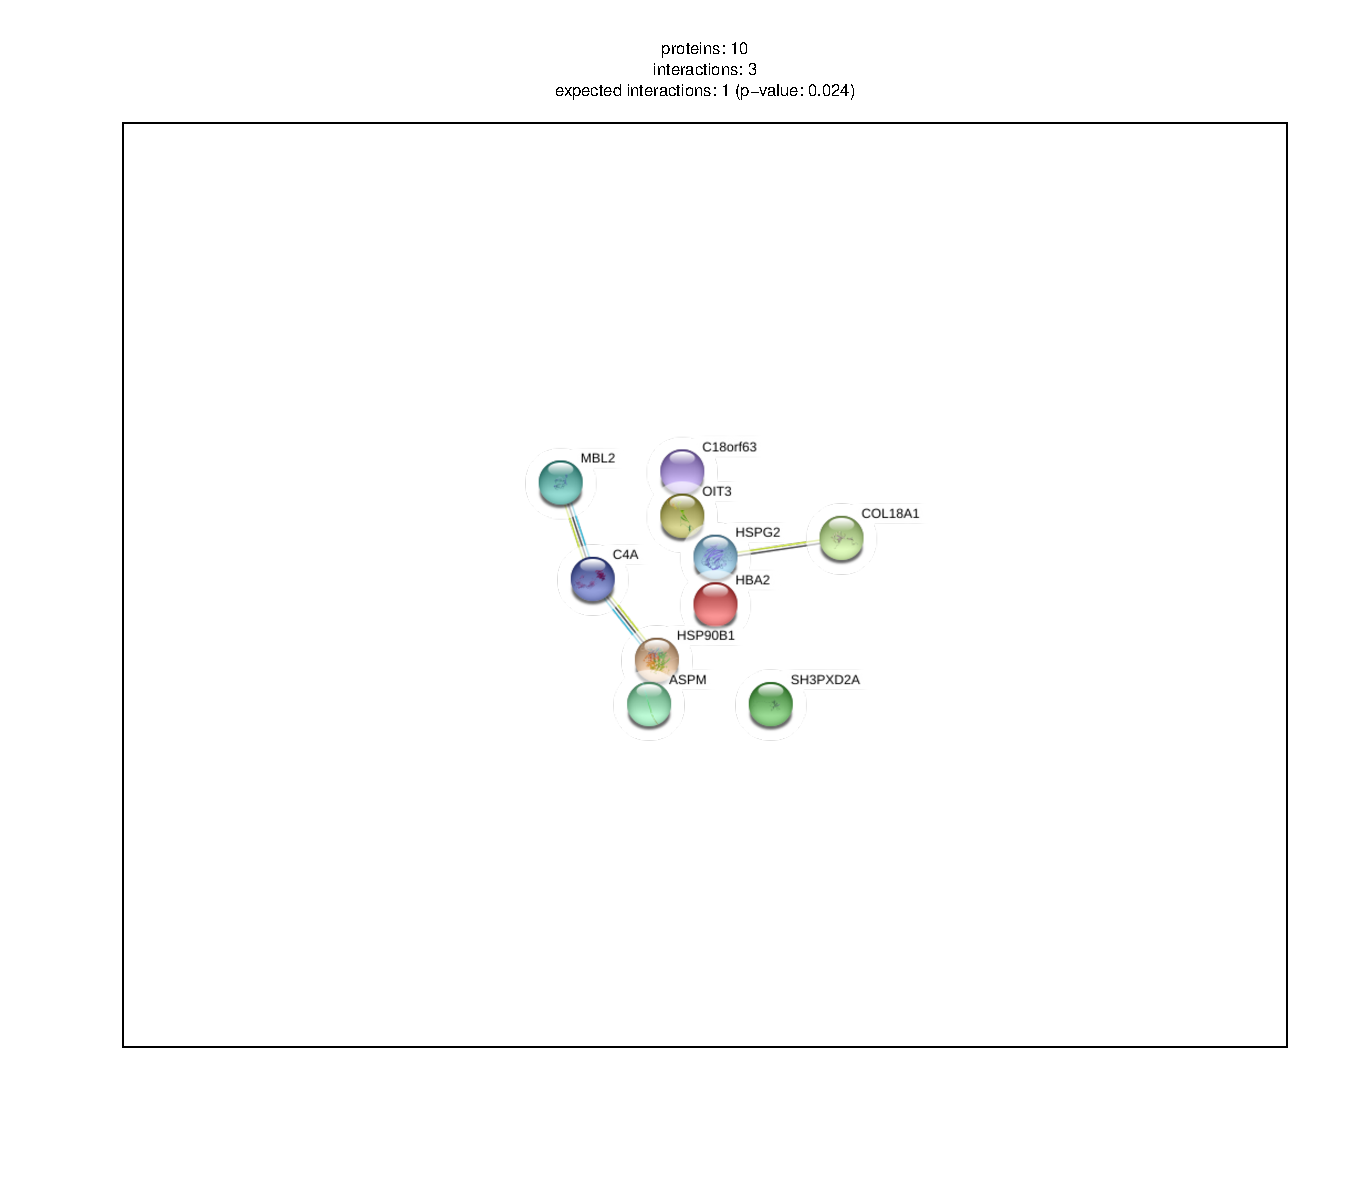
\includegraphics[width=1\linewidth]{figures/openms_protein_quantification/label_free/stringdb_plots/subacute_c_imp_vs_subacute_c_nonimp_2021-08-06} \caption{Interaction network of differentially abundant proteins from plasma 3-months post-injury, between AIS C patients who experienced an AIS grade conversion and those who did not. The coloured ``halo'' denotes fold change whereby green indicates that protein is less abundant and red that there is greater abundance. Edges represent protein-protein associations; these are known interactions from: curated databases 
\includegraphics[width=0.08\textwidth,height=0.02\textheight]{Images/stringdb_curated_db.png} and those that are experimentally determined 
\includegraphics[width=0.08\textwidth,height=0.02\textheight]{Images/stringdb_experimentally_determined.png}. Predicted interactions from: gene co-occurence 
\includegraphics[width=0.08\textwidth,height=0.02\textheight]{Images/stringdb_gene_co-occurrence.png}; gene fusions 
\includegraphics[width=0.08\textwidth,height=0.02\textheight]{Images/stringdb_gene_fusions.png}; gene neighbourhood 
\includegraphics[width=0.08\textwidth,height=0.02\textheight]{Images/stringdb_gene_neighbour.png}. Others are from gene co-expression 
\includegraphics[width=0.08\textwidth,height=0.02\textheight]{Images/stringdb_co-expression.png}; text-mining 
\includegraphics[width=0.08\textwidth,height=0.02\textheight]{Images/stringdb_text_mining.png} and protein homology \includegraphics[width=0.08\textwidth,height=0.02\textheight]{Images/stringdb_protein-homology.png}.}\label{fig:openms-stringdb-chap4-sub-cs}
\end{figure}

\hypertarget{heatmaps}{%
\subsubsection{Heatmaps}\label{heatmaps}}

Similarly to the iTRAQ data (\ref{heatmaps-chap3}), many of the Reactome pathways are associated with the complement cascade, platelets and clotting (Figures \ref{fig:openms-chap4-hmap-acute-c-1}, \ref{fig:openms-chap4-hmap-subacute-c-1}, \ref{fig:openms-chap4-hmap-acute-sacute-imp-c-1}, \ref{fig:openms-chap4-hmap-acute-sacute-nonimp-c-1}, \ref{fig:openms-chap4-hmap-acute-a-d-2}, \ref{fig:openms-chap4-hmap-acute-imp-c-d-2}, \ref{fig:openms-chap4-hmap-acute-imp-c-a-2}, \ref{fig:openms-chap4-hmap-acute-nonimp-c-a-2}, \ref{fig:openms-chap4-hmap-acute-nonimp-c-d-2}).

Please see appendix section \ref{appen-labelfree-hmap} for additional plots.

\begin{SidewaysFigure}



\begin{figure}

{\centering \includegraphics{proteomic_paper_2020-02-11_files/figure-latex/openms-chap4-hmap-acute-c-1-1} 

}

\caption{Heatmap denoting the log$_2$ fold change of proteins in plasma collected 2-weeks post-injury, and the biological pathways these proteins are associated with on Reactome. This compares AIS C SCI patients who experienced an AIS grade improvement and those who did not. Grey blocks denote proteins not present in the comparison.}\label{fig:openms-chap4-hmap-acute-c-1}
\end{figure}

\end{SidewaysFigure}
\begin{SidewaysFigure}



\begin{figure}

{\centering \includegraphics{proteomic_paper_2020-02-11_files/figure-latex/openms-chap4-hmap-subacute-c-1-1} 

}

\caption{Heatmap denoting the log$_2$ fold change of proteins in plasma collected 3-months post-injury, and the biological pathways these proteins are associated with on Reactome. This compares AIS C SCI patients who experienced an AIS grade improvement and those who did not. Grey blocks denote proteins not present in the comparison.}\label{fig:openms-chap4-hmap-subacute-c-1}
\end{figure}

\end{SidewaysFigure}
\clearpage

\hypertarget{cnetplots}{%
\subsubsection{Cnetplots}\label{cnetplots}}

Similarly to the heatmaps and the iTRAQ data (\ref{cnetplot-chap3}),network plots highlight the majority of proteins are associated with the complement cascade and pathways linked to platelets (Figures \ref{fig:openms-chap4-cnetp-acute-c-1}, \ref{fig:openms-chap4-cnetp-subacute-c-1}, \ref{fig:openms-chap4-cnetp-acute-sacute-imp-c-1}, \ref{fig:openms-chap4-cnetp-acute-sacute-nonimp-c-1}, \ref{fig:openms-chap4-cnetp-acute-a-d-2}, \ref{fig:openms-chap4-cnetp-acute-imp-c-d-2}, \ref{fig:openms-chap4-cnetp-acute-imp-c-a-2}, \ref{fig:openms-chap4-cnetp-acute-nonimp-c-a-2}, \ref{fig:openms-chap4-cnetp-acute-nonimp-c-d-2}).

Please see appendix section \ref{appen-labelfree-cnet} for additional plots.

\begin{SidewaysFigure}



\begin{figure}

{\centering \includegraphics{proteomic_paper_2020-02-11_files/figure-latex/openms-chap4-cnetp-acute-c-1-1} 

}

\caption{Network plot denoting the log$_2$ fold change of proteins in plasma collected 2-weeks post-injury, and the biological pathways these proteins are associated with on Reactome. This compares AIS C SCI patients who experienced an AIS grade improvement and those who did not.}\label{fig:openms-chap4-cnetp-acute-c-1}
\end{figure}

\end{SidewaysFigure}
\begin{SidewaysFigure}



\begin{figure}

{\centering \includegraphics{proteomic_paper_2020-02-11_files/figure-latex/openms-chap4-cnetp-subacute-c-1-1} 

}

\caption{Network plot denoting the log$_2$ fold change of proteins in plasma collected 3-months post-injury, and the biological pathways these proteins are associated with on Reactome. This compares AIS C SCI patients who experienced an AIS grade improvement and those who did not.}\label{fig:openms-chap4-cnetp-subacute-c-1}
\end{figure}

\end{SidewaysFigure}
\clearpage

\hypertarget{pathway-analysis}{%
\subsubsection{Pathway analysis}\label{pathway-analysis}}

As with the iTRAQ data (section \ref{kegg-chap3}), pathway analysis via the \texttt{pathview} R package returned the complement and coagulation cascade to be on the sole significant KEGG pathway.
The majority of the proteins present in this pathway were less abundant in the 2-week post-injury plasma of AIS C patients who experienced an AIS grade conversion and those who did not, much the same as the iTRAQ data (Figure \ref{fig:kegg-complement-chap4} and section \ref{kegg-chap3}).



\begin{figure}

{\centering \includegraphics[width=18.31in]{figures/kegg_pathways/hsa04610.pathview_label-free} 

}

\caption{KEGG complement cascade pathway annotated with log\(_2\) fold change of proteins in plasma collected 2-weeks post-injury. This compares AIS C SCI patients who experienced an AIS grade improvement and those who did not.}\label{fig:kegg-complement-chap4}
\end{figure}

\hypertarget{comparing-itraq-and-label-free-proteins}{%
\subsubsection{Comparing iTRAQ and label-free proteins}\label{comparing-itraq-and-label-free-proteins}}

A total of 87 and 79 unique proteins were identified across the label-free and iTRAQ experiments respectively, with modest overlap in those identified (Figure \ref{fig:itraq-label-free-venn}).



\begin{figure}

{\centering \includegraphics[width=0.6\linewidth]{proteomic_paper_2020-02-11_files/figure-latex/itraq-label-free-venn-1} 

}

\caption{Venn diagram of the overlap in unique proteins identified from iTRAQ and label-free proteomic experiments analysed via OpenMS.}\label{fig:itraq-label-free-venn}
\end{figure}

\hypertarget{discussion}{%
\section{Discussion}\label{discussion}}

\hypertarget{thesis-itraq-discussion}{%
\subsection{thesis iTRAQ discussion}\label{thesis-itraq-discussion}}

This work builds on the previous chapters (\ref{chap-2-intro}) modelling of routine bloods by analysing the plasma proteome of SCI patients grouped by injury severity and improver status.
In addition to continuing the pursuit of novel biomarkers of SCI, the link between the liver and neurological recovery hinted at in the aforementioned chapter is examined here.

\hypertarget{proteinpilot-and-openms}{%
\subsubsection{ProteinPilot and OpenMS}\label{proteinpilot-and-openms}}

Mass spectrometry is a major technique used in several fields, including metabolomics, lipidomics, interactomics and proteomics, each of which demands a variety of differing approaches to data acquisition and analysis.
Multiple separation methods (liquid chromatography, gas chromatography), fragmentation methods (electron-capture dissociation, electron-transfer dissociation, collision-induced dissociation, etc.) and acquisition strategies (targeted, data-dependent and data-independent) are used in any combination.
With quantification there are different label-free, isotopic or isobaric labelling approaches to employ.
Finally the data analysis may require a database search, as in proteomics and metabolomics, spectral library search or a targeted analysis, depending on the experiment.
This complexity necessitates a multi-interdependent-step workflow tailored to the given experiment.

The manufacturers of mass spectrometers often offer software tailored to their instruments which is often used in the literature.
However, the source code for these software suits is not publicly available, and indeed manufactures often boast of their particular inscrutable proprietary algorithms, often related to peak picking.
This combination of completixy and opacity in analysis methodolotgy can make it extremely difficult to reproducle results from other labs, or even analysis from one's own lab.\textsuperscript{\protect\hyperlink{ref-noauthor_devil_2011}{45}}

To address this issue many open-source (meaning the source code is publicly available) software packages which may perform one or several steps of a complex analysis workflow have been developed.
This issue here is that incorporating multiple software packages together can be both time-consuming and error-prone, and require significant maintenance and documentation to maintain reproducibility.

The OpenMS project aims to address these challenges by providing a flexible software environment, with both pre-assembled workflows that aim to provide best-practices, and allow for more granular control with both command line and Python scripting interfaces.
OpenMS is also integrated with graphical workflow systems such as KNIME and Galaxy, increasing the accessibility of the platform.\textsuperscript{\protect\hyperlink{ref-berthold_knime_2009}{46},\protect\hyperlink{ref-goecks_galaxy_2010}{47}}

Here we used both the vendor provided proprietary ProteinPilot and OpenMS to analysis two 4-plex iTRAQ experiments.
We observe that both approaches produce similar results, with a similar number of total proteins identified, a large degree of overlap in the specific proteins identified, and similar fold changes (Figures \ref{fig:openms-pp-venn} and \ref{fig:openms-pp-updown}).
As the results are similar we choose to focus on the OpenMS results due to aforementioned superior reproducibility.

\hypertarget{proteins-identified}{%
\subsubsection{Proteins identified}\label{proteins-identified}}

A total of 79 proteins were identified across both runs for OpenMS, many of which are related in function. (Figure \ref{fig:openms-pp-venn}).
Here we explore the potential these proteins have a biomarkers of SCI.

\hypertarget{alpha-2-macroglobulin}{%
\paragraph{Alpha-2-macroglobulin}\label{alpha-2-macroglobulin}}

A2M is an inhibitor of an unusually diverse array of proteinases by a unique `trapping' mechanism.
The protein achieves this with a peptide stretch, called the ``bait region'', which contains specific cleavage sites for different proteinases.
When a proteinase cleaves the bait region, a conformational change is induced whereby A2M traps the proteinase.
The entrapped enzyme retains active against low molecular weight substrates, whereas activity against high molecular weight substrates is greatly reduced.
Following cleavage in the bait region, a thioester bond is hydrolysed and mediates the covalent binding of the protein to the proteinase.\textsuperscript{\protect\hyperlink{ref-hall_proteolytic_1981}{48},\protect\hyperlink{ref-sottrup-jensen_primary_1984}{49}}
A2M is unique in it's ability to inhibit virtually any protease regardless of it's specificity, origin or catalytic mechanism.\textsuperscript{\protect\hyperlink{ref-khan_oxidized_2004}{50},\protect\hyperlink{ref-lin_n-glycosylation_2012}{51}}

Alpha macroglobulins are an integral part of innate immunity and thus are evolutionarily conserved.\textsuperscript{\protect\hyperlink{ref-buresova_iram2-macroglobulin_2009}{52}}
Alpha macroglobulins have significant primary sequence homology with complement components C3, C4 and C5.
The A2M-proteinase complex is cleared from circulation primarily by receptors on hepatocytes.\textsuperscript{\protect\hyperlink{ref-bond_incorporation_2007}{53},\protect\hyperlink{ref-travis_human_1983}{54}}
The mammalian receptor for proteinase‐reacted A2M is a low‐density lipoprotein receptor related protein.\textsuperscript{\protect\hyperlink{ref-fujiyoshi_amyloid-_2011}{55}--\protect\hyperlink{ref-wyatt_acute_2013}{57}}

A2Ms definitive function is the delivery of proteinase to an endocytotic proteinase clearance pathway.
A2Ms trap the proteinases released by granulocytes and other cells during inflammation and also regulate the extracellular proteolytic activity resulting from clotting and fibrinolysis.
A2M can also help protect against pathogens as it can trap proteinases from non-human origins as well.
A2M can be recognised and phagocytosed by macrophages and hepatocytes, and it has been proposed to aid in the clearance of defensins and other peptide mediators in inflamed tissues, thus contributing to the regulation and containment of inflammation.\textsuperscript{\protect\hyperlink{ref-rehman_alpha-2-macroglobulin_2013}{58}}

Myelin basic protein is released into the circulation following traumatic injury and A2M has been seen to be the only major myelin basic protein-binding protein in human plasma, suggesting A2M protects the immunogenic protein from degradation by proteases and help in its clearance from circulation.\textsuperscript{\protect\hyperlink{ref-gunnarsson_binding_1998}{59}}
A study looking at male infertility after SCI with proteomics found A2M to be elevated approximately 3-fold in the sperm plasma of SCI patients relative to normal controls.\textsuperscript{\protect\hyperlink{ref-silva_towards_2016}{60}}

We observe A2M to be less abundant in AIS C improvers, within 2-weeks post injury and at 3-months, albeit to a lesser extent (Tables \ref{tab:openms-fc-table} and \ref{tab:proteinpilot-fc-table}).
Similarly, A2M was more abundant is AIS As relative to all groups, and whilst A2M was less abundant in AIS C improvers at 2-weeks compared to AIS Ds, AIS C non-improvers had more A2M than AIS Ds. (Table \ref{tab:openms-fc-table}).
With less A2M there would be more protease activity in these individuals, which may aid in the clearance of damaged tissue, and in particular may lessen the development of an astroglial scar, thus aiding repair.
However, glial scaring is not entirely negative, the primary benefit it offerers is minimising the extent of secondary damage to neighbouring areas by functioning as a barrier around the injury site.
Animal studies have demonstrated that prevention of astroglial scar formation following CNS injury leads to greater lesion size and poorer function outcomes.\textsuperscript{\protect\hyperlink{ref-anderson_astrocyte_2016}{61},\protect\hyperlink{ref-wilhelmsson_redefining_2006}{62}}
Interestingly, a rat study using quantitative liquid chromatography-mass spectrometry with CSF, found A2M to be more abundant in moderately injured animals compared to more severe injuries.\textsuperscript{\protect\hyperlink{ref-lubieniecka_biomarkers_2011}{63}}

\hypertarget{apolipoproteins}{%
\paragraph{Apolipoproteins}\label{apolipoproteins}}

We found ApoA1, ApoA2, ApoH, ApoL1 and ApoM to be less abundant in AIC improvers at both time points, whereas ApoA4 was more abundant at both time points (Tables \ref{tab:openms-fc-table} and \ref{tab:proteinpilot-fc-table}).
ApoA1 is the main protein component of \nomenclature{HDL}{High-Density Lipoprotein}high-density lipoproteins (HDL).
Plasma HDL include two main apolipoproteins, these being ApoA1 and ApoA2 (\textasciitilde70\% and \textasciitilde20\% of total HDL protein content respectively), but some HDL particles can also contain small amounts of other apolipoproteins, including ApoA4, ApoA5, ApoC, ApoD, ApoE, ApoJ and ApoL.
The primary function of HDL in plasma is the transport of cholesterol, which can have dietary origins, but also be produced endogenously in the liver.

\hypertarget{hdl-activity}{%
\subparagraph{HDL Activity}\label{hdl-activity}}

HDLs have serve a wide range of functions, including contributing to anti-inflammatory activity.
They can limit chemokine secretion from multiple cells types including endothelial cells and monocytes.\textsuperscript{\protect\hyperlink{ref-cockerill_gillian_w_high-density_1995}{64}--\protect\hyperlink{ref-bursill_christina_a_high-density_2010}{66}}
Rats injected with ApoA1 showed significant reduction in expression of CCR2 and CX\(_3\)CR1, the receptors for chemokines of the same name, which play a role in leukocyte migration.\textsuperscript{\protect\hyperlink{ref-bursill_christina_a_high-density_2010}{66}}

HDL is also associated with protection from oxidative damage, also inhibiting the potentially atherogenic oxidised LDL formation.\textsuperscript{\protect\hyperlink{ref-anatol_small_2003}{67}}
The exact mechanisms of these antioxidant effect is still actively researched, the enzyme paraoxonase-1, which is present on HDL particles are likely important.\textsuperscript{\protect\hyperlink{ref-mackness_role_2004}{68}}
Apolipoproteins, including ApoA4 and ApoAE also have antioxidant properties, for example phospholipid hydroperoxidase can be reduced by methionine residues of ApoA1, forming redox-inactive phospholipid hydroxides.\textsuperscript{\protect\hyperlink{ref-christison_exchange_1995}{69},\protect\hyperlink{ref-zerrad-saadi_amal_hdl3-mediated_2009}{70}}

HDLs can also suppress proliferation of haematopoietic stem cells, thus reducing leucocytosis and monocytosis.\textsuperscript{\protect\hyperlink{ref-yvan-charvet_atp-binding_2010}{71}}
Furthermore, HDLs are implicated in the transport of microRNAs, though the mechanisms of loading the microRNAs and their biological significance is still under study.\textsuperscript{\protect\hyperlink{ref-vickers_micrornas_2011}{72}}

ApoE was less abundant in AIS C improvers within 2-weeks and more abundant at 3-months, and more abundant in more severe injury, such as AIS A relative to D or C and in AIS C relative to D (Table \ref{tab:openms-fc-table}).
ApoE is primarily produced by hepatocytes in the liver, but second-most in the brain, synthesised in and secreted by astrocytes, and has been found to an important determinant in response to types of CNS injuries in both animal and human studies.\textsuperscript{\protect\hyperlink{ref-teasdale_association_1997}{73},\protect\hyperlink{ref-poirier_apolipoprotein_1994}{74}}
A key function of ApoE is as a ligand for the LDL receptor family of proteins, which mediate trafficking of cholesterol to neurons, which is vital for axonal growth, and for synapse formation and remodelling.\textsuperscript{\protect\hyperlink{ref-xu_interactions_2014}{75}}
Additionally, ApoE is implicated in the clearance of neuronal apoptotic bodies.\textsuperscript{\protect\hyperlink{ref-elliott_apoptosis_2007}{76}}
In humans there are three variants/alleles of ApoE: ApoE2, ApoE3 and ApoE4, which have a frequency of 8.4\%, 77.9\% and 13.7\% globally.\textsuperscript{\protect\hyperlink{ref-liu_apolipoprotein_2013}{77}}
The variant proteins differ by one or two amino acids and have been found to result in substantial physiological alterations.\textsuperscript{\protect\hyperlink{ref-mahley_apolipoprotein_2000}{78},\protect\hyperlink{ref-jha_apolipoprotein_2008}{79}}
The presence of the ApoE4 variant has been linked to worse outcomes in SCI and TBI.\textsuperscript{\protect\hyperlink{ref-jha_apolipoprotein_2008}{79}--\protect\hyperlink{ref-friedman_apolipoprotein_1999}{82}}
More specifically, the SCI study reported significantly lower change in the median AIS motor score compared the individuals without the ApoE4 allele during rehabilitation.\textsuperscript{\protect\hyperlink{ref-jha_apolipoprotein_2008}{79}}

Prior \emph{in vivo} rodent studies have demonstrated up-regulation of ApoE following SCI and TBI, though ApoE is not observed in neurons of rodents under normal neuropathology, and they only posses a single ApoE allele.\textsuperscript{\protect\hyperlink{ref-iwata_traumatic_2005}{83}--\protect\hyperlink{ref-mahley_apolipoprotein_2006}{85}}
A separate rodent study reported ApoE levels decreased for the first 3 days post-injury, and then increased peek expression at 7 days post-injury, a similar pattern to our results.\textsuperscript{\protect\hyperlink{ref-yang_apolipoprotein_2018}{86}}
Furthermore, mouse studies have demonstrated replacement of ApoE in neurons with human ApoE4 have impaired neurite outgrowth compared to replacement with ApoE2 or ApoE3, suggesting ApoE4 interferes with neuroplasticity.\textsuperscript{\protect\hyperlink{ref-seitz_apolipoprotein_2003}{84},\protect\hyperlink{ref-white_impaired_2001}{87}}
The underlying mechanism/s by which ApoE and its alleles effect neuroplasticity is not currently known, but proposals have been made.
One possibility is reduced lipid transport from astrocytes to neurons, potentially impeding the membrane generation required to support axon growth or dendrite sprouting.
ApoE has anti-oxidant properties, so others have suggested impaired anti-oxidant activity may contribute.
ApoE4 has been found to be both secreted less than ApoE2 or ApoE3, and to have inferior anti-oxidant abilities, lending some credence to this idea.\textsuperscript{\protect\hyperlink{ref-mishra_inflammation_2018}{88},\protect\hyperlink{ref-miyata_apolipoprotein_1996}{89}}
Knowing this, whilst ApoE may make for a useful biomarker for SCI, it will be important that particular variants of ApoE a given patient has could be just as important, if not more so, than simple abundance.

\hypertarget{serum-amyloid-a1}{%
\paragraph{Serum Amyloid A1}\label{serum-amyloid-a1}}

SAA1 was less abundant in AIS C improvers at 2-weeks relative to non-improvers, but more abundance in plasma at 3-months (Table \ref{tab:openms-fc-table}.
SAA1 was also more abundant is AIS A relative to less severe injuries, and in AIS Cs relative to Ds (Table \ref{tab:openms-fc-table}.
SAA1 is a major acute-phase protein mainly produced in the liver by hepatocytes in response to infection, tissue injury and malignancy.\textsuperscript{\protect\hyperlink{ref-sun_serum_2016}{90}}
SAA1 is a precursor of amyloid A (AA), the aberrant deposition of which leads to inflammatory amyloidosis.\textsuperscript{\protect\hyperlink{ref-tape_direct_1988}{91}}
There are 5 known SAA1 variants, though currently, no indication of substantial functional differences have been identified.\textsuperscript{\protect\hyperlink{ref-lu_structural_2014}{92}}
However, some alleles have been linked to disease, including increased amyloidogenesis and tumour suppression.{[}\textsuperscript{\protect\hyperlink{ref-van_der_hilst_increased_2008}{93}}; lung\_saa1\_2015{]}

During the APR, plasma levels of SAA increase up to 1000-fold, and so serves as a well-established clinical biomarker for inflammatory disorders.\textsuperscript{\protect\hyperlink{ref-epstein_acute-phase_1999}{94}}
SAA isoforms produced by hepatocytes during an APR are swiftly released into the blood where they associate with HDL, displacing ApoA1 and becoming an apolipoprotein of HDL.\textsuperscript{\protect\hyperlink{ref-banka_serum_1995}{95},\protect\hyperlink{ref-benditt_amyloid_1977}{96}}
Reverse cholesterol transport, whereby cholesterol in non-hepatic tissues is transported back to the liver, is conducted via plasma components such as HDL, ABCA1 and ABCG1.
ApoA1 acts as an acceptor for cholesterol in this process, and studies have found that SAA in lipid-free form can similarly function as a cholesterol acceptor for ABCA1.
Whilst SAA is though to be an important facet of lipid metabolism, its role is likely complex as mice knockout studies which eliminate SAA1 and SAA1 have shown little effect on cholesterol transport, HDL levels and ApoA1 clearance.\textsuperscript{\protect\hyperlink{ref-de_beer_impact_2010}{97},\protect\hyperlink{ref-de_beer_atp_2011}{98}}
These studies indicate that the \emph{in vivo} functions of SAA related to lipid metabolism are more complex than prior \emph{in vitro} studies implied.

SAA1 can both induce anti-inflammatory interleukin 10 (IL-10)-secreting neutrophils, but also promotes the interaction of invariant natural killer T cells with those neutrophils, which limits their suppressive activity by diminishing the production of IL-10 and enhancing the production of IL-12, indicating that SAA1 can have both pro- and anti-inflammatory effects.\textsuperscript{\protect\hyperlink{ref-santo_invariant_2010}{99}}
There has however been conflicting results reported of SAAs cytokine induction abilities, and some studies have suggested that recombinant human SAA1 provided by some vendors may have additional cytokine-inducing actiity due the altered amino acid sequence.\textsuperscript{\protect\hyperlink{ref-kim_saa_2013}{100}}

Macrophages are a major source of SAA in inflammatory tissues, and elevated SAA production has been observed in rheumatoid arthritis, Crohn's disease, Type 2 diabetes and atherosclerosis.\textsuperscript{\protect\hyperlink{ref-marzi_acute-phase_2013}{101}--\protect\hyperlink{ref-meek_expression_1994}{105}}
SAA binding to HDL was reported to increase affinity for macrophages whilst decreasing affinity for hepatocytes.\textsuperscript{\protect\hyperlink{ref-kisilevsky_serum_1992}{106}}
This change is thought to favour the removal of cholesterol from site of inflammation.\textsuperscript{\protect\hyperlink{ref-kisilevsky_serum_1991}{107}}
SAA inhibits the binding of the scavenger receptor SR-BI and cholesterol efflux is enhanced in a SR-BI-dependent manner.\textsuperscript{\protect\hyperlink{ref-cai_serum_2005}{108},\protect\hyperlink{ref-van_der_westhuyzen_serum_2005}{109}}
It has been suggested that the SR-BI-mediated re-uptake of cholesterol underpins the role of SAA in cholesterol recycling during tissue repair, where a great deal of cholesterol is required.\textsuperscript{\protect\hyperlink{ref-kisilevsky_acute-phase_2012}{110}}

In blood circulation SAA1 may also function as a immune opsonin for increased neutrophil uptake of Gram-negative bacteria.\textsuperscript{\protect\hyperlink{ref-shah_serum_2006}{111}}
Both human and mouse SAA proteins have been found to bind retinol with nanomolar affinity that limits bacterial burden in tissues after acute infection.\textsuperscript{\protect\hyperlink{ref-derebe_serum_2014}{112}}
Retinol is important to the body's response to microbial infection, so SAA may also have a role in limiting bacterial burden, particularly in the liver, spleen and intestine.
The aforementioned study demonstrated that mice lacking in both SAA1 and SAA2 have a higher bacterial burden in the liver and spleen following infection.\textsuperscript{\protect\hyperlink{ref-derebe_serum_2014}{112}}
All 3 SAA isoforms are found in intestinal epithelium, which is exposed to the gut microbiome, in mice.
The anti-bacterial properties of SAA isoforms may therefore explain the role of SAA as an acute-phase protein that protects the host in tissues and organs exposed to bacteria.

\hypertarget{retinol-binding-protein-4-rbp4}{%
\paragraph{Retinol-binding protein 4 (RBP4)}\label{retinol-binding-protein-4-rbp4}}

In plasma within 2-weeks post-injury, RBP4 was less abundant in AIS C improvers relative to AIS D and A, and more abundant in AIS C non-improvers again, relative to AIS D and A (Table \ref{tab:openms-fc-table}.
Similarly, AIS A plasma had more RBP4 compared to AIS D, and AIS C improvers were also more abundant in RBP4 compared to non-improvers at both 2-weeks and 3-months post-injury (Table \ref{tab:openms-fc-table}.

Vitamin A is a collective term for a group of fat-soluble compounds with a range of essential biological activities including aspects of growth, vision and metabolism.\textsuperscript{\protect\hyperlink{ref-blomhoff_overview_2006}{113}}
Following dietary absorption, vitamin A is ferried from the intestine, with chylomicrons as retinyl esters, to tissues for immediate use or the liver for storage in hepatic stellate cells.
A subsequent dietary deficiency of vitamin A will result in these liver stores being mobilised by hydrolysing the retinyl esters to release retinol.
The retinol is then bound by RBP4, which is also mainly synthesised in the liver, and secreted into circulation from hepatocytes, whereupon it is bound by an additional transport protein, transthyretin.\textsuperscript{\protect\hyperlink{ref-peterson_studies_1971}{114}}
The membrane plasma protein STRA6 facilitates retinol transport from RBPs across the cell membrane.\textsuperscript{\protect\hyperlink{ref-berry_cross_2012}{115}}
Once delivered to target cells, retinol can either be converted to retinaldehyde, which is required for functional vision, or oxidised to retinoic acid, which is a ligand for nuclear receptors, thus regulating gene expression.\textsuperscript{\protect\hyperlink{ref-lane_role_2005}{116},\protect\hyperlink{ref-balmer_gene_2002}{117}}

RBPs are localised in the ventral region, associated with motor neurons, in the mammalian developing neural tube.\textsuperscript{\protect\hyperlink{ref-pierani_sonic_1999}{118},\protect\hyperlink{ref-maden_retinoid-binding_1990}{119}}
The role of retinoid signalling in spinal cord and motor neuron differentiation, including development of regions of the spinal cord has been outlined, and implies a possible involvement in maintaining motor neuron integrity.\textsuperscript{\protect\hyperlink{ref-colbert_retinoid_1995}{120},\protect\hyperlink{ref-sockanathan_motor_1998}{121}}

The mRNA of a rodent homologue of RBP, named cytosolic retinol binding protein, was found to be up-regulated at 24 hours post-SCI and may promote cell proliferation and regeneration by increasing retinoid metabolism.\textsuperscript{\protect\hyperlink{ref-song_genechip_2001}{122},\protect\hyperlink{ref-hurst_complexity_1999}{123}}
Another study of \nomenclature{ALS}{Amyotrophic lateral sclerosis}amyotrophic lateral sclerosis (ALS), a neurodegenerative disease, comparing gene expression between post-mortem spinal cord samples of ALS and controls also observed up-regulation of RBP1 in ALS spinal cord.\textsuperscript{\protect\hyperlink{ref-malaspina_differential_2001}{124}}
Furthermore, a transgenic mouse study reported retinoid signalling may contribute to the retained plasticity and regenerative potential of the mature spinal cord.\textsuperscript{\protect\hyperlink{ref-haskell_retinoic_2002}{125}}

The results found here support these findings for AIS C improvers relative to non-improvers as improver had increased levels of RBP4.
Whether this is due to increased expression or due to higher vitamin A intake is unclear from this data, though at 3-months post-injury this is still that case even though patients diets could be more similar throughout hospital admission.

\hypertarget{metabolism-and-sci}{%
\subsubsection{Metabolism and SCI}\label{metabolism-and-sci}}

\hypertarget{acute-phase-response}{%
\paragraph{Acute phase response}\label{acute-phase-response}}

The bodies first response to injury or infections, including SCI, is often referred to as the \nomenclature{APR}{Acute Phase Response}``acute phase response'' (APR), which is non-specific, innate reaction that precedes more specific and situational immune reactions.\textsuperscript{\protect\hyperlink{ref-gordon_acute-phase_1985}{126},\protect\hyperlink{ref-gruys_acute_2005}{127}}
This systemic response is largely coordinated by factors released from the liver, but the APRs effects extend to multiple peripheral organs including the kidneys, lungs and spleen.\textsuperscript{\protect\hyperlink{ref-gris_systemic_2008}{4},\protect\hyperlink{ref-bao_systemic_2012}{128}--\protect\hyperlink{ref-fleming_remote_2012}{130}}
This hepatic response is typically transient and quickly fades, but prolonged liver inflammation and pathology has been observed in rodent SCI models.\textsuperscript{\protect\hyperlink{ref-goodus_dietary_2018}{131},\protect\hyperlink{ref-sauerbeck_spinal_2014}{132}}

Basic liver functions are chronically impaired by SCI, including metabolising carbohydrates, fats and proteins, storage of minerals vitamins and glycogen and filtering blood from the digestive tract.\textsuperscript{\protect\hyperlink{ref-sauerbeck_spinal_2014}{132}--\protect\hyperlink{ref-chow_pharmacology_2012}{136}}
This is likely related to the elevated incidence of metabolic disease in the SCI cohort, including insulin resistance, impaired glucose tolerance and cardiovascular disease.\textsuperscript{\protect\hyperlink{ref-bauman_carbohydrate_2001}{137}--\protect\hyperlink{ref-myers_cardiovascular_2007}{140}}
Long-term survival is noticeably lower relative to the general population and, whilst mortality in the first 2 year following SCI has decreased in recent decades, long-term survival has not.\textsuperscript{\protect\hyperlink{ref-strauss_trends_2006}{141},\protect\hyperlink{ref-shavelle_improvements_2015}{142}}
More recently, a longitudinal study found SCI patients had a significantly higher incidence of acute pancreatitis relative to a matched healthy cohort.\textsuperscript{\protect\hyperlink{ref-ho_increased_2021}{143}}

The acute (1-7 days) liver response to SCI is well documented; the inflammatory cytokines including TNF\(\alpha\), IL-1\(\alpha\), IL-1\(\beta\) and IL-6, released at the injury site, reach the liver through the bloodstream.\textsuperscript{\protect\hyperlink{ref-fleming_remote_2012}{130},\protect\hyperlink{ref-hundt_assessment_2011}{144}}
This provokes the liver to enter the APR and produce \nomenclature{APP}{Acute Phase Proteins}acute phase proteins (APPs) thus stimulating a greater immune response.\textsuperscript{\protect\hyperlink{ref-fleming_remote_2012}{130},\protect\hyperlink{ref-anthony_systemic_2014}{145}}
The hepatocytes that make up the majority of the liver biomass, express receptors that bind the aforementioned inflammatory cytokines; similarly the hepatic macrophage Kupffer cells also bind these cytokines, complement proteins and \nomenclature{LPS}{Lipopolysaccharide}lipopolysaccharide (LPS) and swiftly remove microorganisms, endotoxins and other debris from the blood.\textsuperscript{\protect\hyperlink{ref-yang_clec4f_2013}{146}--\protect\hyperlink{ref-campbell_central_2005}{149}}
Hepatic stellate cells act as sensors of tissue integrity by exposure to signals of oxidative stress, \nomenclature{DAMP}{Damage associated molecular patterns} \nomenclature{PAMP}{Pathogen associated molecular patterns} danger/pathogen associated molecular patterns (DAMPs/PAMPs), chemokines/cytokines and factors secreted from neighbour hepatic cells, and can stimulate innate immunity by releasing cytokines and as antigen presenting cells during the APR.\textsuperscript{\protect\hyperlink{ref-weiskirchen_cellular_2014}{150},\protect\hyperlink{ref-fujita_roles_2016}{151}}

SCI studies in rodent and canine models have found the APPs \nomenclature{SA}{Serum Amyloid}serum amyloid (SA) A, SAP, CRP, fibrinogen, haptoglobin and a1-antichymotrypsin are elevated 4-24 hours post-injury in blood.\textsuperscript{\protect\hyperlink{ref-epstein_acute-phase_1999}{94},\protect\hyperlink{ref-pepys_acute_1983}{152}--\protect\hyperlink{ref-steel_major_1994}{154}}
In rodents, hepatic CD68 mRNA is observed to be elevated within 24 hours post-SCI and CD68+ Kupffer cell numbers increase during the first 7 days post-SCI.\textsuperscript{\protect\hyperlink{ref-sauerbeck_spinal_2014}{132}}

Furthermore, it has been suggested that liver inflammation and Kupffer cells activity promote recruitment of leukocytes to the injury site in brain or spinal trauma, potentially enhancing CNS injury.\textsuperscript{\protect\hyperlink{ref-anthony_systemic_2014}{145},\protect\hyperlink{ref-campbell_central_2005}{149}}
For example, a rodent study demonstrated depletion of Kupffer cells prior to injury resulted in few neutrophils infiltrating the injury site.\textsuperscript{\protect\hyperlink{ref-campbell_liver_2008}{129},\protect\hyperlink{ref-campbell_hepatic_2008}{155}}

\hypertarget{microbiome-sci}{%
\subsubsection{Microbiome \& SCI}\label{microbiome-sci}}

Circulating factors from the injury site are not the only potential driver of hepatic inflammation.
Within 24 hours post-SCI in rodents tight junctions between epithelial cells become more permeable, thus allowing gut bacteria and the endotoxins they can produce to enter the bloodstream.\textsuperscript{\protect\hyperlink{ref-liu_study_2004}{156}}
This will reach the liver through the portal vein where Kupffer cells function as a ``first line of defence''.\textsuperscript{\protect\hyperlink{ref-jenne_immune_2013}{157},\protect\hyperlink{ref-balmer_liver_2014}{158}}
It has been proposed that elevated LPS+ endotoxins caused by the post-SCI ``leaky gut'' causes acute liver inflammation by overloading hepatic filtrations capacity, allowing microbes to bypass the liver and elicit systemic inflammation.\textsuperscript{\protect\hyperlink{ref-liu_study_2004}{156},\protect\hyperlink{ref-oconnor_investigation_2018}{159}}
The binding of LPS to Kupffer cells results in the production of a range of growth factors, including TNF-\(\alpha\), multiple interleukins and \nomenclature{ROS}{Reactive Oxygen Species}reactive oxygen species (ROS), stimulating bone-marrow-derived monocytes and neutrophils to infiltrate the liver.\textsuperscript{\protect\hyperlink{ref-myers_following_2019}{160}--\protect\hyperlink{ref-kazankov_role_2019}{162}}
A rodent study found transcription factors for tight junctions down-regulated following SCI, and that application of probiotics improved neurological outcomes.\textsuperscript{\protect\hyperlink{ref-kigerl_gut_2018}{163},\protect\hyperlink{ref-kigerl_gut_2016}{164}}
Human studies of the microbiome post-SCI have also demonstrated dysbiosis, both chronically and more acutely post-injury.\textsuperscript{\protect\hyperlink{ref-zhang_gut_2018}{165}--\protect\hyperlink{ref-bazzocchi_changes_2021}{167}}

\hypertarget{drivers-of-liver-steatosis}{%
\subsubsection{Drivers of liver steatosis}\label{drivers-of-liver-steatosis}}

Steatosis, the abnormal retention of lipids within cells or organs, most commonly associated with the liver, has been observed to increase in rodents during the first week post-injury.\textsuperscript{\protect\hyperlink{ref-sauerbeck_spinal_2014}{132}}
The liver takes up circulating fatty acids, and when levels exceed the oxidative and secretory limits of the liver, hepatocytes store the excess as triglycerides.\textsuperscript{\protect\hyperlink{ref-diraison_role_1998}{168}}
Adipose tissue lipolysis during elevated sympathetic activity leading to spikes in circulating fatty acids has been reported in human subjects following SCI.\textsuperscript{\protect\hyperlink{ref-karlsson_insulin_1999}{169}}

\emph{De novo} lipogenesis occurring within the liver can also drive hepatic steatosis.\textsuperscript{\protect\hyperlink{ref-lavoie_regulation_2006}{170}}
Ceramides are lipid signalling molecules and regulators of apoptosis and inflammation; they can contribute to insulin resistance, oxidative stress and inflammation-induce liver adiposity through sustained \nomenclature{TLR}{Toll-like-receptor}Toll-like-receptor(TRL)-4 activation.\textsuperscript{\protect\hyperlink{ref-schilling_palmitate_2013}{171}--\protect\hyperlink{ref-pagadala_role_2012}{173}}
If released into the circulatory system, ceramides can cause CNS toxicity, including oxidative damage and changes to the aggregation of proteins associated with diseases such as Parkinson's, Huntington's and Alzheimer's.\textsuperscript{\protect\hyperlink{ref-pagadala_role_2012}{173}--\protect\hyperlink{ref-czubowicz_role_2019}{175}}
Mature and precursors of hepatic ceramides and enzymes which contribute to ceramide synthesis are elevated by 1 day post-injury.\textsuperscript{\protect\hyperlink{ref-sauerbeck_spinal_2014}{132}}
Endotoxins can also stimulated the synthesis of ceramides and so the aforementioned ``leaky gut'' may also contribute to this elevation.\textsuperscript{\protect\hyperlink{ref-chang_endotoxin_2011}{176}}
Ceramide synthesis and lipogenesis genes are also stimulated by TNF-\(\alpha\), which, as touched on in the general introduction (\ref{chap-1-biomarkers}), has been found to be elevated post-SCI, and associated with differential neurological recovery.\textsuperscript{\protect\hyperlink{ref-sauerbeck_spinal_2014}{132},\protect\hyperlink{ref-davies_clinical_2007}{177}--\protect\hyperlink{ref-bikman_role_2012}{180}}

\hypertarget{chronic-liver-inflammation-in-sci}{%
\subsubsection{Chronic liver inflammation in SCI}\label{chronic-liver-inflammation-in-sci}}

The hepatic APR and associated inflammation that typically follows bodily trauma, subsequently rapidly subsides, whereas post-SCI this hepatic inflammation persists chronically.
This chronic phase may be due in part to long-term changes in intestinal permeability via fewer tight junctions in intestinal epithelial cells, resulting in gut dysbiosis.\textsuperscript{\protect\hyperlink{ref-oconnor_investigation_2018}{159},\protect\hyperlink{ref-milosevic_gut-liver_2019}{161},\protect\hyperlink{ref-kigerl_gut_2018}{163},\protect\hyperlink{ref-kigerl_gut_2016}{164}}
Bacterial translocation and gut dysbiosis can be the result of non-mechanical intestinal obstruction, impaired intestinal motility and systemic immune suppression, all of which are potential complications of SCI.\textsuperscript{\protect\hyperlink{ref-balzan_bacterial_2007}{181}}
Specifically, butyrate-producing bacteria have been found to be reduced in SCI relative to a healthy cohort.\textsuperscript{\protect\hyperlink{ref-gungor_intestinal_2016}{166}}
Butyrate is known to modulate epithelial differentiation and cell growth, and suppress macrophages, including CNS inflammation, thus the reduction in butyrate from bacteria may contribute to recovery post-SCI, though links to the liver specifically have not yet been studied.\textsuperscript{\protect\hyperlink{ref-kim_histone_2007}{182}--\protect\hyperlink{ref-chen_valproic_2007}{185}}

LPS is another potential modulator of post-SCI chronic liver physiology.
Kupffer cells, hepatic endothelial cells and hepatocytes all participate in the clearance of LPS via CD14- and TLR4-dependent mechanisms.\textsuperscript{\protect\hyperlink{ref-mimura_role_1995}{186}--\protect\hyperlink{ref-vodovotz_hepatocyte_2001}{188}}
LPS induced the release of factors such as TNF-\(\alpha\)

\hypertarget{longitudinal-metabolic-health}{%
\subsubsection{Longitudinal metabolic health}\label{longitudinal-metabolic-health}}

Prior work has found at least 25\% of acute SCI patients to be obese, which is well known to induce low-level systemic inflammation, and that this cohort has significantly worse outcomes compared to non-obese SCI patients\textsuperscript{\protect\hyperlink{ref-stenson_obesity_2011}{189}}.
Alcohol abuse has also been associated with poorer SCI neurological outcomes\textsuperscript{\protect\hyperlink{ref-elliot_alcohol_2002}{190}}.
Furthermore, advancing age is associated with increased liver inflammation and the SCI population has followed the general populations ageing trend\textsuperscript{\protect\hyperlink{ref-bertolotti_nonalcoholic_2014}{191},\protect\hyperlink{ref-chen_changing_2016}{192}}.
Taken together, it is not unreasonable to assume that a large number of SCI patients may have pre-existing liver inflammation at injury.
This may be an important differentiator that contributes to the degree of neurological recovery a given patient may experience.
Future experiments investigating neurological outcomes of SCI may benefit from establishing parameters of metabolic health, including the composition of the microbiome, as close to injury as possible, and potentially monitoring changes in these parameters longitudinally.

\hypertarget{validation-of-results}{%
\subsubsection{Validation of results}\label{validation-of-results}}

The ELISAs used to validate the proteomic data often did not demonstrate significant differences between the groups (Figures \ref{fig:elisa-sig-plots1}, \ref{fig:elisa-sig-plots2}, \ref{fig:elisa-sig-plots3} and \ref{fig:elisa-sig-plots4}).
This may be in part to the individual variability of the samples.
However, the trends of the data do largely reflect those found in the iTRAQ data, suggesting that with greater statistical power there may be a more robust validation.
Furthermore, the ApoA1 ELISAs resulted in the most significant differences, and was the only Quantikine\&reg kit used (Figure \ref{fig:elisa-sig-plots3}).
As the Quantikine\&reg kits are highly optimised, including for use with plasma, whereas the DuoSet\&regs, which were used for the other proteins, are not.
Future studies should therefore consider either simply using Quantikine\&reg kits, or ensure good optimisation of the DuoSet\&reg kits in advance.
These results are also corroborated by a recent label-free proteomic SCI study, using a rodent model, which reported similar proteins associated with complement cascade, including A2M and C3.\textsuperscript{\protect\hyperlink{ref-yao_proteomics_2021}{193}}

\hypertarget{chap-3-conc}{%
\subsubsection{Conclusion}\label{chap-3-conc}}

This work shows that proteins associated with the complement cascade, and apolipoproteins in particular, have potential as prognostic biomarkers for SCI.
For some of these biomarkers, ApoE in particular, it may not be pure abundance, but also the particular allele of the patient that may provide valuable insight.
However, the relatively small number of proteins identified here is a limitation, likely due to highly abundant proteins impacting the dynamic range of the samples.
The pooling of samples also obscures individual variability in protein abundance.
Subsequent proteomics experiments using label-free techniques, and depletion of highly abundant proteins may allow for more in-depth pathway analysis.
These results, in concert with the prior chapters findings (\ref{chap-2-conclusion}), provide further evidence of a link between metabolic function and functional neurological recovery post-SCI.
Further work is needed elucidate the precise biochemistry at play, and perhaps more importantly, whether modulation of these pathways has the potential to improve outcomes.
Experiments that closely monitor the liver, modify diet and analyse metabolites, particularly longitudinally post-injury, would all give further insight into this relationship.

\hypertarget{thesis-label-free-discussion}{%
\subsection{thesis label-free discussion}\label{thesis-label-free-discussion}}

As outlined previously (\ref{chap-3-conc}), two key limitations of the iTRAQ experiments were the pooling of samples, which prevents statistically robust group-wise comparisons, and the high dynamic range of protein abundances in plasma potentially obscuring less abundant proteins.
This work seeks to address these factors by a combination of Proteominer™ beads to shrink the dynamic range of protein abundances, and by not pooling samples.

\hypertarget{proteins-identified-1}{%
\subsubsection{Proteins identified}\label{proteins-identified-1}}

A total of 87 proteins were identified, many of which were only detected in one group.
Proteins only present in limited groups could be highly suited for use as biomarkers as binary indicotrs are much simpler to test for, and suggest more dramatic biological differences.
Here we explore the potential these proteins have a biomarkers of SCI.

\hypertarget{oxidative-stress}{%
\paragraph{Oxidative stress}\label{oxidative-stress}}

Oxidative stress is an important mediator of secondary injury following trauma to the brain or spinal cord.
Oxygen radical-induced lipid peroxidation is a predominant source of oxidative damage.\textsuperscript{\protect\hyperlink{ref-hall_lipid_2016}{194}}
Post-traumatic rapid elevation of intracellular Ca\(^{2++}\) triggers a cascade of oxygen radical reactions with a single electron (e\(^{-}\)) reduction of an oxygen molecule (O\(_2\)) resulting in a superocide radical (O\(_2^{\cdot -}\)).
O\(_2^{\cdot -}\) is only modestly reactive in that in can either act as an oxidant by stealing an electron from another oxidisable molecule, thus spawning more potentially damaging radical species, or it can act as a reductant by donating it's unpaired electron to another radical species.

Whilst O\(_2^{\cdot -}\) itself is less reactive than \(\bullet\)OH, its reaction with nitric oxide (\(\bullet\)NO) forms a highly reactive oxidising agent in the form of peroxynitrite (PN, ONOO\(-\)).
ONOO\(-\) can subsequently either undergo protonation for form peroxynitrous acid (ONOOH) or react with carbon dioxide to form nitrosoperoxocarbonate (ONOOCO\(_2\)).
These products can break down to form the highly reactive nitrogen dioxide (\(\bullet\)NO\(_2\)) and \(\bullet\)OH in the case or ONOOH, or into \(\bullet\)NO\(_2\) and carbonate radical (\(\bullet\)CO\(_3\)).
The elevation of reactive free radicals is often termed ``oxidative stress'', and can lead to ``oxidative damage'' whereby lipids and proteins suffer functional compromise, potentially leading to cell death.

One manifestation of oxidative damage involves oxidative attack on cell membrane polyunsaturated fatty acids triggering lipid peroxidation, which can be broken down into 3 distinct phases: initiation, propagation and termination.
The initiation is triggered when a highly reactive (electron seeking) oxygen radical (such as the aforementioned \(\bullet\)OH, \(\bullet\)NO\(_2\) or \(\bullet\)CO\(_3\)) reacts with membrane polyunsaturated fatty acids (e.g., eicosapentaenoic acid, arachidonic acid, docosahexaenoic acid) thus disrupting membrane integrity.
The propagation stage follows when the resulting lipid radical (L\(\bullet\)) reacts with O\(_2\) to form a lipid peroxyl radical (LOO\(\bullet\)).
LOO\(\bullet\) then acquires a hydrogen atom from an adjacent polyunsaturated fatty acid yielding lipid hydroperoxide (LOOH) and another L\(\bullet\), thus starting a propagating chain reaction.
This propagation yields in the termination step when the peroxidisable substrate is depleted and/or a lipid radical reacts with another radical or radical scavenger to produce a relatively stable non-radical molecule/s.
The end products resulting from this termination can be highly toxic.
Two such aldehydic products of lipid peroxidation are \nomenclature{4-HNE}{4-hydroxynonenal}4-hydroxynonenal (4-HNE) or 2-propenal (acrolein), both of which have to characterised in experimental models of both brain and spinal injury.\textsuperscript{\protect\hyperlink{ref-bains_antioxidant_2012}{195},\protect\hyperlink{ref-hamann_acrolein_2009}{196}}
Each of them can covalently bind several amino acids in cellular proteins, altering structure and function.

Another major mechanism of oxidative damage involves carbonylation by reaction of free radicals with amino acids.
Free radicals can also cause nitration of some amino acids, either of which can retard protein function.
For example, \(\bullet\)NO\(_2\) can nitrate the 3 position of tyrosine residues, forming 3-nitrotyrosine (3-NT).\textsuperscript{\protect\hyperlink{ref-mustafa_mitochondrial_2010}{197}}

Mitochondrial oxidative stress and the resulting dysfunction is particularly relevant to the post-traumatic cell death present in the injured brain or spinal cord.\textsuperscript{\protect\hyperlink{ref-lifshitz_structural_2003}{198}--\protect\hyperlink{ref-sullivan_temporal_2007}{201}}
The mitochondria attempt to sequester the aforementioned post-traumatic rise in CA\(^{++}\) ions, which results in mitochondrial respiratory dysfunction, lessened CA\(^{++}\) buffering capacity and oxidative phosphorylation, and ultimately mitochondrial failure due to mitochondrial permeability transition.\textsuperscript{\protect\hyperlink{ref-lifshitz_structural_2003}{198},\protect\hyperlink{ref-singh_time_2006}{199},\protect\hyperlink{ref-sullivan_traumatic_1998}{202},\protect\hyperlink{ref-sullivan_mitochondrial_2005}{203}}
The possible activation of mitochondrial caspase-dependent and caspase-independent cell death cascades is not the only problematic outcome as this mitochondrial failure can also cause disruptions to synaptic function, with synaptic mitochondria being more susceptible than non-synaptic mitochondria.\textsuperscript{\protect\hyperlink{ref-sullivan_traumatic_1998}{202}}

The disruption of respiratory function is either preceded by, or perhaps coincides with, an increase in mitochondrial free radicals and/or free radical-triggered lipid peroxidation-mediated oxidative damage.\textsuperscript{\protect\hyperlink{ref-singh_time_2006}{199}--\protect\hyperlink{ref-sullivan_temporal_2007}{201}}
Increasing evidence has mounted that the formation of the oxidant peroxynitrite is of particularly importance in the injured spinal cord and brain.\textsuperscript{\protect\hyperlink{ref-sullivan_temporal_2007}{201},\protect\hyperlink{ref-bao_peroxynitrite_2002}{204}--\protect\hyperlink{ref-xiong_role_2007}{208}}
Studies have reported an increase in peroxynitrite-induced 4-HNE (i.e., lipid peroxidation), 3-NT (i.e., protein nitration) and 4-HNE and protein carbonyl content in mitochondrial proteins preceding post-SCI mitochondrial dysfunction.\textsuperscript{\protect\hyperlink{ref-lopez-figueroa_direct_2000}{209},\protect\hyperlink{ref-zanella_mitochondrial_2002}{210}}
Mitochondria exposed to Ca\(^{++}\), which causes dysfunction in them, generates peroxynitrite which in turn triggers the release of mitochondrial Ca\(^{++}\).\textsuperscript{\protect\hyperlink{ref-bringold_peroxynitrite_2000}{211}}
Experiments introducing three forms of peroxynitrite, ONOOCO\(_2\), ONOOH and ONOO\(^-\), \emph{in vitro}, were found to cause protein nitration and depletion of mitochondrial antioxidant stores, both indicative of peroxynitrite oxidative damage.\textsuperscript{\protect\hyperlink{ref-valdez_reactions_2000}{212}}
Additional \emph{in vivo} experiments found early post-trauma treatment with the peroxynitrite radical scavenger tempol, reduced markers of oxidative damage and loss of mitochondrial function, in both TBI and SCI.\textsuperscript{\protect\hyperlink{ref-deng_temporal_2007}{206},\protect\hyperlink{ref-xiong_pharmacological_2009}{207}}
Furthermore, acrolein was found to be 10 times more potent than 4-HNE in a study on the concentration-related attenuation of the respiratory function of normal brain or spinal cord mitochondria.\textsuperscript{\protect\hyperlink{ref-vaishnav_lipid_2010}{213}}
This study also found spinal cord mitochondria to be more susceptible than mitochondria isolated from the brain.
Relatedly, the carbonyl scavenging compound phenelzine was reported to reduce both mitochondrial respiratory depression and levels of aldehyde-modified mitochondrial proteins.\textsuperscript{\protect\hyperlink{ref-singh_phenelzine_2013}{214}}

\hypertarget{peroxiredoxins}{%
\subparagraph{Peroxiredoxins}\label{peroxiredoxins}}

Peroxiredoxins are a large and highly conserved family of enzymes that reduce peroxides.
\nomenclature{PRX-2}{Peroxiredoxin 2}Peroxiredoxin 2 (PRX-2) is highly abundant in RBCs and intracellularly serves as an important anti-oxidant role in various cells types, including neurons.\textsuperscript{\protect\hyperlink{ref-low_peroxiredoxin_2008}{215}}
By contrast, extracellular PRX-2 has been suggested to act as an inflammatory DAMP, leading microglia and macrophages to release a plethora of pro-inflammatory factors.\textsuperscript{\protect\hyperlink{ref-salzano_linkage_2014}{216}--\protect\hyperlink{ref-shichita_peroxiredoxin_2012}{218}}
An \emph{in vitro} primary neurons and microglia co-culture study reported PRX-2 activating microglia via TLR-4, potentially leading to neuronal apoptosis.\textsuperscript{\protect\hyperlink{ref-lu_peroxiredoxin_2018}{219}}
A mouse study found over-expression of PRX-2 attenuated oxidative stress and neuronal apoptosis following subarachnoid haemorrhage.\textsuperscript{\protect\hyperlink{ref-lu_peroxiredoxin_2019}{220}}
Over-expression of PRX-2 is speculated to protect again ischaemic neuronal injury by modulating the redox-sensitive \nomenclature{ASK}{Apoptosis signal-regulating kinase}thioredoxin-apoptosis signal-regulating kinase (ASK) 1 signalling complex.\textsuperscript{\protect\hyperlink{ref-gan_transgenic_2012}{221}}
Several molecular chaperones can interact with ASK1, including thioredoxin and TNF receptor-associated factor 6.\textsuperscript{\protect\hyperlink{ref-matsuzawa_ros-dependent_2005}{222}}
The dissociation of the thioredoxin-ASK1 complex activates ASK1.
PRX-2 is oxidised after scavenging free radicals, whereupon its antioxidantive activity is reduced.
This inactivation can be reversed by the thioredoxin-thioredoxin reductase system, whereby oxidised PRX-2 can regain its activity by reducing thioredoxin, leading to the dissociation of the thioredoxin-ASK1 complex.\textsuperscript{\protect\hyperlink{ref-rhee_multiple_2011}{223}}
Additionally, oxidised PRX-1 can inhibit ASK1-induced apoptosis via the thioredoxin-binding domain on ASK1.\textsuperscript{\protect\hyperlink{ref-kim_novel_2008}{224}}

PRX-2 was found to be present in AIS C improvers and AIS D patients acutely, and in AIS A and D patients subacutely.
The differences in abundance between these groups was not statistically significant, though acute AIS D had less PRX-2 relative to subacute AIS D (log\(_2\) fold change -1.9) and subacute AIS A also had less abundant PRX-2 relative to subacute AIS D (log\(_2\) fold change -1.7).
The presence of PRX-2 in acute AIS C improvers and absence in acute C non-improvers suggests the protein could indicate a more protective action against oxidative stress, and implies the protein has potential value as a biomarker of functional outcomes.
Similarly, PRX-2 may be acting as a healthy response to trauma-induced oxidative stress in both acute AIS D, although the persistence to the subacute time-point is less clear.
Likewise, the presence of PRX-2 in AIS A subacutely, but not acutely is more perplexing.
It should be noted that as plasma was used and cells lysed, so there is no distinguishing between intracellular and extracellular PRX-2.
Perhaps in the more severe AIS A injury, secondary injuries, including oxidative stress, are greater and so persist to the subacute time-point.
The acute absence may be a result of an overwhelmed physiology unable to respond or prioritise managing oxidative stress.

\hypertarget{neuroinflammation-post-sci}{%
\paragraph{Neuroinflammation post-SCI}\label{neuroinflammation-post-sci}}

The neuro-inflammatory response begins immediately post-trauma, and involves a complex series of events that can persist well into the chronic phase.
The sudden emergence of necrotic cell debris and associated DAMPs lead surviving CNS-resident cells to produce cytokines, complement factors and ROS.
Within minutes CNS cells at the lesion site have been found to secrete several pro-inflammatory mediators, including TNF-\(\alpha\) and interleukins, in both rodent models and human patients with SCI.\textsuperscript{\protect\hyperlink{ref-pineau_proinflammatory_2006}{225}--\protect\hyperlink{ref-bastien_il-1_2015}{228}}
The resulting inflammatory response occurs in parallel to the mechanical destruction of the \nomenclature{BSCB}{Blood-spinal cord barrier}blood-spinal cord barrier, and the development of tissue oedema and ischaemia combine to propagate damage to parts of the cord spared by the initial trauma.\textsuperscript{\protect\hyperlink{ref-maikos_immediate_2007}{229},\protect\hyperlink{ref-ahuja_traumatic_2017}{230}}

The microglial population at the lesion site have been observed to be significantly depleted immediately post-injury, due to death via both the apoptosis and mechanical injury in a rodent model.\textsuperscript{\protect\hyperlink{ref-bellver-landete_microglia_2019}{231}}
Surviving microglia change in shape and migration patterns, and begin to produce ROS, oxidative metabolites an pro-inflammatory cytokines.\textsuperscript{\protect\hyperlink{ref-bastien_cytokine_2014}{232},\protect\hyperlink{ref-pineau_proinflammatory_2007}{\textbf{pineau\_proinflammatory\_2007?}}}
These cells can associate with damaged axons rapidly post-injury, but are thought to not actively phagocytose these cells until approximately 4 days post-trauma.\textsuperscript{\protect\hyperlink{ref-bellver-landete_microglia_2019}{231},\protect\hyperlink{ref-greenhalgh_differences_2014}{233},\protect\hyperlink{ref-pineau_proinflammatory_2007}{\textbf{pineau\_proinflammatory\_2007?}}}

The following hours and days post-injury are characterised by a substantive complement system activation and sequential leukocyte migration from the periphery into the injured neural parenchyma.\textsuperscript{\protect\hyperlink{ref-brennan_complement_2015}{234}--\protect\hyperlink{ref-qiao_complement_2006}{236}}
Curiously, though the breakdown of the BSCB would presumably allow unrestricted access of circulating leukocytes into the injured cord segment, recruitment of these cells remains a highly controlled process.\textsuperscript{\protect\hyperlink{ref-beck_quantitative_2010}{237},\protect\hyperlink{ref-brennan_complement_2019}{238}}
A mouse study reported lymphocytes, which account for approximately 80\% of circulating leukocytes, only enter the cord in substantial numbers at least several weeks to months post-injury.\textsuperscript{\protect\hyperlink{ref-beck_quantitative_2010}{237}}
Early infiltrate is instead largely comprised of myeloid cells, predominantly neutrophils, which are a minority of circulating cells but are the swiftest peripheral responders to SCI, with studies detecting them at the lesion site within 4 hours of injury.\textsuperscript{\protect\hyperlink{ref-wright_neutrophil_2010}{239}}
Neutrophil numbers have been reported to peak at 1 day post-trauma, but also to remain at the site for a minimum of 42 days post-injury.\textsuperscript{\protect\hyperlink{ref-okada_pathophysiological_2016}{240},\protect\hyperlink{ref-kigerl_comparative_2006}{241}}

This neutrophil recruitment is often viewed as principally detrimental to recovery following SCI, but also wound healing more generally.
A recent study found circulating neutrophil numbers in admission bloods from human SCI patients were negatively correlated with patient outcomes at discharge.\textsuperscript{\protect\hyperlink{ref-brennan_complement_2019}{238}}
The same study utilising a contusive SCI mouse model, showed the extent of neutrophil presence at the lesion site inversely correlated with neurological outcomes, and depletion of said cells with an antibody against Ly6G improver recovery of motor function.\textsuperscript{\protect\hyperlink{ref-brennan_complement_2019}{238}}
However, other studies have suggested neutrophil activity which potentially benefits SCI recovery.
A transgenic mouse contusion model study showed over-expression of secretory leukocyte protease inhibitor, which can arise from neutrophils and activated macrophages, improved locomotive functional outcomes, and reduced markers of secondary injury.\textsuperscript{\protect\hyperlink{ref-ghasemlou_beneficial_2010}{242}}
Another study, using a peripheral nerve injury mouse model, reported neutrophil infiltration and associated cytokine/chemokine production was vital for clearance of myelin debris.\textsuperscript{\protect\hyperlink{ref-lindborg_neutrophils_2017}{243}}
Additionally, another study using a mouse contusion model found increased lesion sizes and impaired neurological outcomes following neutrophil depletion, though the Gr-1 antibody used also depletes inflammatory monocytes, muddying the picture somewhat.\textsuperscript{\protect\hyperlink{ref-stirling_depletion_2009}{244}}
Regardless, it is clear that the complexity of the role neutrophils play in the SCI response extends beyond any simple binary beneficial/harmful distinction.

Moving forward in the SCI pathology, newly proliferated and recruited microglia begin actively phagocytosing necrotic cell debris, and begin accumulating around the lesion epicentre.\textsuperscript{\protect\hyperlink{ref-bellver-landete_microglia_2019}{231},\protect\hyperlink{ref-greenhalgh_differences_2014}{233},\protect\hyperlink{ref-pineau_proinflammatory_2007}{\textbf{pineau\_proinflammatory\_2007?}}}
The presence of microglia appears to be vital, particularly during the first week post-SCI, as depletion via the colony stimulating factor-1 inhibitor PLX5622 has been linked to substantially worsened functional outcomes.\textsuperscript{\protect\hyperlink{ref-bellver-landete_microglia_2019}{231},\protect\hyperlink{ref-brennan_microglia_2018}{245}}
Relatedly, another mouse SCI model study found early enhancement of microglial activation can reduce secondary pathology.\textsuperscript{\protect\hyperlink{ref-stirling_toll-like_2014}{246}}

Circulating inflammatory monocytes are also recruited during the first days post-trauma.
Adoptive transfer experiments have shown recruitment to pick up at approximately 3 days post-injury, and peak at 7 days.\textsuperscript{\protect\hyperlink{ref-blomster_mobilisation_2013}{247}}
Whilst monocyte turnover at the lesion appears to be high, infiltrating monocyte-derived macrophages remain at the site of weeks to months post-trauma.\textsuperscript{\protect\hyperlink{ref-blomster_mobilisation_2013}{247},\protect\hyperlink{ref-shechter_infiltrating_2009}{248}}
Interestingly, the timing of monocyte recruitment appears to be delayed relative to non-neurological tissue injury.
For instance, monocytes are reported to be rapidly recruited to the heart following a myocardial infarction, as early as 1 day post-injury, and their numbers return to baseline by roughly 16 days post-injury.\textsuperscript{\protect\hyperlink{ref-nahrendorf_healing_2007}{249}}

Owing to the diversity of monocyte subsets and macrophage phenotypes, a complete understanding of their role with respect to SCI pathology is still lacking, and requires under active research.\textsuperscript{\protect\hyperlink{ref-david_repertoire_2011}{250}}
Some polarisation states associated with recruited macrophages are thought to be implicated in propagating secondary injury via fibrotic scar formation and demyelination of axons.\textsuperscript{\protect\hyperlink{ref-kigerl_identification_2009}{251}--\protect\hyperlink{ref-zhu_hematogenous_2015}{253}}
Similarly, several studies have reported a reduction in infiltration of monocytes/macrophages is associated with better SCI outcomes.\textsuperscript{\protect\hyperlink{ref-kigerl_identification_2009}{251},\protect\hyperlink{ref-zhu_hematogenous_2015}{253},\protect\hyperlink{ref-horn_another_2008}{254}}
Conversely, others have found depletion o circulating monocytes/macrophages significantly increased lesion size and results in worse function outcome, with restoration of blood monocyte numbers attenuating this phenotype.\textsuperscript{\protect\hyperlink{ref-shechter_infiltrating_2009}{248}}
More recent \emph{in vitro} studies suggested blood-derived macrophages can suppress microglial phagocytosis without reducing microglial proliferation and extension of processes.\textsuperscript{\protect\hyperlink{ref-greenhalgh_differences_2014}{233},\protect\hyperlink{ref-greenhalgh_peripherally_2018}{255}}
This literature represents and ongoing controversy over the role of monocytes/macrophages in relation to recovery post-SCI.
Importantly, many of these studies are based on somewhat crude depletion of cell types, with little discrimination paid toward any potential subpopulations and/or cell polarisation status.
Given the shear complexity of the pathology at play, more nuanced approaches will likely be needed in future studies to paint a more complete picture.

B cell recruitment is yet wave of immune cell infiltration, thought to occur several days post-injury.
These cells can form follicle-like structures in combination with T cells, microglia and macrophages from roughly 28 days post-trauma, and remain present and the lesion well into the chronic phase of SCI.\textsuperscript{\protect\hyperlink{ref-ankeny_b_2009}{256}}
Whilst the extent of B cell presence has been reported to vary between animals, they have been correlated with self-reactive antibodies that recognise epitopes within protein homogenates of the spinal cord.\textsuperscript{\protect\hyperlink{ref-sun_gammadelta_2017}{257}}
Adoptive transfer experiments in a mouse model isolated antibodies from SCI mice, and found injected them into the neural parenchyma of naïve animals induced significant damage, whereas mice lacking B cells have improved recovery post-SCI.\textsuperscript{\protect\hyperlink{ref-ankeny_b_2009}{256}}

Move evidence is needed to establish whether these self-reactive antibodies precede an autoimmune event, or signify a autoimmune disease.
Alternatively, they may serve as a mechanism for opsonisation and debris clearance from the lesion site.\textsuperscript{\protect\hyperlink{ref-nagele_natural_2013}{258}}
Naturally occurring autoantibodies with well-established role in tissue regeneration and repair have been found to be elevated following SCI.\textsuperscript{\protect\hyperlink{ref-palmers_antibody_2016}{259},\protect\hyperlink{ref-arevalo-martin_elevated_2018}{260}}
Much like the aforementioned monocyte/macrophage controversy, it should be pointed out that any positive effects of these autoantibodies does not preclude any simultaneous negative impacts which could be modulated.
For instance, another study reported naturally occurring IgM antibodies contribute to secondary injury during the more acute phase post-SCI.\textsuperscript{\protect\hyperlink{ref-narang_natural_2017}{261}}

Neuro-inflammation is less understood at the chronic phase of SCI, as most studies focus on the first hours and days post-injury.
By this stage, the glial scar has established a well-defined border between the lesion core and the health tissue flanking it.\textsuperscript{\protect\hyperlink{ref-sofroniew_astrocytes_2010}{262}}
Infiltrating immune cells are largely restricted to within the lesion itself, as opposed to the surrounding spared tissue.
B and T cells, macrophages and neutrophils have all been detected here many months post-trauma.\textsuperscript{\protect\hyperlink{ref-beck_quantitative_2010}{237},\protect\hyperlink{ref-ankeny_b_2009}{256},\protect\hyperlink{ref-pruss_non-resolving_2011}{263}}
The chronic phase is also marked by substantial metabolic dysfunction, characterised by reduced lipid metabolites and increased oxidative stress, in addition to elevated pro-inflammatory mediators.\textsuperscript{\protect\hyperlink{ref-dulin_licofelone_2013}{264}}

There are fewer studies that attempt to elucidate the underlying mechanisms driving this non-resolving inflammatory response in the chronic phase of SCI.
One study suggested communication with infiltrating monocytes suppresses chronic microglial activation and inflammation after SCI.\textsuperscript{\protect\hyperlink{ref-greenhalgh_peripherally_2018}{255}}
Interruption of this communication was linked to worsened function outcomes, implying the initial microglial response to trauma may be beneficial, their protracted activation can eventually become detrimental.\textsuperscript{\protect\hyperlink{ref-bellver-landete_microglia_2019}{231},\protect\hyperlink{ref-greenhalgh_peripherally_2018}{255}}
Furthermore, a rodent model study of chronic SCI, found use of the anti-inflammatory drug licofelone, applied daily for 1 month at 8 months post-injury, observed some improvement to metabolic functions, but no benefit to locomotor function.\textsuperscript{\protect\hyperlink{ref-dulin_licofelone_2013}{264}}
To summarise, understanding of persistent inflammation during the chronic phase of SCI is lacking, and particularly complicated by the plateaus in locomotive recovery that typically occurs well before the chronic SCI phase is reached.
Thus, there is a need for further studies to uncover the role of the various immune cell populations with respect to ongoing neurological dysfunction and pathology during the chronic phase of SCI.

\hypertarget{intravenous-immunoglobulin}{%
\subparagraph{Intravenous immunoglobulin}\label{intravenous-immunoglobulin}}

\nomenclature{IVIG}{Intravenous immunoglobulin}Intravenous immunoglobulin (IVIG) is increasingly used as an immunomodulatory strategy for managing acute neurological conditions, including neurotrauma.
Originally developed as an antibody replacement therapy for immunodeficiency disorders, IVIG is a product comprised primarily of \nomenclature{IgG}{Immunoglobulin G}immunoglobulin G (IgG) taken from the blood plasma of healthy donors.\textsuperscript{\protect\hyperlink{ref-bayry_intravenous_2011}{265},\protect\hyperlink{ref-schwab_intravenous_2013}{266}}
IVIG therapy was found to increase platelet number in \nomenclature{ITP}{Idiopathic thrombocytopenic purpura}idiopathic thrombocytopenic purpura (ITP) patients, which lead to an interest in using it as an immunomodulatory therapy.\textsuperscript{\protect\hyperlink{ref-imbach_high-dose_1981}{267}}
Its potent effects and limited side effects have lead high-dose IVIG therapy to be commonly used in a plethora of inflammatory and autoimmune disorders, including ITP, arthritis, Kawasaki's syndrome and Guillian-Barré syndrome.\textsuperscript{\protect\hyperlink{ref-lunemann_intravenous_2015}{268},\protect\hyperlink{ref-stangel_intravenous_1998}{269}}

Some recent research using a contusive SCI mouse model has reported promising results of high-dose IVIG as a therapeutic for SCI.\textsuperscript{\protect\hyperlink{ref-brennan_ivig_2016}{270}}
The study found that a clinical dose of IVIG (0.5-2g/kg body weight) lead to a 30-40\% reduction in lesion size, and reductions in demyelination, central canal dilation, and axonal degeneration, though doses below 0.5g/kg were ineffective.\textsuperscript{\protect\hyperlink{ref-brennan_ivig_2016}{270}}
The same study also found albumin treatment did not produce the same effects as IVIG, suggesting simple protein loading is not the causative mechanism.
Likewise, rodent studies utilising purified human IgG in a high-level (C7-T1) clip aneurysm model, and another lower-level (T9) contusion SCI study, reported similar improvements.\textsuperscript{\protect\hyperlink{ref-nguyen_immunoglobulin_2012}{271}--\protect\hyperlink{ref-gok_immunomodulation_2009}{273}}
Additionally, a Phase I/IIa clinical trial aiming to explore the safety and efficacy of IVIG therapy in human SCI patients is approved and underway (ACTRN12616001385437).
However, whilst there are several pre-clinical studies reporting IVIG treatment can benefit outcomes in CNS injury from a range of neurological conditions, the exact mechanism/s behind any potential neuroprotective effects of IVIG for SCI are currently unclear.\textsuperscript{\protect\hyperlink{ref-tzekou_treatment_2014}{274}}

In TBI mouse models, animals treated with IVIG were shown to have improved neurobehavioural outcomes, and a reduction in neuronal degeneration both acutely and chronically, relative to vehicle-treated controls in rotarod and Morris water maze experiments.\textsuperscript{\protect\hyperlink{ref-jeong_intravenous_2014}{275}}
Further mouse studies using cerebral artery occlusion, a model of stroke, reported high-dose IVIG significantly reduced infract volumes, neurological impairment and mortality rates.\textsuperscript{\protect\hyperlink{ref-arumugam_intravenous_2007}{276},\protect\hyperlink{ref-widiapradja_intravenous_2012}{277}}
Under condition of BBB/BSCB compromise, IVIG has been found to enter the neural parenchyma within hours of injury.\textsuperscript{\protect\hyperlink{ref-brennan_ivig_2016}{270},\protect\hyperlink{ref-arumugam_intravenous_2007}{276}}
SCI studies have found IVIG to localise to oligodendrocytes, astrocytes, neurons, macrophages, microglia, pericytes and blood vessels.\textsuperscript{\protect\hyperlink{ref-brennan_ivig_2016}{270},\protect\hyperlink{ref-chio_effects_2019}{272}}
Additionally, reductions in immune cells, as indicated by F4/80\(^+\) microglia/macrophages and polymorphonuclear cells in brain and spinal injury models respectively, have also been reported.\textsuperscript{\protect\hyperlink{ref-nguyen_immunoglobulin_2012}{271},\protect\hyperlink{ref-chio_effects_2019}{272},\protect\hyperlink{ref-jeong_intravenous_2014}{275}}
Relatedly, the aforementioned SCI IVIG mouse study found reduced CD68\(^+\) macrophages at and surrounding the lesion 35 days post-injury.\textsuperscript{\protect\hyperlink{ref-brennan_ivig_2016}{270}}
Importantly, these studies do not differentiate between resident microglial and infiltrating monocytes/macrophages.
Thus, further research is needed to understand the influence of IVIG on both recruitment and activation states of these cell subsets.

\hypertarget{speculative-mechanisms-of-action-for-ivig-in-sci}{%
\subparagraph{Speculative mechanisms of action for IVIG in SCI}\label{speculative-mechanisms-of-action-for-ivig-in-sci}}

As IVIG is made from pooled antibodies taken from thousands of donors, it includes a vast repertoire of antibodies specific against millions of unique antigens, allowing for a diverse variety of effects in differing disease contexts.
Whilst there is extensive research of IVIG and autoimmune disorders, such as Guillain-Barré syndrome, the immune pathology found in the acute phase of CNS injury is not typically considered to be driven by autoimmune processes.\textsuperscript{\protect\hyperlink{ref-lunemann_intravenous_2015}{268},\protect\hyperlink{ref-stangel_intravenous_1998}{269}}
There may be some overlap in therapeutic mechanism, but it seems more likely any benefits are coffered through modulation of the innate rather than adaptive immune responses.
The potential mechanisms of IVIG can be split between those mediated via the IgG constant (Fc) fragment, which binds the Fc receptors, and the F(ab)`\(_2\) fragment, which governs antigen recognition.\textsuperscript{\protect\hyperlink{ref-schwab_intravenous_2013}{266}}
In the context of neurological diseases, mechanisms related to F(ab)'\(_2\) are thought to potentially bind and therefore neutralise cell surface receptors, complement, cytokines and autoantibodies.
By contrast, Fc-dependent mechanisms are speculated to include regulation of Fc receptor expression, saturation of the neonatal Fc receptor, block activation of Fc receptors, and modulate T cells.\textsuperscript{\protect\hyperlink{ref-schwab_intravenous_2013}{266},\protect\hyperlink{ref-lunemann_intravenous_2015}{268},\protect\hyperlink{ref-dalakas_mechanistic_2014}{278}}
Furthermore, models of neurological injury suggest both F(ab)'\(_2\) and Fc-dependent signalling cascades could be involved in the modulation of several chemokines and cytokines.\textsuperscript{\protect\hyperlink{ref-dalakas_mechanistic_2014}{278}}

Modulation via the variable F(ab)'\(_2\) region

Self-reactive antibodies have been found circulating in both chronic rodent SCI models and human patients 1 year post-injury.\textsuperscript{\protect\hyperlink{ref-hayes_elevated_2002}{12},\protect\hyperlink{ref-ankeny_b_2009}{256}}
Whilst some studies have suggested potential relevance of naturally occurring autoantibodies (germline encoded and produced by B1 cells) in acute SCI, it remains unclear whether IVIG treatment may have any impact on them.\textsuperscript{\protect\hyperlink{ref-palmers_antibody_2016}{259},\protect\hyperlink{ref-narang_natural_2017}{261}}
The impact or lack thereof of IVIG on chronic phase SCI autoimmunity also remains to be seen.

A separate potential F(ab)'\(_2\)-dependent mechanism involves the neutralisation of the cell death mediator Fas (AKA CD95).
Studies of Lyell's syndrome, a disorder whereby active Fas ligand binds Fas present on keratinocytes, inducing apoptosis, reported IVIG therapy completely inhibited Fas ligand-ind cued cell death both \emph{in vitro} and in human patients.\textsuperscript{\protect\hyperlink{ref-viard_inhibition_1998}{279},\protect\hyperlink{ref-altznauer_concurrent_2003}{280}}
Importantly, IVIG blocked Fas, as opposed to Fas ligand, in these studies, as this result was only observed with cells pre-treated with IVIG.
Incubation of IVIG with soluble Fas ligand did not attenuate cell death, implying IVIG contains antibodies specific to Fas.\textsuperscript{\protect\hyperlink{ref-viard_inhibition_1998}{279},\protect\hyperlink{ref-altznauer_concurrent_2003}{280}}
This modulatory effect of the Fas-Fas ligand pathway may have relevance in SCI, as a study using knock-out mice lacking Fas showed a reduction in both apoptosis at the lesion site and glial scarring, and improved motor function post-SCI.\textsuperscript{\protect\hyperlink{ref-sobrido-camean_role_2018}{281},\protect\hyperlink{ref-yu_fasfasl-mediated_2011}{282}}
Neurons and glial cells from post-mortem human patients were found to be more Fas- and Fas ligand-positive, but this was limited to the acute phase of SCI, and not observed chronically, suggesting this pathway is more significant immediately post-njury.\textsuperscript{\protect\hyperlink{ref-yu_fasfasl-mediated_2011}{282}}
Therefore, acute IVIG treatment could act by attenuating secondary cell death by blocking Fas, thus disrupting this pathway.

Conversely, agonistic anti-Fas antibodies have also been reported withing IVIG preparations.\textsuperscript{\protect\hyperlink{ref-altznauer_concurrent_2003}{280}}
Whilst it remains unknown how these agents may act in SCI, one could postulate a benefit if they induce apoptosis in circulating leukocytes, which could otherwise do harm.\textsuperscript{\protect\hyperlink{ref-schneider_ivig_2017}{283}}
Supporting this, papers have found reductions in polymorphonuclear cell populations within the lesion at 1 day post-injury in rodent models.\textsuperscript{\protect\hyperlink{ref-nguyen_immunoglobulin_2012}{271}--\protect\hyperlink{ref-gok_immunomodulation_2009}{273}}
However, IVIG-induced apoptosis has only been observed in human leukocytes, not in rodents, casting doubt on this idea.\textsuperscript{\protect\hyperlink{ref-altznauer_concurrent_2003}{280},\protect\hyperlink{ref-schneider_ivig_2017}{283}}
Alternatively, the reduced recruitment could be a result of IVIG regulating the expression of adhesion molecules or molecules involved in leukocytes trafficking.
A feline ischaemia-reperfusion injury model study found IVIG to down-regulate expression of integrins on leukocyte cell surfaces, inhibiting adhesion and subsequent extravasation of the cells into the damaged site.\textsuperscript{\protect\hyperlink{ref-gill_targeting_2005}{284}}
Again however, these finding are contradicted by an experimental stoke study where IVIG was found to increase leukocyte and platelet trafficking to the injury, leading to formation of aggregates within cerebral vasculature.\textsuperscript{\protect\hyperlink{ref-lapointe_ivig_2004}{285}}

Finally, F(ab)`\(_2\) may act by complement scavenging.
Both \emph{in vitro} and \emph{in vivo} studies have found the non-antigen-binding regions of F(ab)'\(_2\) can bind and neutralise the complement activation products C3a and C5a, thus preventing complement-mediated tissue damage.\textsuperscript{\protect\hyperlink{ref-basta_fab2-mediated_2003}{286},\protect\hyperlink{ref-basta_mechanism_1989}{287}}
Multiple studies utilising various models of CNS injury have reported IVIG attenuating complement.\textsuperscript{\protect\hyperlink{ref-brennan_ivig_2016}{270},\protect\hyperlink{ref-arumugam_intravenous_2007}{276}}
Specifically in SCI, IVIG was found to reduce levels of the complement activation products C3b and C5a within the damaged cord.\textsuperscript{\protect\hyperlink{ref-brennan_ivig_2016}{270}}
Similarly, an experimental stroke study reported IVIG reducing C3b levels in the infract area.\textsuperscript{\protect\hyperlink{ref-arumugam_intravenous_2007}{276}}
Interestingly, whilst this study found IgG able to bind mouse C3b, supporting the hypothetical neutralisation of complement activation products, they also found IVIG able to attenuate oxygen deprivation-induced production of C3 itself in primary neuron cultures.
This seems to suggest IVIG is able to scavenge both secreted complement activation products, and their local production.\textsuperscript{\protect\hyperlink{ref-arumugam_intravenous_2007}{276}}

Modulation via the constant Fc region

With respect to the Fc region, this portion normally binds to \nomenclature{Fc$\gamma$R}{Fc$\gamma$ receptors}Fc\(\gamma\) receptors (Fc\(\gamma\)Rs), which are present on most leukocytes and resident CNS cells.
Many Fc\(\gamma\)Rs act as activating receptors, such as inducing phagocytosis in response to opsonised targets, or as an inhibitory receptor that dampens effector cell responses.\textsuperscript{\protect\hyperlink{ref-schwab_intravenous_2013}{266}}
A given cells response to an immunoglobulin isotype is determined by the combination of which Fc\(\gamma\)Rs are expressed by said cell.
Myeloid cell all express come combination of these activating Fc\(\gamma\)Rs, as do some innate lymphoid cells which do not express more classical antigen receptors, such as natural killer cells, whereas T and B cells do not.\textsuperscript{\protect\hyperlink{ref-perussia_murine_1989}{288}}
The inhibitory Fc\(\gamma\)RIIb receptor is also expressed on myeloid cells, in addition to B cells, but not natural killer cells or resting T cells.\textsuperscript{\protect\hyperlink{ref-bruhns_mouse_2015}{289}}
Whilst there is debate over the expression and function of Fc\(\gamma\)Rs in neurons, \emph{in vitro} work with neuronal cultures has detected mRNA for all Fc\(\gamma\)Rs.\textsuperscript{\protect\hyperlink{ref-thom_therapeutic_2017}{290}}
Astrocytes, microglia and oligodendrocyte precursors have also be found to express Fc\(\gamma\)R, and up-regulate them under some disease states.\textsuperscript{\protect\hyperlink{ref-thom_therapeutic_2017}{290}}

Studies utilising just the Fc fragment have been found to be equally effective as normal IVIG in several non-neurological autoimmune diseases, including nephrotoxic nephritis, ITP and K/BxN arthritis models, suggesting Fc\(\gamma\)Rs play a key role in the mechanism of IVIG.\textsuperscript{\protect\hyperlink{ref-samuelsson_anti-inflammatory_2001}{291}--\protect\hyperlink{ref-kaneko_pathology_2006}{293}}
With respect to CNS injury, some evidence suggesting a role of Fc\(\gamma\)Rs comes from a mouse study with animals lacking the common \(\gamma\)-chain, and thus no functional Fc\(\gamma\)Rs, which were found to be protected from experimental stroke and SCI.\textsuperscript{\protect\hyperlink{ref-ankeny_b_2009}{256},\protect\hyperlink{ref-komine-kobayashi_dual_2004}{294}}

Within the context of antibody-mediated autoimmune disorders, high-does IVIG may saturate Fc receptor and reduce the half-life of pathogenic endogenous IgG.\textsuperscript{\protect\hyperlink{ref-schwab_intravenous_2013}{266}}

\hypertarget{immunoglobulins}{%
\subparagraph{Immunoglobulins}\label{immunoglobulins}}

Several immunoglobulin components were identified here, including 3 \(\lambda\) variable precursors (3-19, 3-10 and 2-18), 3 heavy variable precursors (3-15, 1-69 and 1-24) and 2 heavy constant gamma regions (2 and 4).
For the \(\lambda\) variable precursors, acute AIS C improvers the precursors 3-19 and 3-10 were detected, whereas 3-10 and 2-18 were detected in acute C non-improvers.
That acute C non-improvers expressed the 2-18 precursor whilst the improvers did not, suggests potential as a biomarker of poorer functional outcomes.
It is difficult to comment on the biological mechanisms that may be a play here from this data, but one could infer that it is indicative of either a more robust, or a more maladaptive, immune response to the trauma.
Given that the injuries are of the same severity by AIS grade, the latter seems more likely, though again, further research is needed to highlight the precise nature of this difference.
Interestingly, whilst the acute C improvers do not express precursor 2-18, both the subacute C improvers and non-improvers, and subacute As do, whereas acute or subacute Ds do not, seemingly implying this precursor is also indicative of more severe injury in the latter phases of SCI.

In addition of acute C improvers, subacute As and acute Ds also express the 3-19 precursor, with subacute As possessing the greatest abundance.
Again, this would seem to suggest this marker is indicative of positive outcomes or less severe injury in the acute phase, but may be more detrimental in the latter phases.
The final \(\lambda\) precursor, 3-10, is present in acute As, subacute As and both subacute C groups as well as the aforementioned acute C improvers.
The curious absence of 3-10 in both AIS D groups and C non-improvers groups suggests the marker is implicated in a more beneficial response, but perhaps this is limited to more severe injuries.

With respect to the immunoglobulin heavy variable precursors, 3-15 was present in all groups except acute As and acute C non-improvers, though there was insufficient power to confidently compare the fold change of groups expressing 3-15.
Another heavy variable precursor, 1-69, was expressed in subacute As, both acute and subacute C improvers, and both acute and subacute Ds.
The final heavy variable precursor, 1-24, was found in all groups except acute C improvers and non-improvers.

For the two immunoglobulin heavy constant \(\gamma\)s, 4 was significant in acute C improvers and non-improvers, relative to subacute As, whereas \(\gamma\) 2 was only significant in acute C improvers relative to subacute Ds.
Both acute C improvers and non-improvers had a lower abundance of \(\gamma\) 4 relative to subacute As (-2.2 and -2.7 respectively), whilst \(\gamma\) 2 had a -1.8 fold change between acute C improvers and subacute Ds.

\hypertarget{chap4-conc}{%
\subsubsection{Conclusion}\label{chap4-conc}}

Much like the iTRAQ experiments (\ref{chap-3-conc}), the majority of proteins identified are functionally associated with the complement cascade.
Unlike the iTRAQ however, many of the proteins where only detected in one group of the pairwise comparisons, suggesting greater suitability as biomarkers.
PRX-2, a protein associated with oxidative stress, is of particular interest, both as a biomarker for improvement in acute AIS C patients, but also mechanistically in relation to functional recovery.
Furthermore, several immunoglobulins were identified as differentially abundant, though further \emph{in vitro/vivo} work is needed to elucidate the pathophysiological relevance of each precursor.
The \(\lambda\) 2-18 and 3-10 precursors are of particular relevance to acute and subacute AIS C improvement respectively, and both are of interest longitudinally in AIS As, with 2-18 potentially being linked to severity of injury.

The small number of statistically significant proteins speaks to the variability of human samples, and is likely exacerbated by the inconstant timing of sample collection relative to injury.
Post-hoc power analysis of the data reveals that to identify a 2.5 fold change with an FDR of 0.5 and a power of 0.9, 14 biological replicates would be needed, in contrast to the 7-11 replicates used across groups here.
Thus, a repeat of this experiment with a larger sample size will likely reveal many more proteins of potential interest.
Furthermore, a metabolomic analysis with a similar sample size would greatly compliment this work, particularly with regards to investigating further links to the liver.

\hypertarget{references}{%
\section*{References}\label{references}}
\addcontentsline{toc}{section}{References}

\hypertarget{refs}{}
\begin{CSLReferences}{0}{0}
\leavevmode\vadjust pre{\hypertarget{ref-crozier-shaw_management_2020}{}}%
\CSLLeftMargin{1. }
\CSLRightInline{Crozier-Shaw, G., Denton, H., and Morris, S. (2020). \href{https://doi.org/10.20517/2347-8659.2019.005}{Management strategies in acute traumatic spinal cord injury: A narrative review}. Neuroimmunology and Neuroinflammation 7.}

\leavevmode\vadjust pre{\hypertarget{ref-mcdaid_understanding_2019}{}}%
\CSLLeftMargin{2. }
\CSLRightInline{McDaid, D., Park, A.-L., Gall, A., Purcell, M., and Bacon, M. (2019). \href{https://doi.org/10.1038/s41393-019-0285-1}{Understanding and modelling the economic impact of spinal cord injuries in the {United Kingdom}}. Spinal Cord 57, 778--788.}

\leavevmode\vadjust pre{\hypertarget{ref-furlan_health_2017}{}}%
\CSLLeftMargin{3. }
\CSLRightInline{Furlan, J.C., Gulasingam, S., and Craven, B.C. (2017). \href{https://doi.org/10.1080/10790268.2017.1368267}{The {Health Economics} of the spinal cord injury or disease among veterans of war : {A} systematic review}. The Journal of Spinal Cord Medicine 40, 649--664.}

\leavevmode\vadjust pre{\hypertarget{ref-gris_systemic_2008}{}}%
\CSLLeftMargin{4. }
\CSLRightInline{Gris, D., Hamilton, E.F., and Weaver, L.C. (2008). \href{https://doi.org/10.1016/J.EXPNEUROL.2008.01.033}{The systemic inflammatory response after spinal cord injury damages lungs and kidneys}. Exp. Neurol. 211, 259--270.}

\leavevmode\vadjust pre{\hypertarget{ref-sun_multiple_2016}{}}%
\CSLLeftMargin{5. }
\CSLRightInline{Sun, X., Jones, Z.B., Chen, X., Zhou, L., So, K.-F., and Ren, Y. (2016). \href{https://doi.org/10.1186/s12974-016-0736-y}{Multiple organ dysfunction and systemic inflammation after spinal cord injury: A complex relationship}. J. Neuroinflamm. 13, 260.}

\leavevmode\vadjust pre{\hypertarget{ref-spiess_conversion_2009}{}}%
\CSLLeftMargin{6. }
\CSLRightInline{Spiess, M.R., Müller, R.M., Rupp, R., Schuld, C., and van Hedel, H.J.A. (2009). \href{https://doi.org/10.1089/neu.2008.0760}{Conversion in {ASIA Impairment Scale} during the first year after traumatic spinal cord injury}. J. Neurotraum. 26, 2027--2036.}

\leavevmode\vadjust pre{\hypertarget{ref-kwon_neurochemical_2019}{}}%
\CSLLeftMargin{7. }
\CSLRightInline{Kwon, B.K., Bloom, O., Wanner, I.-B., Curt, A., Schwab, J.M., Fawcett, J., and Wang, K.K. (2019). \href{https://doi.org/10.1038/s41393-019-0319-8}{Neurochemical biomarkers in spinal cord injury}. Spinal Cord 57, 819--831.}

\leavevmode\vadjust pre{\hypertarget{ref-hulme_developing_2017}{}}%
\CSLLeftMargin{8. }
\CSLRightInline{Hulme, C.H., Brown, S.J., Fuller, H.R., Riddell, J., Osman, A., Chowdhury, J., Kumar, N., Johnson, W.E., and Wright, K.T. (2017). \href{https://doi.org/10.1038/sc.2016.174}{The developing landscape of diagnostic and prognostic biomarkers for spinal cord injury in cerebrospinal fluid and blood}. Spinal Cord 55, 114--125.}

\leavevmode\vadjust pre{\hypertarget{ref-wang_update_2018}{}}%
\CSLLeftMargin{9. }
\CSLRightInline{Wang, K.K., Yang, Z., Zhu, T., Shi, Y., Rubenstein, R., Tyndall, J.A., and Manley, G.T. (2018). \href{https://doi.org/10.1080/14737159.2018.1428089}{An update on diagnostic and prognostic biomarkers for traumatic brain injury}. Expert Rev. Mol. Diagn. 18, 165--180.}

\leavevmode\vadjust pre{\hypertarget{ref-kwon_cerebrospinal_2010}{}}%
\CSLLeftMargin{10. }
\CSLRightInline{Kwon, B.K., Stammers, A.M.T., Belanger, L.M., Bernardo, A., Chan, D., Bishop, C.M., Slobogean, G.P., Zhang, H., Umedaly, H., Giffin, M., Street, J., Boyd, M.C., Paquette, S.J., Fisher, C.G., and Dvorak, M.F. (2010). \href{https://doi.org/10.1089/neu.2009.1080}{Cerebrospinal fluid inflammatory cytokines and biomarkers of injury severity in acute human spinal cord injury.} J. Neurotraum. 27, 669--82.}

\leavevmode\vadjust pre{\hypertarget{ref-segal_circulating_1997}{}}%
\CSLLeftMargin{11. }
\CSLRightInline{Segal, J.L., Gonzales, E., Yousefi, S., Jamshidipour, L., and Brunnemann, S.R. (1997). \href{https://doi.org/10.1016/s0003-9993(97)90008-3}{Circulating levels of {IL-2R}, {ICAM-1}, and {IL-6} in spinal cord injuries}. Arch. Phys. Med. Rehab. 78, 44--47.}

\leavevmode\vadjust pre{\hypertarget{ref-hayes_elevated_2002}{}}%
\CSLLeftMargin{12. }
\CSLRightInline{Hayes, K.c., Hull, T.c.l., Delaney, G.a., Potter, P.j., Sequeira, K.a.j., Campbell, K., and Popovich, P.g. (2002). \href{https://doi.org/10.1089/08977150260139129}{Elevated {Serum Titers} of {Proinflammatory Cytokines} and {CNS Autoantibodies} in {Patients} with {Chronic Spinal Cord Injury}}. J. Neurotraum. 19, 753--761.}

\leavevmode\vadjust pre{\hypertarget{ref-frost_inflammatory_2005}{}}%
\CSLLeftMargin{13. }
\CSLRightInline{Frost, F., Roach, M.J., Kushner, I., and Schreiber, P. (2005). \href{https://doi.org/10.1016/j.apmr.2004.02.009}{Inflammatory {C-reactive} protein and cytokine levels in asymptomatic people with chronic spinal cord injury}. Arch. Phys. Med. Rehab. 86, 312--317.}

\leavevmode\vadjust pre{\hypertarget{ref-bernardo_harrington_routinely_2020}{}}%
\CSLLeftMargin{14. }
\CSLRightInline{Bernardo Harrington, G.M., Cool, P., Hulme, C., Osman, A., Chowdhury, J., Kumar, N., Budithi, S., and Wright, K. (2020). \href{https://doi.org/10.1089/neu.2020.7144}{Routinely measured haematological markers can help to predict {AIS} scores following spinal cord injury}. J. Neurotraum.}

\leavevmode\vadjust pre{\hypertarget{ref-brown_preliminary_2019}{}}%
\CSLLeftMargin{15. }
\CSLRightInline{Brown, S.J., Harrington, G.M.B., Hulme, C.H., Morris, R., Bennett, A., Tsang, W.-H., Osman, A., Chowdhury, J., Kumar, N., and Wright, K.T. (2019). \href{https://doi.org/10.1089/neu.2019.6495}{A preliminary cohort study assessing routine blood analyte levels and neurological outcome after spinal cord injury}. J. Neurotraum.}

\leavevmode\vadjust pre{\hypertarget{ref-stoscheck_protein_1987}{}}%
\CSLLeftMargin{16. }
\CSLRightInline{Stoscheck, C.M. (1987). \href{https://doi.org/10.1016/0003-2697(87)90051-0}{Protein assay sensitive at nanogram levels}. Anal. Biochem. 160, 301--305.}

\leavevmode\vadjust pre{\hypertarget{ref-fuller_stathmin_2015}{}}%
\CSLLeftMargin{17. }
\CSLRightInline{Fuller, H.R., Slade, R., Jovanov-Milošević, N., Babić, M., Sedmak, G., Šimić, G., Fuszard, M.A., Shirran, S.L., Botting, C.H., and Gates, M.A. (2015). \href{https://doi.org/10.1016/j.mcn.2015.09.003}{Stathmin is enriched in the developing corticospinal tract}. Mol. Cell. Neurosci. 69, 12--21.}

\leavevmode\vadjust pre{\hypertarget{ref-base}{}}%
\CSLLeftMargin{18. }
\CSLRightInline{R Core Team. (2021). \href{https://www.R-project.org/}{R: A language and environment for statistical computing}. Vienna, Austria: R Foundation for Statistical Computing.}

\leavevmode\vadjust pre{\hypertarget{ref-bibtex}{}}%
\CSLLeftMargin{19. }
\CSLRightInline{Francois, R. (2020). \href{https://CRAN.R-project.org/package=bibtex}{Bibtex: Bibtex parser}.}

\leavevmode\vadjust pre{\hypertarget{ref-BiocManager}{}}%
\CSLLeftMargin{20. }
\CSLRightInline{Morgan, M. (2021). \href{https://CRAN.R-project.org/package=BiocManager}{BiocManager: Access the bioconductor project package repository}.}

\leavevmode\vadjust pre{\hypertarget{ref-captioner}{}}%
\CSLLeftMargin{21. }
\CSLRightInline{Alathea, L. (2015). \href{https://CRAN.R-project.org/package=captioner}{Captioner: Numbers figures and creates simple captions}.}

\leavevmode\vadjust pre{\hypertarget{ref-data.table}{}}%
\CSLLeftMargin{22. }
\CSLRightInline{Dowle, M., and Srinivasan, A. (2021). \href{https://CRAN.R-project.org/package=data.table}{Data.table: Extension of `data.frame`}.}

\leavevmode\vadjust pre{\hypertarget{ref-DiagrammeR}{}}%
\CSLLeftMargin{23. }
\CSLRightInline{Iannone, R. (2022). \href{https://CRAN.R-project.org/package=DiagrammeR}{DiagrammeR: Graph/network visualization}.}

\leavevmode\vadjust pre{\hypertarget{ref-ggVennDiagram}{}}%
\CSLLeftMargin{24. }
\CSLRightInline{Gao, C.-H. (2021). \href{https://CRAN.R-project.org/package=ggVennDiagram}{ggVennDiagram: A 'ggplot2' implement of venn diagram}.}

\leavevmode\vadjust pre{\hypertarget{ref-Hmisc}{}}%
\CSLLeftMargin{25. }
\CSLRightInline{Harrell Jr, F.E. (2021). \href{https://CRAN.R-project.org/package=Hmisc}{Hmisc: Harrell miscellaneous}.}

\leavevmode\vadjust pre{\hypertarget{ref-kableExtra}{}}%
\CSLLeftMargin{26. }
\CSLRightInline{Zhu, H. (2021). \href{https://CRAN.R-project.org/package=kableExtra}{kableExtra: Construct complex table with 'kable' and pipe syntax}.}

\leavevmode\vadjust pre{\hypertarget{ref-knitr3}{}}%
\CSLLeftMargin{27. }
\CSLRightInline{Xie, Y. (2014). \href{http://www.crcpress.com/product/isbn/9781466561595}{Knitr: A comprehensive tool for reproducible research in {R}}., in: Stodden, V., Leisch, F., and Peng, R.D. (eds). \emph{Implementing Reproducible Computational Research}. Chapman; Hall/CRC.}

\leavevmode\vadjust pre{\hypertarget{ref-lubridate}{}}%
\CSLLeftMargin{28. }
\CSLRightInline{Grolemund, G., and Wickham, H. (2011). \href{https://www.jstatsoft.org/v40/i03/}{Dates and times made easy with {lubridate}}. J. Stat. Softw. 40, 1--25.}

\leavevmode\vadjust pre{\hypertarget{ref-choi_msstats_2014}{}}%
\CSLLeftMargin{29. }
\CSLRightInline{Choi, M., Chang, C.-Y., Clough, T., Broudy, D., Killeen, T., MacLean, B., and Vitek, O. (2014). \href{https://doi.org/10.1093/bioinformatics/btu305}{{MSstats}: An {R} package for statistical analysis of quantitative mass spectrometry-based proteomic experiments}. Bioinformatics 30, 2524--2526.}

\leavevmode\vadjust pre{\hypertarget{ref-naniar}{}}%
\CSLLeftMargin{30. }
\CSLRightInline{Tierney, N., Cook, D., McBain, M., and Fay, C. (2021). \href{https://CRAN.R-project.org/package=naniar}{Naniar: Data structures, summaries, and visualisations for missing data}.}

\leavevmode\vadjust pre{\hypertarget{ref-psych}{}}%
\CSLLeftMargin{31. }
\CSLRightInline{Revelle, W. (2021). \href{https://CRAN.R-project.org/package=psych}{Psych: Procedures for psychological, psychometric, and personality research}. Evanston, Illinois: Northwestern University.}

\leavevmode\vadjust pre{\hypertarget{ref-purrr}{}}%
\CSLLeftMargin{32. }
\CSLRightInline{Henry, L., and Wickham, H. (2020). \href{https://CRAN.R-project.org/package=purrr}{Purrr: Functional programming tools}.}

\leavevmode\vadjust pre{\hypertarget{ref-RColorBrewer}{}}%
\CSLLeftMargin{33. }
\CSLRightInline{Neuwirth, E. (2014). \href{https://CRAN.R-project.org/package=RColorBrewer}{RColorBrewer: ColorBrewer palettes}.}

\leavevmode\vadjust pre{\hypertarget{ref-yu_reactomepa_2016}{}}%
\CSLLeftMargin{34. }
\CSLRightInline{Yu, G., and He, Q.-Y. (2016). \href{https://doi.org/10.1039/c5mb00663e}{{ReactomePA}: An {R}/{Bioconductor} package for reactome pathway analysis and visualization}. Mol. Biosyst. 12, 477--479.}

\leavevmode\vadjust pre{\hypertarget{ref-readxl}{}}%
\CSLLeftMargin{35. }
\CSLRightInline{Wickham, H., and Bryan, J. (2019). \href{https://CRAN.R-project.org/package=readxl}{Readxl: Read excel files}.}

\leavevmode\vadjust pre{\hypertarget{ref-STRINGdb}{}}%
\CSLLeftMargin{36. }
\CSLRightInline{al., S.D. et. (2019). STRING v11: Protein-protein association networks with increased coverage, supporting functional discovery in genome-wide experimental datasets. Nucleic Acids Research (Database issue) 48.}

\leavevmode\vadjust pre{\hypertarget{ref-tidyverse}{}}%
\CSLLeftMargin{37. }
\CSLRightInline{Wickham, H., Averick, M., Bryan, J., Chang, W., McGowan, L.D., François, R., Grolemund, G., Hayes, A., Henry, L., Hester, J., Kuhn, M., Pedersen, T.L., Miller, E., Bache, S.M., Müller, K., Ooms, J., Robinson, D., Seidel, D.P., Spinu, V., Takahashi, K., Vaughan, D., Wilke, C., Woo, K., and Yutani, H. (2019). \href{https://doi.org/10.21105/joss.01686}{Welcome to the {tidyverse}}. Journal of Open Source Software 4, 1686.}

\leavevmode\vadjust pre{\hypertarget{ref-chambers_cross-platform_2012}{}}%
\CSLLeftMargin{38. }
\CSLRightInline{Chambers, M.C., Maclean, B., Burke, R., Amodei, D., Ruderman, D.L., Neumann, S., Gatto, L., Fischer, B., Pratt, B., Egertson, J., Hoff, K., Kessner, D., Tasman, N., Shulman, N., Frewen, B., Baker, T.A., Brusniak, M.-Y., Paulse, C., Creasy, D., Flashner, L., Kani, K., Moulding, C., Seymour, S.L., Nuwaysir, L.M., Lefebvre, B., Kuhlmann, F., Roark, J., Rainer, P., Detlev, S., Hemenway, T., Huhmer, A., Langridge, J., Connolly, B., Chadick, T., Holly, K., Eckels, J., Deutsch, E.W., Moritz, R.L., Katz, J.E., Agus, D.B., MacCoss, M., Tabb, D.L., and Mallick, P. (2012). \href{https://doi.org/10.1038/nbt.2377}{A cross-platform toolkit for mass spectrometry and proteomics}. Nat. Biotechnol. 30, 918--920.}

\leavevmode\vadjust pre{\hypertarget{ref-rost_openms_2016}{}}%
\CSLLeftMargin{39. }
\CSLRightInline{Röst, H.L., Sachsenberg, T., Aiche, S., Bielow, C., Weisser, H., Aicheler, F., Andreotti, S., Ehrlich, H.-C., Gutenbrunner, P., Kenar, E., Liang, X., Nahnsen, S., Nilse, L., Pfeuffer, J., Rosenberger, G., Rurik, M., Schmitt, U., Veit, J., Walzer, M., Wojnar, D., Wolski, W.E., Schilling, O., Choudhary, J.S., Malmström, L., Aebersold, R., Reinert, K., and Kohlbacher, O. (2016). \href{https://doi.org/10.1038/nmeth.3959}{{OpenMS}: A flexible open-source software platform for mass spectrometry data analysis}. Nat. Methods 13, 741--748.}

\leavevmode\vadjust pre{\hypertarget{ref-the_uniprot_consortium_uniprot_2021}{}}%
\CSLLeftMargin{40. }
\CSLRightInline{The UniProt Consortium. (2021). \href{https://doi.org/10.1093/nar/gkaa1100}{{UniProt}: The universal protein knowledgebase in 2021}. Nucleic Acids Res. 49, D480--D489.}

\leavevmode\vadjust pre{\hypertarget{ref-hulstaert_thermorawfileparser_2020}{}}%
\CSLLeftMargin{41. }
\CSLRightInline{Hulstaert, N., Shofstahl, J., Sachsenberg, T., Walzer, M., Barsnes, H., Martens, L., and Perez-Riverol, Y. (2020). \href{https://doi.org/10.1021/acs.jproteome.9b00328}{{ThermoRawFileParser}: {Modular}, {Scalable}, and {Cross-Platform RAW File Conversion}}. J. Proteome Res. 19, 537--542.}

\leavevmode\vadjust pre{\hypertarget{ref-eng_comet_2013}{}}%
\CSLLeftMargin{42. }
\CSLRightInline{Eng, J.K., Jahan, T.A., and Hoopmann, M.R. (2013). \href{https://doi.org/10.1002/pmic.201200439}{Comet: {An} open-source {MS}/{MS} sequence database search tool}. Proteomics 13, 22--24.}

\leavevmode\vadjust pre{\hypertarget{ref-szklarczyk_string_2019}{}}%
\CSLLeftMargin{43. }
\CSLRightInline{Szklarczyk, D., Gable, A.L., Lyon, D., Junge, A., Wyder, S., Huerta-Cepas, J., Simonovic, M., Doncheva, N.T., Morris, J.H., Bork, P., Jensen, L.J., and Mering, C. von. (2019). \href{https://doi.org/10.1093/nar/gky1131}{{STRING} V11: Protein-protein association networks with increased coverage, supporting functional discovery in genome-wide experimental datasets}. Nucleic Acids Res. 47, D607--D613.}

\leavevmode\vadjust pre{\hypertarget{ref-jassal_reactome_2020}{}}%
\CSLLeftMargin{44. }
\CSLRightInline{Jassal, B., Matthews, L., Viteri, G., Gong, C., Lorente, P., Fabregat, A., Sidiropoulos, K., Cook, J., Gillespie, M., Haw, R., Loney, F., May, B., Milacic, M., Rothfels, K., Sevilla, C., Shamovsky, V., Shorser, S., Varusai, T., Weiser, J., Wu, G., Stein, L., Hermjakob, H., and D'Eustachio, P. (2020). \href{https://doi.org/10.1093/nar/gkz1031}{The reactome pathway knowledgebase}. Nucleic Acids Res. 48, D498--D503.}

\leavevmode\vadjust pre{\hypertarget{ref-noauthor_devil_2011}{}}%
\CSLLeftMargin{45. }
\CSLRightInline{(2011). \href{https://doi.org/10.1038/470305b}{Devil in the details}. Cah. Rev. The. 470, 305--306.}

\leavevmode\vadjust pre{\hypertarget{ref-berthold_knime_2009}{}}%
\CSLLeftMargin{46. }
\CSLRightInline{Berthold, M.R., Cebron, N., Dill, F., Gabriel, T.R., Kötter, T., Meinl, T., Ohl, P., Thiel, K., and Wiswedel, B. (2009). \href{https://doi.org/10.1145/1656274.1656280}{{KNIME} - the {Konstanz} information miner: Version 2.0 and beyond}. ACM SIGKDD Explorations Newsletter 11, 26--31.}

\leavevmode\vadjust pre{\hypertarget{ref-goecks_galaxy_2010}{}}%
\CSLLeftMargin{47. }
\CSLRightInline{Goecks, J., Nekrutenko, A., Taylor, J., and The Galaxy Team. (2010). \href{https://doi.org/10.1186/gb-2010-11-8-r86}{Galaxy: A comprehensive approach for supporting accessible, reproducible, and transparent computational research in the life sciences}. Genome Biol. 11, R86.}

\leavevmode\vadjust pre{\hypertarget{ref-hall_proteolytic_1981}{}}%
\CSLLeftMargin{48. }
\CSLRightInline{Hall, P.K., Nelles, L.P., Travis, J., and Roberts, R.C. (1981). \href{https://doi.org/10.1016/S0006-291X(81)80055-1}{Proteolytic cleavage sites on {\(A\)}2-macroglobulin resulting in proteinase binding are different for trypsin and staphylococcus aureus {V-8} proteinase}. Biochem. Bioph. Res. Co. 100, 8--16.}

\leavevmode\vadjust pre{\hypertarget{ref-sottrup-jensen_primary_1984}{}}%
\CSLLeftMargin{49. }
\CSLRightInline{Sottrup-Jensen, L., Stepanik, T.M., Kristensen, T., Wierzbicki, D.M., Jones, C.M., Lønblad, P.B., Magnusson, S., and Petersen, T.E. (1984). \href{https://www.ncbi.nlm.nih.gov/pubmed/6203908}{Primary structure of human alpha 2-macroglobulin. {V}. {The} complete structure}. The Journal of Biological Chemistry 259, 8318--8327.}

\leavevmode\vadjust pre{\hypertarget{ref-khan_oxidized_2004}{}}%
\CSLLeftMargin{50. }
\CSLRightInline{Khan, S. (2004). \href{https://doi.org/10.1016/j.bbagen.2004.06.008}{Oxidized caprine alpha-2-macroglobulin: Damaged but not completely dysfunctional}. Biochimica et Biophysica Acta (BBA) - General Subjects.}

\leavevmode\vadjust pre{\hypertarget{ref-lin_n-glycosylation_2012}{}}%
\CSLLeftMargin{51. }
\CSLRightInline{Lin, Z., Lo, A., Simeone, D.M., Ruffin, M.T., and Lubman, D.M. (2012). \href{https://doi.org/10.4172/jpb.1000224}{An {N-glycosylation Analysis} of {Human Alpha-2-Macroglobulin Using} an {Integrated Approach}}. Journal of proteomics \& bioinformatics 5, 127--134.}

\leavevmode\vadjust pre{\hypertarget{ref-buresova_iram2-macroglobulin_2009}{}}%
\CSLLeftMargin{52. }
\CSLRightInline{Buresova, V., Hajdusek, O., Franta, Z., Sojka, D., and Kopacek, P. (2009). \href{https://doi.org/10.1016/j.dci.2008.09.011}{{IrAM}\textemdash{{An}} {\(A\)}2-macroglobulin from the hard tick {Ixodes} ricinus: {Characterization} and function in phagocytosis of a potential pathogen {Chryseobacterium} indologenes}. Developmental \& Comparative Immunology 33, 489--498.}

\leavevmode\vadjust pre{\hypertarget{ref-bond_incorporation_2007}{}}%
\CSLLeftMargin{53. }
\CSLRightInline{Bond, J.E., Cianciolo, G.J., and Pizzo, S.V. (2007). \href{https://doi.org/10.1016/j.bbrc.2007.03.151}{Incorporation of low molecular weight molecules into Alpha2-{Macroglobulin} by nucleophilic exchange}. Biochem. Bioph. Res. Co. 357, 433--438.}

\leavevmode\vadjust pre{\hypertarget{ref-travis_human_1983}{}}%
\CSLLeftMargin{54. }
\CSLRightInline{Travis, J., and Salvesen, G.S. (1983). \href{https://doi.org/10.1146/annurev.bi.52.070183.003255}{Human plasma proteinase inhibitors}. Annu. Rev. Biochem. 52, 655--709.}

\leavevmode\vadjust pre{\hypertarget{ref-fujiyoshi_amyloid-_2011}{}}%
\CSLLeftMargin{55. }
\CSLRightInline{Fujiyoshi, M., Tachikawa, M., Ohtsuki, S., Ito, S., Uchida, Y., Akanuma, S., Kamiie, J., Hashimoto, T., Hosoya, K., Iwatsubo, T., and Terasaki, T. (2011). \href{https://doi.org/10.1111/j.1471-4159.2011.07311.x}{Amyloid-{\(\beta\)} peptide(1-40) elimination from cerebrospinal fluid involves low-density lipoprotein receptor-related protein 1 at the blood-cerebrospinal fluid barrier}. J. Neurochem. 118, 407--415.}

\leavevmode\vadjust pre{\hypertarget{ref-larios_novel_2012}{}}%
\CSLLeftMargin{56. }
\CSLRightInline{Larios, J.A., and Marzolo, M.-P. (2012). \href{https://doi.org/10.1007/s11515-011-1186-7}{Novel aspects of the apolipoprotein-{E} receptor family: Regulation and functional role of their proteolytic processing}. Frontiers in Biology 7, 113--143.}

\leavevmode\vadjust pre{\hypertarget{ref-wyatt_acute_2013}{}}%
\CSLLeftMargin{57. }
\CSLRightInline{Wyatt, A.R., and Wilson, M.R. (2013). \href{https://doi.org/10.1007/s12192-012-0365-z}{Acute phase proteins are major clients for the chaperone action of {\(A\)}2-macroglobulin in human plasma}. Cell Stress Chaperon. 18, 161--170.}

\leavevmode\vadjust pre{\hypertarget{ref-rehman_alpha-2-macroglobulin_2013}{}}%
\CSLLeftMargin{58. }
\CSLRightInline{Rehman, A.A., Ahsan, H., and Khan, F.H. (2013). \href{https://doi.org/10.1002/jcp.24266}{Alpha-2-macroglobulin: {A} physiological guardian}. J. Cell. Physiol. 228, 1665--1675.}

\leavevmode\vadjust pre{\hypertarget{ref-gunnarsson_binding_1998}{}}%
\CSLLeftMargin{59. }
\CSLRightInline{Gunnarsson, M., and Jensen, P.E.H. (1998). \href{https://doi.org/10.1006/abbi.1998.0902}{Binding of {Soluble Myelin Basic Protein} to {Various Conformational Forms} of {\(A\)}2-{Macroglobulin}}. Arch. Biochem. Biophys. 359, 192--198.}

\leavevmode\vadjust pre{\hypertarget{ref-silva_towards_2016}{}}%
\CSLLeftMargin{60. }
\CSLRightInline{Silva, B.F. da, Meng, C., Helm, D., Pachl, F., Schiller, J., Ibrahim, E., Lynne, C.M., Brackett, N.L., Bertolla, R.P., and Kuster, B. (2016). \href{https://doi.org/10.1074/mcp.M115.052175}{Towards {Understanding Male Infertility After Spinal Cord Injury Using Quantitative Proteomics}}. Mol. Cell. Proteomics 15, 1424--1434.}

\leavevmode\vadjust pre{\hypertarget{ref-anderson_astrocyte_2016}{}}%
\CSLLeftMargin{61. }
\CSLRightInline{Anderson, M.A., Burda, J.E., Ren, Y., Ao, Y., O'Shea, T.M., Kawaguchi, R., Coppola, G., Khakh, B.S., Deming, T.J., and Sofroniew, M.V. (2016). \href{https://doi.org/10.1038/nature17623}{Astrocyte scar formation aids central nervous system axon regeneration}. Cah. Rev. The. 532, 195--200.}

\leavevmode\vadjust pre{\hypertarget{ref-wilhelmsson_redefining_2006}{}}%
\CSLLeftMargin{62. }
\CSLRightInline{Wilhelmsson, U., Bushong, E.A., Price, D.L., Smarr, B.L., Phung, V., Terada, M., Ellisman, M.H., and Pekny, M. (2006). \href{https://doi.org/10.1073/pnas.0602841103}{Redefining the concept of reactive astrocytes as cells that remain within their unique domains upon reaction to injury}. P. Natl. Acad. Sci. Usa. 103, 17513--17518.}

\leavevmode\vadjust pre{\hypertarget{ref-lubieniecka_biomarkers_2011}{}}%
\CSLLeftMargin{63. }
\CSLRightInline{Lubieniecka, J.M., Streijger, F., Lee, J.H.T., Stoynov, N., Liu, J., Mottus, R., Pfeifer, T., Kwon, B.K., Coorssen, J.R., Foster, L.J., Grigliatti, T.A., and Tetzlaff, W. (2011). \href{https://doi.org/10.1371/journal.pone.0019247}{Biomarkers for {Severity} of {Spinal Cord Injury} in the {Cerebrospinal Fluid} of {Rats}}. Plos One 6, e19247.}

\leavevmode\vadjust pre{\hypertarget{ref-cockerill_gillian_w_high-density_1995}{}}%
\CSLLeftMargin{64. }
\CSLRightInline{Cockerill Gillian W., Rye Kerry-Anne, Gamble Jennifer R., Vadas Mathew A., and Barter Philip J. (1995). \href{https://doi.org/10.1161/01.ATV.15.11.1987}{High-{Density Lipoproteins Inhibit Cytokine-Induced Expression} of {Endothelial Cell Adhesion Molecules}}. Arteriosclerosis, Thrombosis, and Vascular Biology 15, 1987--1994.}

\leavevmode\vadjust pre{\hypertarget{ref-vorst_high-density_2013}{}}%
\CSLLeftMargin{65. }
\CSLRightInline{Vorst, E.P.C. van der, Vanags, L.Z., Dunn, L.L., Prosser, H.C., Rye, K.-A., and Bursill, C.A. (2013). \href{https://doi.org/10.1096/fj.12-212753}{High-density lipoproteins suppress chemokine expression and proliferation in human vascular smooth muscle cells}. The FASEB Journal 27, 1413--1425.}

\leavevmode\vadjust pre{\hypertarget{ref-bursill_christina_a_high-density_2010}{}}%
\CSLLeftMargin{66. }
\CSLRightInline{Bursill Christina A., Castro Maria L., Beattie Douglas T., Nakhla Shirley, van der Vorst Emiel, Heather Alison K., Barter Philip J., and Rye Kerry-Anne. (2010). \href{https://doi.org/10.1161/ATVBAHA.110.211342}{High-{Density Lipoproteins Suppress Chemokines} and {Chemokine Receptors In Vitro} and {In Vivo}}. Arteriosclerosis, Thrombosis, and Vascular Biology 30, 1773--1778.}

\leavevmode\vadjust pre{\hypertarget{ref-anatol_small_2003}{}}%
\CSLLeftMargin{67. }
\CSLRightInline{Anatol, K., Sandrine, C., and John, C.M. (2003). \href{https://doi.org/10.1161/01.ATV.0000091338.93223.E8}{Small, {Dense HDL Particles Exert Potent Protection} of {Atherogenic LDL Against Oxidative Stress}}. Arteriosclerosis, Thrombosis, and Vascular Biology 23, 1881--1888.}

\leavevmode\vadjust pre{\hypertarget{ref-mackness_role_2004}{}}%
\CSLLeftMargin{68. }
\CSLRightInline{Mackness, M.I., Durrington, P.N., and Mackness, B. (2004). \href{https://doi.org/10.2165/00129784-200404040-00002}{The {Role} of {Paraoxonase} 1 {Activity} in {Cardiovascular Disease}}. Am. J. Cardiovasc. Drug. 4, 211--217.}

\leavevmode\vadjust pre{\hypertarget{ref-christison_exchange_1995}{}}%
\CSLLeftMargin{69. }
\CSLRightInline{Christison, J.K., Rye, K.A., and Stocker, R. (1995). \href{https://doi.org/10.1016/S0022-2275(20)41119-8}{Exchange of oxidized cholesteryl linoleate between {LDL} and {HDL} mediated by cholesteryl ester transfer protein.} J. Lipid Res. 36, 2017--2026.}

\leavevmode\vadjust pre{\hypertarget{ref-zerrad-saadi_amal_hdl3-mediated_2009}{}}%
\CSLLeftMargin{70. }
\CSLRightInline{Zerrad-Saadi Amal, Therond Patrice, Chantepie Sandrine, Couturier Martine, Rye Kerry-Anne, Chapman M. John, and Kontush Anatol. (2009). \href{https://doi.org/10.1161/ATVBAHA.109.194555}{{HDL3-Mediated Inactivation} of {LDL-Associated Phospholipid Hydroperoxides Is Determined} by the {Redox Status} of {Apolipoprotein A-I} and {HDL Particle Surface Lipid Rigidity}}. Arteriosclerosis, Thrombosis, and Vascular Biology 29, 2169--2175.}

\leavevmode\vadjust pre{\hypertarget{ref-yvan-charvet_atp-binding_2010}{}}%
\CSLLeftMargin{71. }
\CSLRightInline{Yvan-Charvet, L., Pagler, T., Gautier, E.L., Avagyan, S., Siry, R.L., Han, S., Welch, C.L., Wang, N., Randolph, G.J., Snoeck, H.W., and Tall, A.R. (2010). \href{https://doi.org/10.1126/science.1189731}{{ATP-Binding Cassette Transporters} and {HDL Suppress Hematopoietic Stem Cell Proliferation}}. Science 328, 1689--1693.}

\leavevmode\vadjust pre{\hypertarget{ref-vickers_micrornas_2011}{}}%
\CSLLeftMargin{72. }
\CSLRightInline{Vickers, K.C., Palmisano, B.T., Shoucri, B.M., Shamburek, R.D., and Remaley, A.T. (2011). \href{https://doi.org/10.1038/ncb2210}{{MicroRNAs} are transported in plasma and delivered to recipient cells by high-density lipoproteins}. Nat. Cell Biol. 13, 423--433.}

\leavevmode\vadjust pre{\hypertarget{ref-teasdale_association_1997}{}}%
\CSLLeftMargin{73. }
\CSLRightInline{Teasdale, G.M., Nicoll, J.A., Murray, G., and Fiddes, M. (1997). \href{https://doi.org/10.1016/S0140-6736(97)04318-3}{Association of apolipoprotein {E} polymorphism with outcome after head injury}. The Lancet 350, 1069--1071.}

\leavevmode\vadjust pre{\hypertarget{ref-poirier_apolipoprotein_1994}{}}%
\CSLLeftMargin{74. }
\CSLRightInline{Poirier, J. (1994). \href{https://doi.org/10.1016/0166-2236(94)90156-2}{Apolipoprotein {E} in animal models of {CNS} injury and in alzheimer's disease}. Trends Neurosci. 17, 525--530.}

\leavevmode\vadjust pre{\hypertarget{ref-xu_interactions_2014}{}}%
\CSLLeftMargin{75. }
\CSLRightInline{Xu, H., Finkelstein, D.I., and Adlard, P.A. (2014). \href{https://doi.org/10.3389/fnagi.2014.00121}{Interactions of metals and {Apolipoprotein E} in {Alzheimer}'s disease}. Frontiers in Aging Neuroscience 6.}

\leavevmode\vadjust pre{\hypertarget{ref-elliott_apoptosis_2007}{}}%
\CSLLeftMargin{76. }
\CSLRightInline{Elliott, D.A., Kim, W.S., Jans, D.A., and Garner, B. (2007). \href{https://doi.org/10.1016/j.neulet.2007.02.014}{Apoptosis induces neuronal apolipoprotein-{E} synthesis and localization in apoptotic bodies}. Neurosci. Lett. 416, 206--210.}

\leavevmode\vadjust pre{\hypertarget{ref-liu_apolipoprotein_2013}{}}%
\CSLLeftMargin{77. }
\CSLRightInline{Liu, C.-C., Kanekiyo, T., Xu, H., and Bu, G. (2013). \href{https://doi.org/10.1038/nrneurol.2012.263}{Apolipoprotein {E} and {Alzheimer} disease: Risk, mechanisms, and therapy}. Nature reviews. Neurology 9, 106--118.}

\leavevmode\vadjust pre{\hypertarget{ref-mahley_apolipoprotein_2000}{}}%
\CSLLeftMargin{78. }
\CSLRightInline{Mahley, R.W., and Rall, S.C. (2000). \href{https://doi.org/10.1146/annurev.genom.1.1.507}{Apolipoprotein {E}: {Far More Than} a {Lipid Transport Protein}}. Annu. Rev. Genom. Hum. G. 1, 507--537.}

\leavevmode\vadjust pre{\hypertarget{ref-jha_apolipoprotein_2008}{}}%
\CSLLeftMargin{79. }
\CSLRightInline{Jha, A., Lammertse, D.P., Coll, J.R., Charlifue, S., Coughlin, C.T., Whiteneck, G.G., and Worley, G. (2008). \href{https://www.ncbi.nlm.nih.gov/pmc/articles/PMC2565476}{Apolipoprotein {E E4 Allele} and {Outcomes} of {Traumatic Spinal Cord Injury}}. The Journal of Spinal Cord Medicine 31, 171--176.}

\leavevmode\vadjust pre{\hypertarget{ref-sun_apolipoprotein_2011}{}}%
\CSLLeftMargin{80. }
\CSLRightInline{Sun, C., Ji, G., Liu, Q., and Yao, M. (2011). \href{https://doi.org/10.1007/s11033-010-0620-2}{Apolipoprotein {E} epsilon 4 allele and outcomes of traumatic spinal cord injury in a {Chinese Han} population}. Mol. Biol. Rep. 38, 4793--4796.}

\leavevmode\vadjust pre{\hypertarget{ref-smith_association_2006}{}}%
\CSLLeftMargin{81. }
\CSLRightInline{Smith, C., Graham, D.I., Murray, L.S., Stewart, J., and Nicoll, J.A.R. (2006). \href{https://doi.org/10.1136/jnnp.2005.074617}{Association of {APOE} E4 and cerebrovascular pathology in traumatic brain injury}. Journal of Neurology, Neurosurgery, and Psychiatry 77, 363--366.}

\leavevmode\vadjust pre{\hypertarget{ref-friedman_apolipoprotein_1999}{}}%
\CSLLeftMargin{82. }
\CSLRightInline{Friedman, G., Froom, P., Sazbon, L., Grinblatt, I., Shochina, M., Tsenter, J., Babaey, S., Yehuda, A.B., and Groswasser, Z. (1999). \href{https://doi.org/10.1212/WNL.52.2.244}{Apolipoprotein {E-\(\epsilon\)4} genotype predicts a poor outcome in survivors of traumatic brain injury}. Neurology 52, 244--244.}

\leavevmode\vadjust pre{\hypertarget{ref-iwata_traumatic_2005}{}}%
\CSLLeftMargin{83. }
\CSLRightInline{Iwata, A., Browne, K.D., Chen, X.-H., Yuguchi, T., and Smith, D.H. (2005). \href{https://doi.org/10.1002/jnr.20607}{Traumatic brain injury induces biphasic upregulation of {ApoE} and {ApoJ} protein in rats}. J. Neurosci. Res. 82, 103--114.}

\leavevmode\vadjust pre{\hypertarget{ref-seitz_apolipoprotein_2003}{}}%
\CSLLeftMargin{84. }
\CSLRightInline{Seitz, A., Kragol, M., Aglow, E., Showe, L., and Heber-Katz, E. (2003). \href{https://doi.org/10.1002/jnr.10482}{Apolipoprotein {E} expression after spinal cord injury in the mouse}. J. Neurosci. Res. 71, 417--426.}

\leavevmode\vadjust pre{\hypertarget{ref-mahley_apolipoprotein_2006}{}}%
\CSLLeftMargin{85. }
\CSLRightInline{Mahley, R.W., Weisgraber, K.H., and Huang, Y. (2006). \href{https://doi.org/10.1073/pnas.0600549103}{Apolipoprotein {E4}: {A} causative factor and therapeutic target in neuropathology, including {Alzheimer}'s disease}. Proceedings of the National Academy of Sciences 103, 5644--5651.}

\leavevmode\vadjust pre{\hypertarget{ref-yang_apolipoprotein_2018}{}}%
\CSLLeftMargin{86. }
\CSLRightInline{Yang, X., Chen, S., Shao, Z., Li, Y., Wu, H., Li, X., Mao, L., Zhou, Z., Bai, L., Mei, X., and Liu, C. (2018). \href{https://doi.org/10.3389/fncel.2018.00142}{Apolipoprotein {E Deficiency Exacerbates Spinal Cord Injury} in {Mice}: {Inflammatory Response} and {Oxidative Stress Mediated} by {NF-\(\kappa\)B Signaling Pathway}}. Front. Cell. Neurosci. 12, 142.}

\leavevmode\vadjust pre{\hypertarget{ref-white_impaired_2001}{}}%
\CSLLeftMargin{87. }
\CSLRightInline{White, F., Nicoll, J.A.R., Roses, A.D., and Horsburgh, K. (2001). \href{https://doi.org/10.1006/nbdi.2001.0401}{Impaired {Neuronal Plasticity} in {Transgenic Mice Expressing Human Apolipoprotein E4 Compared} to {E3} in a {Model} of {Entorhinal Cortex Lesion}}. Neurobiol. Dis. 8, 611--625.}

\leavevmode\vadjust pre{\hypertarget{ref-mishra_inflammation_2018}{}}%
\CSLLeftMargin{88. }
\CSLRightInline{Mishra, A., and Brinton, R.D. (2018). \href{https://doi.org/10.3389/fnagi.2018.00312}{Inflammation: {Bridging Age}, {Menopause} and {APOE4 Genotype} to {Alzheimer}'s {Disease}}. Frontiers in Aging Neuroscience 10.}

\leavevmode\vadjust pre{\hypertarget{ref-miyata_apolipoprotein_1996}{}}%
\CSLLeftMargin{89. }
\CSLRightInline{Miyata, M., and Smith, J.D. (1996). \href{https://doi.org/10.1038/ng0996-55}{Apolipoprotein {E} allele-specific antioxidant activity and effects on cytotoxicity by oxidative insults and beta-amyloid peptides}. Nat. Genet. 14, 55--61.}

\leavevmode\vadjust pre{\hypertarget{ref-sun_serum_2016}{}}%
\CSLLeftMargin{90. }
\CSLRightInline{Sun, L., and Ye, R.D. (2016). \href{https://doi.org/10.1016/j.gene.2016.02.044}{Serum amyloid {A1}: {Structure}, function and gene polymorphism}. Gene 583, 48--57.}

\leavevmode\vadjust pre{\hypertarget{ref-tape_direct_1988}{}}%
\CSLLeftMargin{91. }
\CSLRightInline{Tape, C., Tan, R., Neshejm, M., and Kisilevsky, R. (1988). \href{https://doi.org/10.1111/j.1365-3083.1988.tb01455.x}{Direct {Evidence} for {Circulating apoSAA} as the {Precursor} of {Tissue AA Amyloid Deposits}}. Scand. J. Immunol. 28, 317--324.}

\leavevmode\vadjust pre{\hypertarget{ref-lu_structural_2014}{}}%
\CSLLeftMargin{92. }
\CSLRightInline{Lu, J., Yu, Y., Zhu, I., Cheng, Y., and Sun, P.D. (2014). \href{https://doi.org/10.1073/pnas.1322357111}{Structural mechanism of serum amyloid {A-mediated} inflammatory amyloidosis}. Proceedings of the National Academy of Sciences 111, 5189--5194.}

\leavevmode\vadjust pre{\hypertarget{ref-van_der_hilst_increased_2008}{}}%
\CSLLeftMargin{93. }
\CSLRightInline{van der Hilst, J.C.H., Yamada, T., Op den Camp, H.J.M., van der Meer, J.W.M., Drenth, J.P.H., and Simon, A. (2008). \href{https://doi.org/10.1093/rheumatology/ken371}{Increased susceptibility of serum amyloid {A} 1.1 to degradation by {MMP-1}: Potential explanation for higher risk of type {AA} amyloidosis}. Rheumatology 47, 1651--1654.}

\leavevmode\vadjust pre{\hypertarget{ref-epstein_acute-phase_1999}{}}%
\CSLLeftMargin{94. }
\CSLRightInline{Gabay, C., and Kushner, I. (1999). \href{https://doi.org/10.1056/NEJM199902113400607}{Acute-{Phase Proteins} and {Other Systemic Responses} to {Inflammation}}. New Engl. J. Med. 340, 448--454.}

\leavevmode\vadjust pre{\hypertarget{ref-banka_serum_1995}{}}%
\CSLLeftMargin{95. }
\CSLRightInline{Banka, C.L., Yuan, T., Beer, M.C. de, Kindy, M., Curtiss, L.K., and Beer, F.C. de. (1995). \href{https://www.ncbi.nlm.nih.gov/pubmed/7658153}{Serum amyloid {A} ({SAA}): Influence on {HDL-mediated} cellular cholesterol efflux.} J. Lipid Res. 36, 1058--1065.}

\leavevmode\vadjust pre{\hypertarget{ref-benditt_amyloid_1977}{}}%
\CSLLeftMargin{96. }
\CSLRightInline{Benditt, E.P., and Eriksen, N. (1977). \href{https://doi.org/10.1073/pnas.74.9.4025}{Amyloid protein {SAA} is associated with high density lipoprotein from human serum}. Proceedings of the National Academy of Sciences 74, 4025--4028.}

\leavevmode\vadjust pre{\hypertarget{ref-de_beer_impact_2010}{}}%
\CSLLeftMargin{97. }
\CSLRightInline{de Beer, M.C., Webb, N.R., Wroblewski, J.M., Noffsinger, V.P., Rateri, D.L., Ji, A., van der Westhuyzen, D.R., and de Beer, F.C. (2010). \href{https://doi.org/10.1194/jlr.M005413}{Impact of serum amyloid {A} on high density lipoprotein composition and levels}. J. Lipid Res. 51, 3117--3125.}

\leavevmode\vadjust pre{\hypertarget{ref-de_beer_atp_2011}{}}%
\CSLLeftMargin{98. }
\CSLRightInline{de Beer, M.C., Ji, A., Jahangiri, A., Vaughan, A.M., de Beer, F.C., van der Westhuyzen, D.R., and Webb, N.R. (2011). \href{https://doi.org/10.1194/jlr.M012328}{{ATP} binding cassette {G1-dependent} cholesterol efflux during Inflammation1}. J. Lipid Res. 52, 345--353.}

\leavevmode\vadjust pre{\hypertarget{ref-santo_invariant_2010}{}}%
\CSLLeftMargin{99. }
\CSLRightInline{Santo, C.D., Arscott, R., Booth, S., Karydis, I., Jones, M., Asher, R., Salio, M., Middleton, M., and Cerundolo, V. (2010). \href{https://doi.org/10.1038/ni.1942}{Invariant {NKT} cells modulate the suppressive activity of {IL-10-secreting} neutrophils differentiated with serum amyloid {A}}. Nat. Immunol. 11, 1039--1046.}

\leavevmode\vadjust pre{\hypertarget{ref-kim_saa_2013}{}}%
\CSLLeftMargin{100. }
\CSLRightInline{Kim, M.-H., de Beer, M.C., Wroblewski, J.M., Webb, N.R., and de Beer, F.C. (2013). \href{https://doi.org/10.1016/j.cyto.2012.10.019}{{SAA} does not induce cytokine production in physiological conditions}. Cytokine 61, 506--512.}

\leavevmode\vadjust pre{\hypertarget{ref-marzi_acute-phase_2013}{}}%
\CSLLeftMargin{101. }
\CSLRightInline{Marzi, C., Huth, C., Herder, C., Baumert, J., Thorand, B., Rathmann, W., Meisinger, C., Wichmann, H.-E., Roden, M., Peters, A., Grallert, H., Koenig, W., and Illig, T. (2013). \href{https://doi.org/10.2337/dc12-1514}{Acute-{Phase Serum Amyloid A Protein} and {Its Implication} in the {Development} of {Type} 2 {Diabetes} in the {KORA S4}/{F4 Study}}. Diabetes Care 36, 1321--1326.}

\leavevmode\vadjust pre{\hypertarget{ref-dong_serum_2011}{}}%
\CSLLeftMargin{102. }
\CSLRightInline{Dong, Z., Wu, T., Qin, W., An, C., Wang, Z., Zhang, M., Zhang, Y., Zhang, C., and An, F. (2011). \href{https://doi.org/10.2119/molmed.2011.00186}{Serum {Amyloid A Directly Accelerates} the {Progression} of {Atherosclerosis} in {Apolipoprotein E-Deficient Mice}}. Mol. Med. 17, 1357--1364.}

\leavevmode\vadjust pre{\hypertarget{ref-vallon_serum_2001}{}}%
\CSLLeftMargin{103. }
\CSLRightInline{Vallon, R., Freuler, F., Desta-Tsedu, N., Robeva, A., Dawson, J., Wenner, P., Engelhardt, P., Boes, L., Schnyder, J., Tschopp, C., Urfer, R., and Baumann, G. (2001). \href{https://doi.org/10.4049/jimmunol.166.4.2801}{Serum {Amyloid A} ({apoSAA}) {Expression Is Up-Regulated} in {Rheumatoid Arthritis} and {Induces Transcription} of {Matrix Metalloproteinases}}. The Journal of Immunology 166, 2801--2807.}

\leavevmode\vadjust pre{\hypertarget{ref-c_inflammatory_1997}{}}%
\CSLLeftMargin{104. }
\CSLRightInline{C, N., F, B., and B, S. (1997). \href{https://www.ncbi.nlm.nih.gov/pubmed/9058126}{Inflammatory mediators and acute phase proteins in patients with {Crohn}'s disease and ulcerative colitis.} Hepato-gastroenterol. 44, 90--107.}

\leavevmode\vadjust pre{\hypertarget{ref-meek_expression_1994}{}}%
\CSLLeftMargin{105. }
\CSLRightInline{Meek, R.L., Urieli-Shoval, S., and Benditt, E.P. (1994). \href{https://doi.org/10.1073/pnas.91.8.3186}{Expression of apolipoprotein serum amyloid {A mRNA} in human atherosclerotic lesions and cultured vascular cells: Implications for serum amyloid {A} function.} Proceedings of the National Academy of Sciences 91, 3186--3190.}

\leavevmode\vadjust pre{\hypertarget{ref-kisilevsky_serum_1992}{}}%
\CSLLeftMargin{106. }
\CSLRightInline{Kisilevsky, R., and Subrahmanyan, L. (1992). \href{https://www.ncbi.nlm.nih.gov/pubmed/1602745}{Serum amyloid {A} changes high density lipoprotein's cellular affinity. {A} clue to serum amyloid {A}'s principal function}. Laboratory Investigation; a Journal of Technical Methods and Pathology 66, 778--785.}

\leavevmode\vadjust pre{\hypertarget{ref-kisilevsky_serum_1991}{}}%
\CSLLeftMargin{107. }
\CSLRightInline{Kisilevsky, R. (1991). \href{https://doi.org/10.1016/0306-9877(91)90280-C}{Serum amyloid {A} ({SAA}), a protein without a function: {Some} suggestions with reference to cholesterol metabolism}. Med. Hypotheses 35, 337--341.}

\leavevmode\vadjust pre{\hypertarget{ref-cai_serum_2005}{}}%
\CSLLeftMargin{108. }
\CSLRightInline{Cai, L., de Beer, M.C., de Beer, F.C., and van der Westhuyzen, D.R. (2005). \href{https://doi.org/10.1074/jbc.M411555200}{Serum {Amyloid A Is} a {Ligand} for {Scavenger Receptor Class B Type I} and {Inhibits High Density Lipoprotein Binding} and {Selective Lipid Uptake}*}. J. Biol. Chem. 280, 2954--2961.}

\leavevmode\vadjust pre{\hypertarget{ref-van_der_westhuyzen_serum_2005}{}}%
\CSLLeftMargin{109. }
\CSLRightInline{van der Westhuyzen, D.R., Cai, L., de Beer, M.C., and de Beer, F.C. (2005). \href{https://doi.org/10.1074/jbc.M505685200}{Serum {Amyloid A Promotes Cholesterol Efflux Mediated} by {Scavenger Receptor B-I}*}. J. Biol. Chem. 280, 35890--35895.}

\leavevmode\vadjust pre{\hypertarget{ref-kisilevsky_acute-phase_2012}{}}%
\CSLLeftMargin{110. }
\CSLRightInline{Kisilevsky, R., and Manley, P.N. (2012). \href{https://doi.org/10.3109/13506129.2011.654294}{Acute-phase serum amyloid {A}: {Perspectives} on its physiological and pathological roles}. Amyloid 19, 5--14.}

\leavevmode\vadjust pre{\hypertarget{ref-shah_serum_2006}{}}%
\CSLLeftMargin{111. }
\CSLRightInline{Shah, C., Hari-Dass, R., and Raynes, J.G. (2006). \href{https://doi.org/10.1182/blood-2005-11-011932}{Serum amyloid {A} is an innate immune opsonin for {Gram-negative} bacteria}. Blood 108, 1751--1757.}

\leavevmode\vadjust pre{\hypertarget{ref-derebe_serum_2014}{}}%
\CSLLeftMargin{112. }
\CSLRightInline{Derebe, M.G., Zlatkov, C.M., Gattu, S., Ruhn, K.A., Vaishnava, S., Diehl, G.E., MacMillan, J.B., Williams, N.S., and Hooper, L.V. (2014). \href{https://doi.org/10.7554/elife.03206}{Serum amyloid {A} is a retinol binding protein that transports retinol during bacterial infection}. eLife 3, e03206.}

\leavevmode\vadjust pre{\hypertarget{ref-blomhoff_overview_2006}{}}%
\CSLLeftMargin{113. }
\CSLRightInline{Blomhoff, R., and Blomhoff, H.K. (2006). \href{https://doi.org/10.1002/neu.20242}{Overview of retinoid metabolism and function}. J. Neurobiol. 66, 606--630.}

\leavevmode\vadjust pre{\hypertarget{ref-peterson_studies_1971}{}}%
\CSLLeftMargin{114. }
\CSLRightInline{Peterson, P.A. (1971). \href{https://www.ncbi.nlm.nih.gov/pubmed/5541771}{Studies on the interaction between prealbumin, retinol-binding protein, and vitamin {A}}. The Journal of Biological Chemistry 246, 44--49.}

\leavevmode\vadjust pre{\hypertarget{ref-berry_cross_2012}{}}%
\CSLLeftMargin{115. }
\CSLRightInline{Berry, D.C., O'Byrne, S.M., Vreeland, A.C., Blaner, W.S., and Noy, N. (2012). \href{https://doi.org/10.1128/MCB.00505-12}{Cross {Talk} between {Signaling} and {Vitamin A Transport} by the {Retinol-Binding Protein Receptor STRA6}}. Mol. Cell. Biol. 32, 3164--3175.}

\leavevmode\vadjust pre{\hypertarget{ref-lane_role_2005}{}}%
\CSLLeftMargin{116. }
\CSLRightInline{Lane, M.A., and Bailey, S.J. (2005). \href{https://doi.org/10.1016/j.pneurobio.2005.03.002}{Role of retinoid signalling in the adult brain}. Prog. Neurobiol. 75, 275--293.}

\leavevmode\vadjust pre{\hypertarget{ref-balmer_gene_2002}{}}%
\CSLLeftMargin{117. }
\CSLRightInline{Balmer, J.E., and Blomhoff, R. (2002). \href{https://doi.org/10.1194/jlr.R100015-JLR200}{Gene expression regulation by retinoic acid}. J. Lipid Res. 43, 1773--1808.}

\leavevmode\vadjust pre{\hypertarget{ref-pierani_sonic_1999}{}}%
\CSLLeftMargin{118. }
\CSLRightInline{Pierani, A., Brenner-Morton, S., Chiang, C., and Jessell, T.M. (1999). \href{https://doi.org/10.1016/S0092-8674(00)80802-8}{A {Sonic Hedgehog}\textendash{{Independent}}, {Retinoid-Activated Pathway} of {Neurogenesis} in the {Ventral Spinal Cord}}. Cell 97, 903--915.}

\leavevmode\vadjust pre{\hypertarget{ref-maden_retinoid-binding_1990}{}}%
\CSLLeftMargin{119. }
\CSLRightInline{Maden, M., Ong, D.E., and Chytil, F. (1990). \href{https://www.ncbi.nlm.nih.gov/pubmed/2170099}{Retinoid-binding protein distribution in the developing mammalian nervous system}. Development 109, 75--80.}

\leavevmode\vadjust pre{\hypertarget{ref-colbert_retinoid_1995}{}}%
\CSLLeftMargin{120. }
\CSLRightInline{Colbert, M.C., Rubin, W.W., Linney, E., and LaMantia, A.-S. (1995). \href{https://doi.org/10.1002/aja.1002040102}{{Retinoid signaling and the generation of regional and cellular diversity in the embryonic mouse spinal cord}}. Dev. Dynam. 204, 1--12.}

\leavevmode\vadjust pre{\hypertarget{ref-sockanathan_motor_1998}{}}%
\CSLLeftMargin{121. }
\CSLRightInline{Sockanathan, S., and Jessell, T.M. (1998). \href{https://doi.org/10.1016/S0092-8674(00)81591-3}{Motor {Neuron}\textendash{{Derived Retinoid Signaling Specifies}} the {Subtype Identity} of {Spinal Motor Neurons}}. Cell 94, 503--514.}

\leavevmode\vadjust pre{\hypertarget{ref-song_genechip_2001}{}}%
\CSLLeftMargin{122. }
\CSLRightInline{Song, G., Cechvala, C., Resnick, D.K., Dempsey, R.J., and Rao, V.L.R. (2001). \href{https://doi.org/10.1046/j.1471-4159.2001.00626.x}{{GeneChip} analysis after acute spinal cord injury in rat}. J. Neurochem. 79, 804--815.}

\leavevmode\vadjust pre{\hypertarget{ref-hurst_complexity_1999}{}}%
\CSLLeftMargin{123. }
\CSLRightInline{Hurst, R.E., Waliszewski, P., Waliszewska, M., Bonner, R.B., Benbrook, D.M., Dar, A., and Hemstreet, G.P. (1999). \href{https://doi.org/10.1007/978-1-4615-4737-2_35}{Complexity, {Retinoid-Responsive Gene Networks}, and {Bladder Carcinogenesis}}., in: Baskin, L.S., and Hayward, S.W. (eds). \emph{Advances in {Bladder Research}}. {Boston, MA}: {Springer US}, pps. 449--467.}

\leavevmode\vadjust pre{\hypertarget{ref-malaspina_differential_2001}{}}%
\CSLLeftMargin{124. }
\CSLRightInline{Malaspina, A., Kaushik, N., and Belleroche, J.D. (2001). \href{https://doi.org/10.1046/j.1471-4159.2001.00231.x}{Differential expression of 14 genes in amyotrophic lateral sclerosis spinal cord detected using gridded {cDNA} arrays}. J. Neurochem. 77, 132--145.}

\leavevmode\vadjust pre{\hypertarget{ref-haskell_retinoic_2002}{}}%
\CSLLeftMargin{125. }
\CSLRightInline{Haskell, G.T., Maynard, T.M., Shatzmiller, R.A., and Lamantia, A.-S. (2002). \href{https://doi.org/10.1002/cne.10369}{Retinoic acid signaling at sites of plasticity in the mature central nervous system}. J. Comp. Neurol. 452, 228--241.}

\leavevmode\vadjust pre{\hypertarget{ref-gordon_acute-phase_1985}{}}%
\CSLLeftMargin{126. }
\CSLRightInline{Gordon, A.H., and Koj, A. (eds). (1985). The {Acute-phase} response to injury and infection: The roles of interleukin {I} and other mediators. {Amsterdam ; New York : New York, NY, USA}: {Elsevier ; Sole distributors for the USA and Canada, Elsevier Science Pub. Co}.}

\leavevmode\vadjust pre{\hypertarget{ref-gruys_acute_2005}{}}%
\CSLLeftMargin{127. }
\CSLRightInline{Gruys, E., Toussaint, M.J.M., Niewold, T.A., and Koopmans, S.J. (2005). \href{https://doi.org/10.1631/jzus.2005.B1045}{Acute phase reaction and acute phase proteins}. Journal of Zhejiang University. Science. B 6, 1045--1056.}

\leavevmode\vadjust pre{\hypertarget{ref-bao_systemic_2012}{}}%
\CSLLeftMargin{128. }
\CSLRightInline{Bao, F., Omana, V., Brown, A., and Weaver, L.C. (2012). \href{https://doi.org/10.1089/neu.2011.2190}{The systemic inflammatory response after spinal cord injury in the rat is decreased by {a4B1} integrin blockade}. J. Neurotraum. 29, 1626--1637.}

\leavevmode\vadjust pre{\hypertarget{ref-campbell_liver_2008}{}}%
\CSLLeftMargin{129. }
\CSLRightInline{Campbell, S.J., Zahid, I., Losey, P., Law, S., Jiang, Y., Bilgen, M., van Rooijen, N., Morsali, D., Davis, A.E.M., and Anthony, D.C. (2008). \href{https://doi.org/10.1016/j.neuropharm.2008.06.074}{Liver {Kupffer} cells control the magnitude of the inflammatory response in the injured brain and spinal cord}. Neuropharmacology 55, 780--787.}

\leavevmode\vadjust pre{\hypertarget{ref-fleming_remote_2012}{}}%
\CSLLeftMargin{130. }
\CSLRightInline{Fleming, J.C., Bailey, C.S., Hundt, H., Gurr, K.R., Bailey, S.I., Cepinskas, G., Lawendy, A., and Badhwar, A. (2012). \href{https://doi.org/10.1097/ta.0b013e31824d68bd}{Remote inflammatory response in liver is dependent on the segmental level of spinal cord injury}. J. Trauma Acute Care Surg. 72, 1194--1201.}

\leavevmode\vadjust pre{\hypertarget{ref-goodus_dietary_2018}{}}%
\CSLLeftMargin{131. }
\CSLRightInline{Goodus, M.T., Sauerbeck, A.D., Popovich, P.G., Bruno, R.S., and McTigue, D.M. (2018). \href{https://doi.org/10.1089/neu.2018.5771}{Dietary green tea extract prior to spinal cord injury prevents hepatic iron overload but does not improve chronic hepatic and spinal cord pathology in rats}. J. Neurotraum. 35, 2872--2882.}

\leavevmode\vadjust pre{\hypertarget{ref-sauerbeck_spinal_2014}{}}%
\CSLLeftMargin{132. }
\CSLRightInline{Sauerbeck, A.D., Laws, J.L., Bandaru, V.V.R., Popovich, P.G., Haughey, N.J., and McTigue, D.M. (2014). \href{https://doi.org/10.1089/neu.2014.3497}{Spinal {Cord Injury Causes Chronic Liver Pathology} in {Rats}}. J. Neurotraum. 32, 159--169.}

\leavevmode\vadjust pre{\hypertarget{ref-garcia-lopez_acute_2007}{}}%
\CSLLeftMargin{133. }
\CSLRightInline{García-López, P., Martínez-Cruz, A., Guízar-Sahagún, G., and Castañeda-Hernández, G. (2007). \href{https://doi.org/10.1038/sj.sc.3102001}{Acute spinal cord injury changes the disposition of some, but not all drugs given intravenously}. Spinal Cord 45, 603--608.}

\leavevmode\vadjust pre{\hypertarget{ref-deleve_hepatic_2007}{}}%
\CSLLeftMargin{134. }
\CSLRightInline{DeLeve, L.D. (2007). \href{https://doi.org/10.1055/s-2007-991515}{Hepatic {Microvasculature} in {Liver Injury}}. Semin. Liver Dis. 27, 390--400.}

\leavevmode\vadjust pre{\hypertarget{ref-farkas_neurogenic_2018}{}}%
\CSLLeftMargin{135. }
\CSLRightInline{Farkas, G.J., and Gater, D.R. (2018). \href{https://doi.org/10.1080/10790268.2017.1357104}{Neurogenic obesity and systemic inflammation following spinal cord injury: {A} review}. The Journal of Spinal Cord Medicine 41, 378--387.}

\leavevmode\vadjust pre{\hypertarget{ref-chow_pharmacology_2012}{}}%
\CSLLeftMargin{136. }
\CSLRightInline{Chow, D.S.L., Teng, Y., Toups, E.G., Aarabi, B., Harrop, J.S., Shaffrey, C.I., Johnson, M.M., Boakye, M., Frankowski, R.F., Fehlings, M.G., and Grossman, R.G. (2012). \href{https://doi.org/10.3171/2012.5.AOSPINE12112}{Pharmacology of riluzole in acute spinal cord injury}. Journal of Neurosurgery: Spine 17, 129--140.}

\leavevmode\vadjust pre{\hypertarget{ref-bauman_carbohydrate_2001}{}}%
\CSLLeftMargin{137. }
\CSLRightInline{Bauman, W.A., and Spungen, A.M. (2001). \href{https://doi.org/10.1080/10790268.2001.11753584}{Carbohydrate {And Lipid Metabolism In Chronic Spinal Cord Injury}}. The Journal of Spinal Cord Medicine 24, 266--277.}

\leavevmode\vadjust pre{\hypertarget{ref-maruyama_serum_2008}{}}%
\CSLLeftMargin{138. }
\CSLRightInline{Maruyama, Y., Mizuguchi, M., Yaginuma, T., Kusaka, M., Yoshida, H., Yokoyama, K., Kasahara, Y., and Hosoya, T. (2008). \href{https://doi.org/10.1038/sj.sc.3102171}{Serum leptin, abdominal obesity and the metabolic syndrome in individuals with chronic spinal cord injury}. Spinal Cord 46, 494--499.}

\leavevmode\vadjust pre{\hypertarget{ref-lee_c-reactive_2004}{}}%
\CSLLeftMargin{139. }
\CSLRightInline{Lee, M., Myers, J., Hayes, A., Madan, S., Froelicher, V.F., Perkash, I., and Kiratli, B.J. (2004). \href{https://doi.org/10.1080/10790268.2005.11753794}{C-{Reactive Protein}, {Metabolic Syndrome}, and {Insulin Resistance} in {Individuals With Spinal Cord Injury}}. The Journal of Spinal Cord Medicine 28, 20--25.}

\leavevmode\vadjust pre{\hypertarget{ref-myers_cardiovascular_2007}{}}%
\CSLLeftMargin{140. }
\CSLRightInline{Myers, J., Lee, M., and Kiratli, J. (2007). \href{https://doi.org/10.1097/PHM.0b013e31802f0247}{Cardiovascular {Disease} in {Spinal Cord Injury}: {An Overview} of {Prevalence}, {Risk}, {Evaluation}, and {Management}}. Am. J. Phys. Med. Rehab. 86, 142--152.}

\leavevmode\vadjust pre{\hypertarget{ref-strauss_trends_2006}{}}%
\CSLLeftMargin{141. }
\CSLRightInline{Strauss, D.J., DeVivo, M.J., Paculdo, D.R., and Shavelle, R.M. (2006). \href{https://doi.org/10.1016/j.apmr.2006.04.022}{Trends in {Life Expectancy After Spinal Cord Injury}}. Arch. Phys. Med. Rehab. 87, 1079--1085.}

\leavevmode\vadjust pre{\hypertarget{ref-shavelle_improvements_2015}{}}%
\CSLLeftMargin{142. }
\CSLRightInline{Shavelle, R.M., DeVivo, M.J., Brooks, J.C., Strauss, D.J., and Paculdo, D.R. (2015). \href{https://doi.org/10.1016/j.apmr.2014.11.003}{Improvements in {Long-Term Survival After Spinal Cord Injury}?} Arch. Phys. Med. Rehab. 96, 645--651.}

\leavevmode\vadjust pre{\hypertarget{ref-ho_increased_2021}{}}%
\CSLLeftMargin{143. }
\CSLRightInline{Ho, W.-T., Yeh, K.-C., and Pan, S.-L. (2021). \href{https://doi.org/10.1038/s41393-021-00643-3}{Increased risk of acute pancreatitis in persons with spinal cord injury: A population-based, propensity score-matched longitudinal follow-up study}. Spinal Cord, 1--7.}

\leavevmode\vadjust pre{\hypertarget{ref-hundt_assessment_2011}{}}%
\CSLLeftMargin{144. }
\CSLRightInline{Hundt, H., Fleming, J.C., Phillips, J.T., Lawendy, A., Gurr, K.R., Bailey, S.I., Sanders, D., Bihari, R., Gray, D., Parry, N., Bailey, C.S., and Badhwar, A. (2011). \href{https://doi.org/10.1016/j.injury.2010.12.013}{Assessment of hepatic inflammation after spinal cord injury using intravital microscopy}. Injury 42, 691--696.}

\leavevmode\vadjust pre{\hypertarget{ref-anthony_systemic_2014}{}}%
\CSLLeftMargin{145. }
\CSLRightInline{Anthony, D.C., and Couch, Y. (2014). \href{https://doi.org/10.1016/j.expneurol.2014.03.013}{The systemic response to {CNS} injury}. Exp. Neurol. 258, 105--111.}

\leavevmode\vadjust pre{\hypertarget{ref-yang_clec4f_2013}{}}%
\CSLLeftMargin{146. }
\CSLRightInline{Yang, C.-Y., Chen, J.-B., Tsai, T.-F., Tsai, Y.-C., Tsai, C.-Y., Liang, P.-H., Hsu, T.-L., Wu, C.-Y., Netea, M.G., Wong, C.-H., and Hsieh, S.-L. (2013). \href{https://doi.org/10.1371/journal.pone.0065070}{{CLEC4F Is} an {Inducible C-Type Lectin} in {F4}/80-{Positive Cells} and {Is Involved} in {Alpha-Galactosylceramide Presentation} in {Liver}}. Plos One 8, e65070.}

\leavevmode\vadjust pre{\hypertarget{ref-szalai_complement-dependent_2000}{}}%
\CSLLeftMargin{147. }
\CSLRightInline{Szalai, A.J., Ginkel, F.W. van, Wang, Y., McGhee, J.R., and Volanakis, J.E. (2000). \href{https://doi.org/10.4049/jimmunol.165.2.1030}{Complement-{Dependent Acute-Phase Expression} of {C-Reactive Protein} and {Serum Amyloid P-Component}}. The Journal of Immunology 165, 1030--1035.}

\leavevmode\vadjust pre{\hypertarget{ref-crispe_hepatocytes_2016}{}}%
\CSLLeftMargin{148. }
\CSLRightInline{Crispe, I.N. (2016). \href{https://doi.org/10.4049/jimmunol.1501668}{Hepatocytes as {Immunological Agents}}. The Journal of Immunology 196, 17--21.}

\leavevmode\vadjust pre{\hypertarget{ref-campbell_central_2005}{}}%
\CSLLeftMargin{149. }
\CSLRightInline{Campbell, S.J., Perry, V.H., Pitossi, F.J., Butchart, A.G., Chertoff, M., Waters, S., Dempster, R., and Anthony, D.C. (2005). \href{https://doi.org/10.1016/S0002-9440(10)62365-6}{Central {Nervous System Injury Triggers Hepatic CC} and {CXC Chemokine Expression} that {Is Associated} with {Leukocyte Mobilization} and {Recruitment} to {Both} the {Central Nervous System} and the {Liver}}. The American Journal of Pathology 166, 1487--1497.}

\leavevmode\vadjust pre{\hypertarget{ref-weiskirchen_cellular_2014}{}}%
\CSLLeftMargin{150. }
\CSLRightInline{Weiskirchen, R., and Tacke, F. (2014). \href{https://doi.org/10.3978/j.issn.2304-3881.2014.11.03}{Cellular and molecular functions of hepatic stellate cells in inflammatory responses and liver immunology}. Hepatobiliary Surgery and Nutrition 3, 34463--34363.}

\leavevmode\vadjust pre{\hypertarget{ref-fujita_roles_2016}{}}%
\CSLLeftMargin{151. }
\CSLRightInline{Fujita, T., and Narumiya, S. (2016). \href{https://doi.org/10.1186/s41232-016-0005-6}{Roles of hepatic stellate cells in liver inflammation: A new perspective}. Inflammation and Regeneration 36.}

\leavevmode\vadjust pre{\hypertarget{ref-pepys_acute_1983}{}}%
\CSLLeftMargin{152. }
\CSLRightInline{Pepys, M.B., and Baltz, M.L. (1983). \href{https://doi.org/10.1016/S0065-2776(08)60379-X}{Acute {Phase Proteins} with {Special Reference} to {C-Reactive Protein} and {Related Proteins} ({Pentaxins}) and {Serum Amyloid A Protein}}., in: Dixon, F.J., and Kunkel, H.G. (eds). \emph{Advances in {Immunology}}. {Academic Press}, pps. 141--212.}

\leavevmode\vadjust pre{\hypertarget{ref-hall_docosahexaenoic_2012}{}}%
\CSLLeftMargin{153. }
\CSLRightInline{Hall, J.C.E., Priestley, J.V., Perry, V.H., and Michael-Titus, A.T. (2012). \href{https://doi.org/10.1111/j.1471-4159.2012.07726.x}{Docosahexaenoic acid, but not eicosapentaenoic acid, reduces the early inflammatory response following compression spinal cord injury in the rat}. J. Neurochem. 121, 738--750.}

\leavevmode\vadjust pre{\hypertarget{ref-steel_major_1994}{}}%
\CSLLeftMargin{154. }
\CSLRightInline{Steel, D.M., and Whitehead, A.S. (1994). \href{https://doi.org/10.1016/0167-5699(94)90138-4}{The major acute phase reactants: {C-reactive} protein, serum amyloid {P} component and serum amyloid {A} protein}. Immunol. Today 15, 81--88.}

\leavevmode\vadjust pre{\hypertarget{ref-campbell_hepatic_2008}{}}%
\CSLLeftMargin{155. }
\CSLRightInline{Campbell, S.J., Anthony, D.C., Oakley, F., Carlsen, H., Elsharkawy, A.M., Blomhoff, R., and Mann, D.A. (2008). \href{https://doi.org/10.1097/NEN.0b013e3181654957}{Hepatic {Nuclear Factor \(\kappa\)B Regulates Neutrophil Recruitment} to the {Injured Brain}}. Journal of Neuropathology \& Experimental Neurology 67, 223--230.}

\leavevmode\vadjust pre{\hypertarget{ref-liu_study_2004}{}}%
\CSLLeftMargin{156. }
\CSLRightInline{Liu, J., An, H., Jiang, D., Huang, W., Zou, H., Meng, C., and Li, H. (2004). \href{https://doi.org/10.1097/01.BRS.0000107234.74249.CD}{Study of {Bacterial Translocation From Gut After Paraplegia Caused} by {Spinal} cord {Injury} in {Rats}}. Spine 29, 164--169.}

\leavevmode\vadjust pre{\hypertarget{ref-jenne_immune_2013}{}}%
\CSLLeftMargin{157. }
\CSLRightInline{Jenne, C.N., and Kubes, P. (2013). \href{https://doi.org/10.1038/ni.2691}{Immune surveillance by the liver}. Nat. Immunol. 14, 996--1006.}

\leavevmode\vadjust pre{\hypertarget{ref-balmer_liver_2014}{}}%
\CSLLeftMargin{158. }
\CSLRightInline{Balmer, M.L., Slack, E., Gottardi, A. de, Lawson, M.A.E., Hapfelmeier, S., Miele, L., Grieco, A., Vlierberghe, H.V., Fahrner, R., Patuto, N., Bernsmeier, C., Ronchi, F., Wyss, M., Stroka, D., Dickgreber, N., Heim, M.H., McCoy, K.D., and Macpherson, A.J. (2014). \href{https://doi.org/10.1126/scitranslmed.3008618}{The {Liver May Act} as a {Firewall Mediating Mutualism Between} the {Host} and {Its Gut Commensal Microbiota}}. Sci. Transl. Med. 6, 237ra66--237ra66.}

\leavevmode\vadjust pre{\hypertarget{ref-oconnor_investigation_2018}{}}%
\CSLLeftMargin{159. }
\CSLRightInline{O'Connor, G., Jeffrey, E., Madorma, D., Marcillo, A., Abreu, M.T., Deo, S.K., Dietrich, W.D., and Daunert, S. (2018). \href{https://doi.org/10.1089/neu.2017.5349}{Investigation of {Microbiota Alterations} and {Intestinal Inflammation Post-Spinal Cord Injury} in {Rat Model}}. J. Neurotraum. 35, 2159--2166.}

\leavevmode\vadjust pre{\hypertarget{ref-myers_following_2019}{}}%
\CSLLeftMargin{160. }
\CSLRightInline{Myers, S.A., Gobejishvili, L., Saraswat Ohri, S., Garrett Wilson, C., Andres, K.R., Riegler, A.S., Donde, H., Joshi-Barve, S., Barve, S., and Whittemore, S.R. (2019). \href{https://doi.org/10.1016/j.nbd.2018.12.008}{Following spinal cord injury, {PDE4B} drives an acute, local inflammatory response and a chronic, systemic response exacerbated by gut dysbiosis and endotoxemia}. Neurobiol. Dis. 124, 353--363.}

\leavevmode\vadjust pre{\hypertarget{ref-milosevic_gut-liver_2019}{}}%
\CSLLeftMargin{161. }
\CSLRightInline{Milosevic, I., Vujovic, A., Barac, A., Djelic, M., Korac, M., Radovanovic Spurnic, A., Gmizic, I., Stevanovic, O., Djordjevic, V., Lekic, N., Russo, E., and Amedei, A. (2019). \href{https://doi.org/10.3390/ijms20020395}{Gut-{Liver Axis}, {Gut Microbiota}, and {Its Modulation} in the {Management} of {Liver Diseases}: {A Review} of the {Literature}}. Int. J. Mol. Sci. 20, 395.}

\leavevmode\vadjust pre{\hypertarget{ref-kazankov_role_2019}{}}%
\CSLLeftMargin{162. }
\CSLRightInline{Kazankov, K., Jørgensen, S.M.D., Thomsen, K.L., Møller, H.J., Vilstrup, H., George, J., Schuppan, D., and Grønbæk, H. (2019). \href{https://doi.org/10.1038/s41575-018-0082-x}{The role of macrophages in nonalcoholic fatty liver disease and nonalcoholic steatohepatitis}. Nat. Rev. Gastro. Hepat. 16, 145--159.}

\leavevmode\vadjust pre{\hypertarget{ref-kigerl_gut_2018}{}}%
\CSLLeftMargin{163. }
\CSLRightInline{Kigerl, K.A., Mostacada, K., and Popovich, P.G. (2018). \href{https://doi.org/10.1007/s13311-017-0583-2}{Gut {Microbiota Are Disease-Modifying Factors After Traumatic Spinal Cord Injury}}. Neurotherapeutics 15, 60--67.}

\leavevmode\vadjust pre{\hypertarget{ref-kigerl_gut_2016}{}}%
\CSLLeftMargin{164. }
\CSLRightInline{Kigerl, K.A., Hall, J.C.E., Wang, L., Mo, X., Yu, Z., and Popovich, P.G. (2016). \href{https://doi.org/10.1084/jem.20151345}{Gut dysbiosis impairs recovery after spinal cord injury}. J. Exp. Med. 213, 2603--2620.}

\leavevmode\vadjust pre{\hypertarget{ref-zhang_gut_2018}{}}%
\CSLLeftMargin{165. }
\CSLRightInline{Zhang, C., Zhang, W., Zhang, J., Jing, Y., Yang, M., Du, L., Gao, F., Gong, H., Chen, L., Li, J., Liu, H., Qin, C., Jia, Y., Qiao, J., Wei, B., Yu, Y., Zhou, H., Liu, Z., Yang, D., and Li, J. (2018). \href{https://doi.org/10.1186/s12967-018-1735-9}{Gut microbiota dysbiosis in male patients with chronic traumatic complete spinal cord injury}. J. Transl. Med. 16, 353.}

\leavevmode\vadjust pre{\hypertarget{ref-gungor_intestinal_2016}{}}%
\CSLLeftMargin{166. }
\CSLRightInline{Gungor, B., Adiguzel, E., Gursel, I., Yilmaz, B., and Gursel, M. (2016). \href{https://doi.org/10.1371/journal.pone.0145878}{Intestinal {Microbiota} in {Patients} with {Spinal Cord Injury}}. Plos One 11, e0145878.}

\leavevmode\vadjust pre{\hypertarget{ref-bazzocchi_changes_2021}{}}%
\CSLLeftMargin{167. }
\CSLRightInline{Bazzocchi, G., Turroni, S., Bulzamini, M.C., D'Amico, F., Bava, A., Castiglioni, M., Cagnetta, V., Losavio, E., Cazzaniga, M., Terenghi, L., De Palma, L., Frasca, G., Aiachini, B., Cremascoli, S., Massone, A., Oggerino, C., Onesta, M.P., Rapisarda, L., Pagliacci, M.C., Biscotto, S., Scarazzato, M., Giovannini, T., Balloni, M., Candela, M., Brigidi, P., and Kiekens, C. (2021). \href{https://doi.org/10.1038/s41598-021-92027-z}{Changes in gut microbiota in the acute phase after spinal cord injury correlate with severity of the lesion}. Scientific Reports 11, 12743.}

\leavevmode\vadjust pre{\hypertarget{ref-diraison_role_1998}{}}%
\CSLLeftMargin{168. }
\CSLRightInline{Diraison, F., and Beylot, M. (1998). \href{https://doi.org/10.1152/ajpendo.1998.274.2.E321}{Role of human liver lipogenesis and reesterification in triglycerides secretion and in {FFA} reesterification}. Am. J. Physiol-endoc. M. 274, E321--E327.}

\leavevmode\vadjust pre{\hypertarget{ref-karlsson_insulin_1999}{}}%
\CSLLeftMargin{169. }
\CSLRightInline{Karlsson, A.-K. (1999). \href{https://doi.org/10.1038/sj.sc.3100844}{Insulin resistance and sympathetic function in high spinal cord injury}. Spinal Cord 37, 494--500.}

\leavevmode\vadjust pre{\hypertarget{ref-lavoie_regulation_2006}{}}%
\CSLLeftMargin{170. }
\CSLRightInline{Lavoie, J.-M., and Gauthier, M.-S. (2006). \href{https://doi.org/10.1007/s00018-006-6600-y}{Regulation of fat metabolism in the liver: Link to non-alcoholic hepatic steatosis and impact of physical exercise}. Cellular and Molecular Life Sciences CMLS 63, 1393--1409.}

\leavevmode\vadjust pre{\hypertarget{ref-schilling_palmitate_2013}{}}%
\CSLLeftMargin{171. }
\CSLRightInline{Schilling, J.D., Machkovech, H.M., He, L., Sidhu, R., Fujiwara, H., Weber, K., Ory, D.S., and Schaffer, J.E. (2013). \href{https://doi.org/10.1074/jbc.M112.419978}{Palmitate and {Lipopolysaccharide Trigger Synergistic Ceramide Production} in {Primary Macrophages} *}. J. Biol. Chem. 288, 2923--2932.}

\leavevmode\vadjust pre{\hypertarget{ref-bhargava_role_2012}{}}%
\CSLLeftMargin{172. }
\CSLRightInline{Bhargava, P., and Lee, C.-H. (2012). \href{https://doi.org/10.1042/BJ20111708}{Role and function of macrophages in the metabolic syndrome}. Biochem. J. 442, 253--262.}

\leavevmode\vadjust pre{\hypertarget{ref-pagadala_role_2012}{}}%
\CSLLeftMargin{173. }
\CSLRightInline{Pagadala, M., Kasumov, T., McCullough, A.J., Zein, N.N., and Kirwan, J.P. (2012). \href{https://doi.org/10.1016/j.tem.2012.04.005}{Role of ceramides in nonalcoholic fatty liver disease}. Trends in Endocrinology \& Metabolism 23, 365--371.}

\leavevmode\vadjust pre{\hypertarget{ref-vidaurre_cerebrospinal_2014}{}}%
\CSLLeftMargin{174. }
\CSLRightInline{Vidaurre, O.G., Haines, J.D., Katz Sand, I., Adula, K.P., Huynh, J.L., McGraw, C.A., Zhang, F., Varghese, M., Sotirchos, E., Bhargava, P., Bandaru, V.V.R., Pasinetti, G., Zhang, W., Inglese, M., Calabresi, P.A., Wu, G., Miller, A.E., Haughey, N.J., Lublin, F.D., and Casaccia, P. (2014). \href{https://doi.org/10.1093/brain/awu139}{Cerebrospinal fluid ceramides from patients with multiple sclerosis impair neuronal bioenergetics}. Brain 137, 2271--2286.}

\leavevmode\vadjust pre{\hypertarget{ref-czubowicz_role_2019}{}}%
\CSLLeftMargin{175. }
\CSLRightInline{Czubowicz, K., Jęśko, H., Wencel, P., Lukiw, W.J., and Strosznajder, R.P. (2019). \href{https://doi.org/10.1007/s12035-018-1448-3}{The {Role} of {Ceramide} and {Sphingosine-1-Phosphate} in {Alzheimer}'s {Disease} and {Other Neurodegenerative Disorders}}. Mol. Neurobiol. 56, 5436--5455.}

\leavevmode\vadjust pre{\hypertarget{ref-chang_endotoxin_2011}{}}%
\CSLLeftMargin{176. }
\CSLRightInline{Chang, Z.-Q., Lee, S.-Y., Kim, H.-J., Kim, J.R., Kim, S.-J., Hong, I.-K., Oh, B.-C., Choi, C.-S., Goldberg, I.J., and Park, T.-S. (2011). \href{https://doi.org/10.1016/j.prostaglandins.2010.12.003}{Endotoxin activates de novo sphingolipid biosynthesis via nuclear factor kappa {B-mediated} upregulation of {Sptlc2}}. Prostag. Oth. Lipid M. 94, 44--52.}

\leavevmode\vadjust pre{\hypertarget{ref-davies_clinical_2007}{}}%
\CSLLeftMargin{177. }
\CSLRightInline{Davies, A.L., Hayes, K.C., and Dekaban, G.A. (2007). \href{https://doi.org/10.1016/j.apmr.2007.08.004}{Clinical {Correlates} of {Elevated Serum Concentrations} of {Cytokines} and {Autoantibodies} in {Patients With Spinal Cord Injury}}. Arch. Phys. Med. Rehab. 88, 1384--1393.}

\leavevmode\vadjust pre{\hypertarget{ref-hasturk_analysis_2009}{}}%
\CSLLeftMargin{178. }
\CSLRightInline{Hasturk, A., Atalay, B., Calisaneller, T., Ozdemir, O., Oruckaptan, H., and Altinors, N. (2009). Analysis of {Serum Levels} after {Rat Spinal Cord Ischemia}/{Reperfusion Injury} and {Correlation} with {Tissue Damage}. Turk. Neurosurg. 19, 353--359.}

\leavevmode\vadjust pre{\hypertarget{ref-biglari_pilot_2015}{}}%
\CSLLeftMargin{179. }
\CSLRightInline{Biglari, B., Swing, T., Child, C., Büchler, A., Westhauser, F., Bruckner, T., Ferbert, T., Jürgen Gerner, H., and Moghaddam, A. (2015). \href{https://doi.org/10.1038/sc.2015.28}{A pilot study on temporal changes in {IL-1b} and {TNF-a} serum levels after spinal cord injury: The serum level of {TNF-a} in acute {SCI} patients as a possible marker for neurological remission}. Spinal Cord 53, 510--514.}

\leavevmode\vadjust pre{\hypertarget{ref-bikman_role_2012}{}}%
\CSLLeftMargin{180. }
\CSLRightInline{Bikman, B.T. (2012). \href{https://doi.org/10.1007/s00018-012-0917-5}{A role for sphingolipids in the pathophysiology of obesity-induced inflammation}. Cell. Mol. Life Sci. 69, 2135--2146.}

\leavevmode\vadjust pre{\hypertarget{ref-balzan_bacterial_2007}{}}%
\CSLLeftMargin{181. }
\CSLRightInline{Balzan, S., Quadros, C.D.A., Cleva, R.D., Zilberstein, B., and Cecconello, I. (2007). \href{https://doi.org/10.1111/j.1440-1746.2007.04933.x}{Bacterial translocation: {Overview} of mechanisms and clinical impact}. J. Gastroen. Hepatol. 22, 464--471.}

\leavevmode\vadjust pre{\hypertarget{ref-kim_histone_2007}{}}%
\CSLLeftMargin{182. }
\CSLRightInline{Kim, H.J., Rowe, M., Ren, M., Hong, J.-S., Chen, P.-S., and Chuang, D.-M. (2007). \href{https://doi.org/10.1124/jpet.107.120188}{Histone {Deacetylase Inhibitors Exhibit Anti-Inflammatory} and {Neuroprotective Effects} in a {Rat Permanent Ischemic Model} of {Stroke}: {Multiple Mechanisms} of {Action}}. J. Pharmacol. Exp. Ther. 321, 892--901.}

\leavevmode\vadjust pre{\hypertarget{ref-arpaia_metabolites_2013}{}}%
\CSLLeftMargin{183. }
\CSLRightInline{Arpaia, N., Campbell, C., Fan, X., Dikiy, S., van der Veeken, J., deRoos, P., Liu, H., Cross, J.R., Pfeffer, K., Coffer, P.J., and Rudensky, A.Y. (2013). \href{https://doi.org/10.1038/nature12726}{Metabolites produced by commensal bacteria promote peripheral regulatory {T-cell} generation}. Cah. Rev. The. 504, 451--455.}

\leavevmode\vadjust pre{\hypertarget{ref-park_repression_2005}{}}%
\CSLLeftMargin{184. }
\CSLRightInline{Park, J.-S., Woo, M.-S., Kim, S.-Y., Kim, W.-K., and Kim, H.-S. (2005). \href{https://doi.org/10.1016/j.jneuroim.2005.07.003}{Repression of interferon-{\(\gamma\)}-induced inducible nitric oxide synthase ({iNOS}) gene expression in microglia by sodium butyrate is mediated through specific inhibition of {ERK} signaling pathways}. J. Neuroimmunol. 168, 56--64.}

\leavevmode\vadjust pre{\hypertarget{ref-chen_valproic_2007}{}}%
\CSLLeftMargin{185. }
\CSLRightInline{Chen, P.S., Wang, C.-C., Bortner, C.D., Peng, G.-S., Wu, X., Pang, H., Lu, R.-B., Gean, P.-W., Chuang, D.-M., and Hong, J.-S. (2007). \href{https://doi.org/10.1016/j.neuroscience.2007.06.053}{Valproic acid and other histone deacetylase inhibitors induce microglial apoptosis and attenuate lipopolysaccharide-induced dopaminergic neurotoxicity}. Neuroscience 149, 203--212.}

\leavevmode\vadjust pre{\hypertarget{ref-mimura_role_1995}{}}%
\CSLLeftMargin{186. }
\CSLRightInline{Mimura, Y., Sakisaka, S., Harada, M., Sata, M., and Tanikawa, K. (1995). \href{https://doi.org/10.1016/0016-5085(95)90765-3}{Role of hepatocytes in direct clearance of lipopolysaccharide in rats}. Gastroenterology 109, 1969--1976.}

\leavevmode\vadjust pre{\hypertarget{ref-van_oosten_scavenger_2001}{}}%
\CSLLeftMargin{187. }
\CSLRightInline{van Oosten, M., van Amersfoort, E.S., van Berkel, T.J.C., and Kuiper, J. (2001). \href{https://doi.org/10.1177/09680519010070050601}{Scavenger receptor-like receptors for the binding of lipopolysaccharide and lipoteichoic acid to liver endothelial and {Kupffer} cells}. J. Endotoxin Res. 7, 381--384.}

\leavevmode\vadjust pre{\hypertarget{ref-vodovotz_hepatocyte_2001}{}}%
\CSLLeftMargin{188. }
\CSLRightInline{Vodovotz, Y., Liu, S., McCloskey, C., Shapiro, R., Green, A., and Billiar, T.R. (2001). \href{https://doi.org/10.1177/09680519010070050401}{The hepatocyte as a microbial product-responsive cell}. J. Endotoxin Res. 7, 365--373.}

\leavevmode\vadjust pre{\hypertarget{ref-stenson_obesity_2011}{}}%
\CSLLeftMargin{189. }
\CSLRightInline{Stenson, K.W., Deutsch, A., Heinemann, A.W., and Chen, D. (2011). \href{https://doi.org/10.1016/j.apmr.2010.07.235}{Obesity and {Inpatient Rehabilitation Outcomes} for {Patients With} a {Traumatic Spinal Cord Injury}}. Arch. Phys. Med. Rehab. 92, 384--390.}

\leavevmode\vadjust pre{\hypertarget{ref-elliot_alcohol_2002}{}}%
\CSLLeftMargin{190. }
\CSLRightInline{Elliot, T.R., Kurylo, M., Chen, Y., and Hicken, B. (2002). \href{https://doi.org/10.1037/0090-5550.47.3.278}{Alcohol abuse history and adjustment following spinal cord injury}. Rehabil. Psychol. 47, 278--290.}

\leavevmode\vadjust pre{\hypertarget{ref-bertolotti_nonalcoholic_2014}{}}%
\CSLLeftMargin{191. }
\CSLRightInline{Bertolotti, M., Lonardo, A., Mussi, C., Baldelli, E., Pellegrini, E., Ballestri, S., Romagnoli, D., and Loria, P. (2014). \href{https://doi.org/10.3748/wjg.v20.i39.14185}{Nonalcoholic fatty liver disease and aging: {Epidemiology} to management}. World Journal of Gastroenterology : WJG 20, 14185--14204.}

\leavevmode\vadjust pre{\hypertarget{ref-chen_changing_2016}{}}%
\CSLLeftMargin{192. }
\CSLRightInline{Chen, Y., He, Y., and DeVivo, M.J. (2016). \href{https://doi.org/10.1016/j.apmr.2016.03.017}{Changing {Demographics} and {Injury Profile} of {New Traumatic Spinal Cord Injuries} in the {United States}, 1972\textendash 2014}. Arch. Phys. Med. Rehab. 97, 1610--1619.}

\leavevmode\vadjust pre{\hypertarget{ref-yao_proteomics_2021}{}}%
\CSLLeftMargin{193. }
\CSLRightInline{Yao, X.-Q., Liu, Z.-Y., Chen, J.-Y., Huang, Z.-C., Liu, J.-H., Sun, B.-H., Zhu, Q.-A., Ding, R.-T., and Chen, J.-T. (2021). \href{https://doi.org/10.1096/fj.202100081RR}{Proteomics and bioinformatics reveal insights into neuroinflammation in the acute to subacute phases in rat models of spinal cord contusion injury}. The FASEB Journal 35, e21735.}

\leavevmode\vadjust pre{\hypertarget{ref-hall_lipid_2016}{}}%
\CSLLeftMargin{194. }
\CSLRightInline{Hall, E.D., Wang, J.A., Bosken, J.M., and Singh, I.N. (2016). \href{https://doi.org/10.1007/s10863-015-9600-5}{Lipid peroxidation in brain or spinal cord mitochondria after injury}. J. Bioenerg. Biomembr. 48, 169--174.}

\leavevmode\vadjust pre{\hypertarget{ref-bains_antioxidant_2012}{}}%
\CSLLeftMargin{195. }
\CSLRightInline{Bains, M., and Hall, E.D. (2012). \href{https://doi.org/10.1016/j.bbadis.2011.10.017}{Antioxidant therapies in traumatic brain and spinal cord injury}. Biochimica et Biophysica Acta (BBA) - Molecular Basis of Disease 1822, 675--684.}

\leavevmode\vadjust pre{\hypertarget{ref-hamann_acrolein_2009}{}}%
\CSLLeftMargin{196. }
\CSLRightInline{Hamann, K., and Shi, R. (2009). \href{https://doi.org/10.1111/j.1471-4159.2009.06395.x}{Acrolein scavenging: A potential novel mechanism of attenuating oxidative stress following spinal cord injury}. J. Neurochem. 111, 1348--1356.}

\leavevmode\vadjust pre{\hypertarget{ref-mustafa_mitochondrial_2010}{}}%
\CSLLeftMargin{197. }
\CSLRightInline{Mustafa, A.G., Singh, I.N., Wang, J., Carrico, K.M., and Hall, E.D. (2010). \href{https://doi.org/10.1111/j.1471-4159.2010.06749.x}{Mitochondrial protection after traumatic brain injury by scavenging lipid peroxyl radicals}. J. Neurochem. 114, 271--280.}

\leavevmode\vadjust pre{\hypertarget{ref-lifshitz_structural_2003}{}}%
\CSLLeftMargin{198. }
\CSLRightInline{Lifshitz, J., Friberg, H., Neumar, R.W., Raghupathi, R., Welsh, F.A., Janmey, P., Saatman, K.E., Wieloch, T., Grady, M.S., and McIntosh, T.K. (2003). \href{https://doi.org/10.1097/01.WCB.0000040581.43808.03}{Structural and {Functional Damage Sustained} by {Mitochondria} after {Traumatic Brain Injury} in the {Rat}: {Evidence} for {Differentially Sensitive Populations} in the {Cortex} and {Hippocampus}}. Journal of Cerebral Blood Flow \& Metabolism 23, 219--231.}

\leavevmode\vadjust pre{\hypertarget{ref-singh_time_2006}{}}%
\CSLLeftMargin{199. }
\CSLRightInline{Singh, I.N., Sullivan, P.G., Deng, Y., Mbye, L.H., and Hall, E.D. (2006). \href{https://doi.org/10.1038/sj.jcbfm.9600297}{Time {Course} of {Post-Traumatic Mitochondrial Oxidative Damage} and {Dysfunction} in a {Mouse Model} of {Focal Traumatic Brain Injury}: {Implications} for {Neuroprotective Therapy}}. Journal of Cerebral Blood Flow \& Metabolism 26, 1407--1418.}

\leavevmode\vadjust pre{\hypertarget{ref-azbill_impaired_1997}{}}%
\CSLLeftMargin{200. }
\CSLRightInline{Azbill, R.D., Mu, X., Bruce-Keller, A.J., Mattson, M.P., and Springer, J.E. (1997). \href{https://doi.org/10.1016/S0006-8993(97)00573-8}{Impaired mitochondrial function, oxidative stress and altered antioxidant enzyme activities following traumatic spinal cord injury}. Brain Res. 765, 283--290.}

\leavevmode\vadjust pre{\hypertarget{ref-sullivan_temporal_2007}{}}%
\CSLLeftMargin{201. }
\CSLRightInline{Sullivan, P.G., Krishnamurthy, S., Patel, S.P., Pandya, J.D., and Rabchevsky, A.G. (2007). \href{https://doi.org/10.1089/neu.2006.0242}{Temporal {Characterization} of {Mitochondrial Bioenergetics} after {Spinal Cord Injury}}. J. Neurotraum. 24, 991--999.}

\leavevmode\vadjust pre{\hypertarget{ref-sullivan_traumatic_1998}{}}%
\CSLLeftMargin{202. }
\CSLRightInline{Sullivan, P.G., Keller, J.N., Mattson, M.P., and Scheff, S.W. (1998). \href{https://doi.org/10.1089/neu.1998.15.789}{Traumatic {Brain Injury Alters Synaptic Homeostasis}: {Implications} for {Impaired Mitochondrial} and {Transport Function}}. J. Neurotraum. 15, 789--798.}

\leavevmode\vadjust pre{\hypertarget{ref-sullivan_mitochondrial_2005}{}}%
\CSLLeftMargin{203. }
\CSLRightInline{Sullivan, P.G., Rabchevsky, A.G., Waldmeier, P.C., and Springer, J.E. (2005). \href{https://doi.org/10.1002/jnr.20292}{Mitochondrial permeability transition in {CNS} trauma: {Cause} or effect of neuronal cell death?} J. Neurosci. Res. 79, 231--239.}

\leavevmode\vadjust pre{\hypertarget{ref-bao_peroxynitrite_2002}{}}%
\CSLLeftMargin{204. }
\CSLRightInline{Bao, F., and Liu, D. (2002). \href{https://doi.org/10.1016/S0306-4522(02)00506-7}{Peroxynitrite generated in the rat spinal cord induces neuron death and neurological deficits}. Neuroscience 115, 839--849.}

\leavevmode\vadjust pre{\hypertarget{ref-bao_peroxynitrite_2003-1}{}}%
\CSLLeftMargin{205. }
\CSLRightInline{Bao, F., DeWitt, D.S., Prough, D.S., and Liu, D. (2003). \href{https://doi.org/10.1002/jnr.10481}{Peroxynitrite generated in the rat spinal cord induces oxidation and nitration of proteins: {Reduction} by {Mn} ({III}) tetrakis (4-benzoic acid) porphyrin}. J. Neurosci. Res. 71, 220--227.}

\leavevmode\vadjust pre{\hypertarget{ref-deng_temporal_2007}{}}%
\CSLLeftMargin{206. }
\CSLRightInline{Deng, Y., Thompson, B.M., Gao, X., and Hall, E.D. (2007). \href{https://doi.org/10.1016/j.expneurol.2007.01.023}{Temporal relationship of peroxynitrite-induced oxidative damage, calpain-mediated cytoskeletal degradation and neurodegeneration after traumatic brain injury}. Exp. Neurol. 205, 154--165.}

\leavevmode\vadjust pre{\hypertarget{ref-xiong_pharmacological_2009}{}}%
\CSLLeftMargin{207. }
\CSLRightInline{Xiong, Y., and Hall, E.D. (2009). \href{https://doi.org/10.1016/j.expneurol.2008.11.025}{Pharmacological evidence for a role of peroxynitrite in the pathophysiology of spinal cord injury}. Exp. Neurol. 216, 105--114.}

\leavevmode\vadjust pre{\hypertarget{ref-xiong_role_2007}{}}%
\CSLLeftMargin{208. }
\CSLRightInline{Xiong, Y., Rabchevsky, A.G., and Hall, E.D. (2007). \href{https://doi.org/10.1111/j.1471-4159.2006.04312.x}{Role of peroxynitrite in secondary oxidative damage after spinal cord injury}. J. Neurochem. 100, 639--649.}

\leavevmode\vadjust pre{\hypertarget{ref-lopez-figueroa_direct_2000}{}}%
\CSLLeftMargin{209. }
\CSLRightInline{López-Figueroa, M.O., Caamaño, C., Morano, M.I., Rønn, L.C., Akil, H., and Watson, S.J. (2000). \href{https://doi.org/10.1006/bbrc.2000.2748}{Direct {Evidence} of {Nitric Oxide Presence} within {Mitochondria}}. Biochem. Bioph. Res. Co. 272, 129--133.}

\leavevmode\vadjust pre{\hypertarget{ref-zanella_mitochondrial_2002}{}}%
\CSLLeftMargin{210. }
\CSLRightInline{Zanella, B., Calonghi, N., Pagnotta, E., Masotti, L., and Guarnieri, C. (2002). \href{https://doi.org/10.1006/bbrc.2001.6284}{Mitochondrial {Nitric Oxide Localization} in {H9c2 Cells Revealed} by {Confocal Microscopy}}. Biochem. Bioph. Res. Co. 290, 1010--1014.}

\leavevmode\vadjust pre{\hypertarget{ref-bringold_peroxynitrite_2000}{}}%
\CSLLeftMargin{211. }
\CSLRightInline{Bringold, U., Ghafourifar, P., and Richter, C. (2000). \href{https://doi.org/10.1016/S0891-5849(00)00318-X}{Peroxynitrite formed by mitochondrial {NO} synthase promotes mitochondrial {Ca2}+ release}. Free Radical Bio. Med. 29, 343--348.}

\leavevmode\vadjust pre{\hypertarget{ref-valdez_reactions_2000}{}}%
\CSLLeftMargin{212. }
\CSLRightInline{Valdez, L.B., Alvarez, S., Arnaiz, S.L., Schöpfer, F., Carreras, M.C., Poderoso, J.J., and Boveris, A. (2000). \href{https://doi.org/10.1016/S0891-5849(00)00301-4}{Reactions of peroxynitrite in the mitochondrial matrix}. Free Radical Bio. Med. 29, 349--356.}

\leavevmode\vadjust pre{\hypertarget{ref-vaishnav_lipid_2010}{}}%
\CSLLeftMargin{213. }
\CSLRightInline{Vaishnav, R.A., Singh, I.N., Miller, D.M., and Hall, E.D. (2010). \href{https://doi.org/10.1089/neu.2009.1172}{Lipid {Peroxidation-Derived Reactive Aldehydes Directly} and {Differentially Impair Spinal Cord} and {Brain Mitochondrial Function}}. J. Neurotraum. 27, 1311--1320.}

\leavevmode\vadjust pre{\hypertarget{ref-singh_phenelzine_2013}{}}%
\CSLLeftMargin{214. }
\CSLRightInline{Singh, I.N., Gilmer, L.K., Miller, D.M., Cebak, J.E., Wang, J.A., and Hall, E.D. (2013). \href{https://doi.org/10.1038/jcbfm.2012.211}{Phenelzine {Mitochondrial Functional Preservation} and {Neuroprotection} after {Traumatic Brain Injury Related} to {Scavenging} of the {Lipid Peroxidation-Derived Aldehyde} 4-{Hydroxy-2-Nonenal}}. Journal of Cerebral Blood Flow \& Metabolism 33, 593--599.}

\leavevmode\vadjust pre{\hypertarget{ref-low_peroxiredoxin_2008}{}}%
\CSLLeftMargin{215. }
\CSLRightInline{Low, F.M., Hampton, M.B., and Winterbourn, C.C. (2008). \href{https://doi.org/10.1089/ars.2008.2081}{Peroxiredoxin 2 and {Peroxide Metabolism} in the {Erythrocyte}}. Antioxid. Redox Sign. 10, 1621--1630.}

\leavevmode\vadjust pre{\hypertarget{ref-salzano_linkage_2014}{}}%
\CSLLeftMargin{216. }
\CSLRightInline{Salzano, S., Checconi, P., Hanschmann, E.-M., Lillig, C.H., Bowler, L.D., Chan, P., Vaudry, D., Mengozzi, M., Coppo, L., Sacre, S., Atkuri, K.R., Sahaf, B., Herzenberg, L.A., Herzenberg, L.A., Mullen, L., and Ghezzi, P. (2014). \href{https://doi.org/10.1073/pnas.1401712111}{Linkage of inflammation and oxidative stress via release of glutathionylated peroxiredoxin-2, which acts as a danger signal}. Proceedings of the National Academy of Sciences 111, 12157--12162.}

\leavevmode\vadjust pre{\hypertarget{ref-garcia-bonilla_peroxiredoxin_2012}{}}%
\CSLLeftMargin{217. }
\CSLRightInline{Garcia-Bonilla, L., and Iadecola, C. (2012). \href{https://doi.org/10.1038/nm.2797}{Peroxiredoxin sets the brain on fire after stroke}. Nat. Med. 18, 858--859.}

\leavevmode\vadjust pre{\hypertarget{ref-shichita_peroxiredoxin_2012}{}}%
\CSLLeftMargin{218. }
\CSLRightInline{Shichita, T., Hasegawa, E., Kimura, A., Morita, R., Sakaguchi, R., Takada, I., Sekiya, T., Ooboshi, H., Kitazono, T., Yanagawa, T., Ishii, T., Takahashi, H., Mori, S., Nishibori, M., Kuroda, K., Akira, S., Miyake, K., and Yoshimura, A. (2012). \href{https://doi.org/10.1038/nm.2749}{Peroxiredoxin family proteins are key initiators of post-ischemic inflammation in the brain}. Nat. Med. 18, 911--917.}

\leavevmode\vadjust pre{\hypertarget{ref-lu_peroxiredoxin_2018}{}}%
\CSLLeftMargin{219. }
\CSLRightInline{Lu, Y., Zhang, X.-S., Zhang, Z.-H., Zhou, X.-M., Gao, Y.-Y., Liu, G.-J., Wang, H., Wu, L.-Y., Li, W., and Hang, C.-H. (2018). \href{https://doi.org/10.1186/s12974-018-1118-4}{Peroxiredoxin 2 activates microglia by interacting with {Toll-like} receptor 4 after subarachnoid hemorrhage}. J. Neuroinflamm. 15, 87.}

\leavevmode\vadjust pre{\hypertarget{ref-lu_peroxiredoxin_2019}{}}%
\CSLLeftMargin{220. }
\CSLRightInline{Lu, Y., Zhang, X.-S., Zhou, X.-M., Gao, Y.-Y., Chen, C.-L., Liu, J.-P., Ye, Z.-N., Zhang, Z.-H., Wu, L.-Y., Li, W., and Hang, C.-H. (2019). \href{https://doi.org/10.1096/fj.201801150R}{Peroxiredoxin 1/2 protects brain against {H2O2-induced} apoptosis after subarachnoid hemorrhage}. The FASEB Journal 33, 3051--3062.}

\leavevmode\vadjust pre{\hypertarget{ref-gan_transgenic_2012}{}}%
\CSLLeftMargin{221. }
\CSLRightInline{Gan, Y., Ji, X., Hu, X., Luo, Y., Zhang, L., Li, P., Liu, X., Yan, F., Vosler, P., Gao, Y., Stetler, R.A., and Chen, J. (2012). \href{https://doi.org/10.1089/ars.2011.4298}{Transgenic {Overexpression} of {Peroxiredoxin-2 Attenuates Ischemic Neuronal Injury Via Suppression} of a {Redox-Sensitive Pro-Death Signaling Pathway}}. Antioxid. Redox Sign. 17, 719--732.}

\leavevmode\vadjust pre{\hypertarget{ref-matsuzawa_ros-dependent_2005}{}}%
\CSLLeftMargin{222. }
\CSLRightInline{Matsuzawa, A., Saegusa, K., Noguchi, T., Sadamitsu, C., Nishitoh, H., Nagai, S., Koyasu, S., Matsumoto, K., Takeda, K., and Ichijo, H. (2005). \href{https://doi.org/10.1038/ni1200}{{ROS-dependent} activation of the {TRAF6-ASK1-p38} pathway is selectively required for {TLR4-mediated} innate immunity}. Nat. Immunol. 6, 587--592.}

\leavevmode\vadjust pre{\hypertarget{ref-rhee_multiple_2011}{}}%
\CSLLeftMargin{223. }
\CSLRightInline{Rhee, S.G., and Woo, H.A. (2011). \href{https://doi.org/10.1089/ars.2010.3393}{Multiple {Functions} of {Peroxiredoxins}: {Peroxidases}, {Sensors} and {Regulators} of the {Intracellular Messenger H2O2}, and {Protein Chaperones}}. Antioxid. Redox Sign. 15, 781--794.}

\leavevmode\vadjust pre{\hypertarget{ref-kim_novel_2008}{}}%
\CSLLeftMargin{224. }
\CSLRightInline{Kim, S.Y., Kim, T.J., and Lee, K.-Y. (2008). \href{https://doi.org/10.1016/j.febslet.2008.05.015}{A novel function of peroxiredoxin 1 ({Prx-1}) in apoptosis signal-regulating kinase 1 ({ASK1})-mediated signaling pathway}. Febs Lett. 582, 1913--1918.}

\leavevmode\vadjust pre{\hypertarget{ref-pineau_proinflammatory_2006}{}}%
\CSLLeftMargin{225. }
\CSLRightInline{Pineau, I., and Lacroix, S. (2006). \href{https://doi.org/10.1002/cne.21149}{Proinflammatory {Cytokine Synthesis} in the {Injured Mouse Spinal Cord} : {Multiphasic Expression Pattern} and {Identification} of the {Cell Types Involved}}. J. Comp. Neurol. 285, 267--285.}

\leavevmode\vadjust pre{\hypertarget{ref-chandrasekar_acute_2017}{}}%
\CSLLeftMargin{226. }
\CSLRightInline{Chandrasekar, A., Heuvel, F. olde, Palmer, A., Linkus, B., Ludolph, A.C., Boeckers, T.M., Relja, B., Huber-Lang, M., and Roselli, F. (2017). \href{https://doi.org/10.1016/j.intimp.2017.08.002}{Acute ethanol administration results in a protective cytokine and neuroinflammatory profile in traumatic brain injury}. Int. Immunopharmacol. 51, 66--75.}

\leavevmode\vadjust pre{\hypertarget{ref-dalgard_cytokine_2012}{}}%
\CSLLeftMargin{227. }
\CSLRightInline{Dalgard, C., Cole, J., Kean, W., Lucky, J., Sukumar, G., McMullen, D., Pollard, H., and Watson, W. (2012). \href{https://doi.org/10.3389/fnmol.2012.00006}{The cytokine temporal profile in rat cortex after controlled cortical impact}. Frontiers in Molecular Neuroscience 5, 6.}

\leavevmode\vadjust pre{\hypertarget{ref-bastien_il-1_2015}{}}%
\CSLLeftMargin{228. }
\CSLRightInline{Bastien, D., Bellver Landete, V., Lessard, M., Vallières, N., Champagne, M., Takashima, A., Tremblay, M.-È., Doyon, Y., and Lacroix, S. (2015). \href{https://doi.org/10.1523/JNEUROSCI.0498-15.2015}{{IL-1\(\alpha\) Gene Deletion Protects Oligodendrocytes} after {Spinal Cord Injury} through {Upregulation} of the {Survival Factor Tox3}}. The Journal of Neuroscience 35, 10715--10730.}

\leavevmode\vadjust pre{\hypertarget{ref-maikos_immediate_2007}{}}%
\CSLLeftMargin{229. }
\CSLRightInline{Maikos, J.T., and Shreiber, D.I. (2007). \href{https://doi.org/10.1089/neu.2006.0149}{Immediate {Damage} to {The Blood-Spinal Cord Barrier Due} to {Mechanical Trauma}}. J. Neurotraum. 24, 492--507.}

\leavevmode\vadjust pre{\hypertarget{ref-ahuja_traumatic_2017}{}}%
\CSLLeftMargin{230. }
\CSLRightInline{Ahuja, C.S., Wilson, J.R., Nori, S., Kotter, M.R.N., Druschel, C., Curt, A., and Fehlings, M.G. (2017). \href{https://doi.org/10.1038/nrdp.2017.18}{Traumatic spinal cord injury}. Nat Rev Dis Primers 3, 17018.}

\leavevmode\vadjust pre{\hypertarget{ref-bellver-landete_microglia_2019}{}}%
\CSLLeftMargin{231. }
\CSLRightInline{Bellver-Landete, V., Bretheau, F., Mailhot, B., Vallières, N., Lessard, M., Janelle, M.-E., Vernoux, N., Tremblay, M.-È., Fuehrmann, T., Shoichet, M.S., and Lacroix, S. (2019). \href{https://doi.org/10.1038/s41467-019-08446-0}{Microglia are an essential component of the neuroprotective scar that forms after spinal cord injury}. Nat. Commun. 10, 518.}

\leavevmode\vadjust pre{\hypertarget{ref-bastien_cytokine_2014}{}}%
\CSLLeftMargin{232. }
\CSLRightInline{Bastien, D., and Lacroix, S. (2014). \href{https://doi.org/10.1016/j.expneurol.2014.04.006}{Cytokine pathways regulating glial and leukocyte function after spinal cord and peripheral nerve injury}. Exp. Neurol. 258, 62--77.}

\leavevmode\vadjust pre{\hypertarget{ref-greenhalgh_differences_2014}{}}%
\CSLLeftMargin{233. }
\CSLRightInline{Greenhalgh, A.D., and David, S. (2014). \href{https://doi.org/10.1523/JNEUROSCI.4912-13.2014}{Differences in the {Phagocytic Response} of {Microglia} and {Peripheral Macrophages} after {Spinal Cord Injury} and {Its Effects} on {Cell Death}}. The Journal of Neuroscience 34, 6316--6322.}

\leavevmode\vadjust pre{\hypertarget{ref-brennan_complement_2015}{}}%
\CSLLeftMargin{234. }
\CSLRightInline{Brennan, F.H., Gordon, R., Lao, H.W., Biggins, P.J., Taylor, S.M., Franklin, R.J.M., Woodruff, T.M., and Ruitenberg, M.J. (2015). \href{https://doi.org/10.1523/JNEUROSCI.5218-14.2015}{The {Complement Receptor C5aR Controls Acute Inflammation} and {Astrogliosis} following {Spinal Cord Injury}}. J. Neurosci. 35, 6517--6531.}

\leavevmode\vadjust pre{\hypertarget{ref-peterson_complement_2014}{}}%
\CSLLeftMargin{235. }
\CSLRightInline{Peterson, S.L., and Anderson, A.J. (2014). \href{https://doi.org/10.1016/j.expneurol.2014.04.028}{Complement and spinal cord injury: {Traditional} and non-traditional aspects of complement cascade function in the injured spinal cord microenvironment}. Exp. Neurol. 258, 35--47.}

\leavevmode\vadjust pre{\hypertarget{ref-qiao_complement_2006}{}}%
\CSLLeftMargin{236. }
\CSLRightInline{Qiao, F., Atkinson, C., Song, H., Pannu, R., Singh, I., and Tomlinson, S. (2006). \href{https://doi.org/10.2353/ajpath.2006.060248}{Complement {Plays} an {Important Role} in {Spinal Cord Injury} and {Represents} a {Therapeutic Target} for {Improving Recovery} following {Trauma}}. The American Journal of Pathology 169, 1039--1047.}

\leavevmode\vadjust pre{\hypertarget{ref-beck_quantitative_2010}{}}%
\CSLLeftMargin{237. }
\CSLRightInline{Beck, K.D., Nguyen, H.X., Galvan, M.D., Salazar, D.L., Woodruff, T.M., and Anderson, A.J. (2010). \href{https://doi.org/10.1093/brain/awp322}{Quantitative analysis of cellular inflammation after traumatic spinal cord injury: Evidence for a multiphasic inflammatory response in the acute to chronic environment}. Brain 133, 433--447.}

\leavevmode\vadjust pre{\hypertarget{ref-brennan_complement_2019}{}}%
\CSLLeftMargin{238. }
\CSLRightInline{Brennan, F.H., Jogia, T., Gillespie, E.R., Blomster, L.V., Li, X.X., Nowlan, B., Williams, G.M., Jacobson, E., Osborne, G.W., Meunier, F.A., Taylor, S.M., Campbell, K.E., MacDonald, K.P.A., Levesque, J.-P., Woodruff, T.M., and Ruitenberg, M.J. (2019). \href{https://doi.org/10.1172/jci.insight.98254}{Complement receptor {C3aR1} controls neutrophil mobilization following spinal cord injury through physiological antagonism of {CXCR2}}. JCI Insight 4.}

\leavevmode\vadjust pre{\hypertarget{ref-wright_neutrophil_2010}{}}%
\CSLLeftMargin{239. }
\CSLRightInline{Wright, H.L., Moots, R.J., Bucknall, R.C., and Edwards, S.W. (2010). \href{https://doi.org/10.1093/rheumatology/keq045}{Neutrophil function in inflammation and inflammatory diseases}. Rheumatology 49, 1618--1631.}

\leavevmode\vadjust pre{\hypertarget{ref-okada_pathophysiological_2016}{}}%
\CSLLeftMargin{240. }
\CSLRightInline{Okada, S. (2016). \href{https://doi.org/10.1186/s41232-016-0026-1}{The pathophysiological role of acute inflammation after spinal cord injury}. Inflammation and Regeneration 36, 20.}

\leavevmode\vadjust pre{\hypertarget{ref-kigerl_comparative_2006}{}}%
\CSLLeftMargin{241. }
\CSLRightInline{Kigerl, K.A., McGaughy, V.M., and Popovich, P.G. (2006). \href{https://doi.org/10.1002/cne.20827}{Comparative analysis of lesion development and intraspinal inflammation in four strains of mice following spinal contusion injury}. J. Comp. Neurol. 494, 578--594.}

\leavevmode\vadjust pre{\hypertarget{ref-ghasemlou_beneficial_2010}{}}%
\CSLLeftMargin{242. }
\CSLRightInline{Ghasemlou, N., Bouhy, D., Yang, J., López-Vales, R., Haber, M., Thuraisingam, T., He, G., Radzioch, D., Ding, A., and David, S. (2010). \href{https://doi.org/10.1093/brain/awp304}{Beneficial effects of secretory leukocyte protease inhibitor after spinal cord injury}. Brain 133, 126--138.}

\leavevmode\vadjust pre{\hypertarget{ref-lindborg_neutrophils_2017}{}}%
\CSLLeftMargin{243. }
\CSLRightInline{Lindborg, J.A., Mack, M., and Zigmond, R.E. (2017). \href{https://doi.org/10.1523/JNEUROSCI.2085-17.2017}{Neutrophils {Are Critical} for {Myelin Removal} in a {Peripheral Nerve Injury Model} of {Wallerian Degeneration}}. J. Neurosci. 37, 10258--10277.}

\leavevmode\vadjust pre{\hypertarget{ref-stirling_depletion_2009}{}}%
\CSLLeftMargin{244. }
\CSLRightInline{Stirling, D.P., Liu, S., Kubes, P., and Yong, V.W. (2009). \href{https://doi.org/10.1523/JNEUROSCI.4918-08.2009}{Depletion of {Ly6G}/{Gr-1 Leukocytes} after {Spinal Cord Injury} in {Mice Alters Wound Healing} and {Worsens Neurological Outcome}}. J. Neurosci. 29, 753--764.}

\leavevmode\vadjust pre{\hypertarget{ref-brennan_microglia_2018}{}}%
\CSLLeftMargin{245. }
\CSLRightInline{Brennan, F.H., Hall, J.C.E., Guan, Z., and Popovich, P.G. (2018). \href{https://doi.org/10.1101/410258}{Microglia limit lesion expansion and promote functional recovery after spinal cord injury in mice}., 410258.}

\leavevmode\vadjust pre{\hypertarget{ref-stirling_toll-like_2014}{}}%
\CSLLeftMargin{246. }
\CSLRightInline{Stirling, D.P., Cummins, K., Mishra, M., Teo, W., Yong, V.W., and Stys, P. (2014). \href{https://doi.org/10.1093/brain/awt341}{Toll-like receptor 2-mediated alternative activation of microglia is protective after spinal cord injury}. Brain 137, 707--723.}

\leavevmode\vadjust pre{\hypertarget{ref-blomster_mobilisation_2013}{}}%
\CSLLeftMargin{247. }
\CSLRightInline{Blomster, L.V., Brennan, F.H., Lao, H.W., Harle, D.W., Harvey, A.R., and Ruitenberg, M.J. (2013). \href{https://doi.org/10.1016/j.expneurol.2013.05.002}{Mobilisation of the splenic monocyte reservoir and peripheral {CX3CR1} deficiency adversely affects recovery from spinal cord injury}. Exp. Neurol. 247, 226--240.}

\leavevmode\vadjust pre{\hypertarget{ref-shechter_infiltrating_2009}{}}%
\CSLLeftMargin{248. }
\CSLRightInline{Shechter, R., London, A., Varol, C., Raposo, C., Cusimano, M., Yovel, G., Rolls, A., Mack, M., Pluchino, S., Martino, G., Jung, S., and Schwartz, M. (2009). \href{https://doi.org/10.1371/journal.pmed.1000113}{Infiltrating {Blood-Derived Macrophages Are Vital Cells Playing} an {Anti-inflammatory Role} in {Recovery} from {Spinal Cord Injury} in {Mice}}. Plos Med. 6, e1000113.}

\leavevmode\vadjust pre{\hypertarget{ref-nahrendorf_healing_2007}{}}%
\CSLLeftMargin{249. }
\CSLRightInline{Nahrendorf, M., Swirski, F.K., Aikawa, E., Stangenberg, L., Wurdinger, T., Figueiredo, J.-L., Libby, P., Weissleder, R., and Pittet, M.J. (2007). \href{https://doi.org/10.1084/jem.20070885}{The healing myocardium sequentially mobilizes two monocyte subsets with divergent and complementary functions}. The Journal of Experimental Medicine 204, 3037--3047.}

\leavevmode\vadjust pre{\hypertarget{ref-david_repertoire_2011}{}}%
\CSLLeftMargin{250. }
\CSLRightInline{David, S., and Kroner, A. (2011). \href{https://doi.org/10.1038/nrn3053}{Repertoire of microglial and macrophage responses after spinal cord injury}. Nat. Rev. Neurosci. 12, 388--399.}

\leavevmode\vadjust pre{\hypertarget{ref-kigerl_identification_2009}{}}%
\CSLLeftMargin{251. }
\CSLRightInline{Kigerl, K.A., Gensel, J.C., Ankeny, D.P., Alexander, J.K., Donnelly, D.J., and Popovich, P.G. (2009). \href{https://doi.org/10.1523/JNEUROSCI.3257-09.2009}{Identification of {Two Distinct Macrophage Subsets} with {Divergent Effects Causing} either {Neurotoxicity} or {Regeneration} in the {Injured Mouse Spinal Cord}}. J. Neurosci. 29, 13435--13444.}

\leavevmode\vadjust pre{\hypertarget{ref-popovich_depletion_1999}{}}%
\CSLLeftMargin{252. }
\CSLRightInline{Popovich, P.G., Guan, Z., Wei, P., Huitinga, I., van Rooijen, N., and Stokes, B.T. (1999). \href{https://doi.org/10.1006/exnr.1999.7118}{Depletion of {Hematogenous Macrophages Promotes Partial Hindlimb Recovery} and {Neuroanatomical Repair} after {Experimental Spinal Cord Injury}}. Exp. Neurol. 158, 351--365.}

\leavevmode\vadjust pre{\hypertarget{ref-zhu_hematogenous_2015}{}}%
\CSLLeftMargin{253. }
\CSLRightInline{Zhu, Y., Soderblom, C., Krishnan, V., Ashbaugh, J., Bethea, J.R., and Lee, J.K. (2015). \href{https://doi.org/10.1016/j.nbd.2014.10.024}{Hematogenous macrophage depletion reduces the fibrotic scar and increases axonal growth after spinal cord injury}. Neurobiol. Dis. 74, 114--125.}

\leavevmode\vadjust pre{\hypertarget{ref-horn_another_2008}{}}%
\CSLLeftMargin{254. }
\CSLRightInline{Horn, K.P., Busch, S.A., Hawthorne, A.L., van Rooijen, N., and Silver, J. (2008). \href{https://doi.org/10.1523/JNEUROSCI.2488-08.2008}{Another {Barrier} to {Regeneration} in the {CNS}: {Activated Macrophages Induce Extensive Retraction} of {Dystrophic Axons} through {Direct Physical Interactions}}. The Journal of Neuroscience 28, 9330--9341.}

\leavevmode\vadjust pre{\hypertarget{ref-greenhalgh_peripherally_2018}{}}%
\CSLLeftMargin{255. }
\CSLRightInline{Greenhalgh, A.D., Zarruk, J.G., Healy, L.M., Jesudasan, S.J.B., Jhelum, P., Salmon, C.K., Formanek, A., Russo, M.V., Antel, J.P., McGavern, D.B., McColl, B.W., and David, S. (2018). \href{https://doi.org/10.1371/journal.pbio.2005264}{Peripherally derived macrophages modulate microglial function to reduce inflammation after {CNS} injury}. Plos Biol. 16, e2005264.}

\leavevmode\vadjust pre{\hypertarget{ref-ankeny_b_2009}{}}%
\CSLLeftMargin{256. }
\CSLRightInline{Ankeny, D.P., Guan, Z., and Popovich, P.G. (2009). \href{https://doi.org/10.1172/JCI39780}{B cells produce pathogenic antibodies and impair recovery after spinal cord injury in mice}. The Journal of Clinical Investigation 119, 2990--2999.}

\leavevmode\vadjust pre{\hypertarget{ref-sun_gammadelta_2017}{}}%
\CSLLeftMargin{257. }
\CSLRightInline{Sun, G., Yang, S., Cao, G., Wang, Q., Hao, J., Wen, Q., Li, Z., So, K.-F., Liu, Z., Zhou, S., Zhao, Y., Yang, H., Zhou, L., and Yin, Z. (2017). \href{https://doi.org/10.1084/jem.20170686}{Gammadelta {T} cells provide the early source of {IFN-gamma} to aggravate lesions in spinal cord injury}. J. Exp. Med. 215, 521--535.}

\leavevmode\vadjust pre{\hypertarget{ref-nagele_natural_2013}{}}%
\CSLLeftMargin{258. }
\CSLRightInline{Nagele, E.P., Han, M., Acharya, N.K., DeMarshall, C., Kosciuk, M.C., and Nagele, R.G. (2013). \href{https://doi.org/10.1371/journal.pone.0060726}{Natural {IgG Autoantibodies Are Abundant} and {Ubiquitous} in {Human Sera}, and {Their Number Is Influenced By Age}, {Gender}, and {Disease}}. Plos One 8, e60726.}

\leavevmode\vadjust pre{\hypertarget{ref-palmers_antibody_2016}{}}%
\CSLLeftMargin{259. }
\CSLRightInline{Palmers, I., Ydens, E., Put, E., Depreitere, B., Bongers-Janssen, H., Pickkers, P., Hendrix, S., and Somers, V. (2016). \href{https://doi.org/10.1186/s12974-016-0713-5}{Antibody profiling identifies novel antigenic targets in spinal cord injury patients}. J. Neuroinflamm. 13, 243.}

\leavevmode\vadjust pre{\hypertarget{ref-arevalo-martin_elevated_2018}{}}%
\CSLLeftMargin{260. }
\CSLRightInline{Arevalo-Martin, A., Grassner, L., Garcia-Ovejero, D., Paniagua-Torija, B., Barroso-Garcia, G., Arandilla, A.G., Mach, O., Turrero, A., Vargas, E., Alcobendas, M., Rosell, C., Alcaraz, M.A., Ceruelo, S., Casado, R., Talavera, F., Palazón, R., Sanchez-Blanco, N., Maier, D., Esclarin, A., and Molina-Holgado, E. (2018). \href{https://doi.org/10.3389/fimmu.2018.02365}{Elevated {Autoantibodies} in {Subacute Human Spinal Cord Injury Are Naturally Occurring Antibodies}}. Frontiers in Immunology 9, 2365.}

\leavevmode\vadjust pre{\hypertarget{ref-narang_natural_2017}{}}%
\CSLLeftMargin{261. }
\CSLRightInline{Narang, A., Qiao, F., Atkinson, C., Zhu, H., Yang, X., Kulik, L., Holers, V.M., and Tomlinson, S. (2017). \href{https://doi.org/10.1186/s12974-017-0894-6}{Natural {IgM} antibodies that bind neoepitopes exposed as a result of spinal cord injury , drive secondary injury by activating complement}. J. Neuroinflamm. 14, 120.}

\leavevmode\vadjust pre{\hypertarget{ref-sofroniew_astrocytes_2010}{}}%
\CSLLeftMargin{262. }
\CSLRightInline{Sofroniew, M.V., and Vinters, H.V. (2010). \href{https://doi.org/10.1007/s00401-009-0619-8}{Astrocytes: Biology and pathology}. Acta Neuropathol. 119, 7--35.}

\leavevmode\vadjust pre{\hypertarget{ref-pruss_non-resolving_2011}{}}%
\CSLLeftMargin{263. }
\CSLRightInline{Prüss, H., Kopp, M.A., Brommer, B., Gatzemeier, N., Laginha, I., Dirnagl, U., and Schwab, J.M. (2011). \href{https://doi.org/10.1111/j.1750-3639.2011.00488.x}{Non-resolving aspects of acute inflammation after spinal cord injury ({SCI}): Indices and resolution plateau}. Brain pathology (Zurich, Switzerland) 21, 652--660.}

\leavevmode\vadjust pre{\hypertarget{ref-dulin_licofelone_2013}{}}%
\CSLLeftMargin{264. }
\CSLRightInline{Dulin, J.N., Karoly, E.D., Wang, Y., Strobel, H.W., and Grill, R.J. (2013). \href{https://doi.org/10.1523/JNEUROSCI.6128-11.2013}{Licofelone {Modulates Neuroinflammation} and {Attenuates Mechanical Hypersensitivity} in the {Chronic Phase} of {Spinal Cord Injury}}. J. Neurosci. 33, 652--664.}

\leavevmode\vadjust pre{\hypertarget{ref-bayry_intravenous_2011}{}}%
\CSLLeftMargin{265. }
\CSLRightInline{Bayry, J., Negi, V.S., and Kaveri, S.V. (2011). \href{https://doi.org/10.1038/nrrheum.2011.61}{Intravenous immunoglobulin therapy in rheumatic diseases}. Nat. Rev. Rheumatol. 7, 349--359.}

\leavevmode\vadjust pre{\hypertarget{ref-schwab_intravenous_2013}{}}%
\CSLLeftMargin{266. }
\CSLRightInline{Schwab, I., and Nimmerjahn, F. (2013). \href{https://doi.org/10.1038/nri3401}{Intravenous immunoglobulin therapy: How does {IgG} modulate the immune system?} Nat. Rev. Immunol. 13, 176--189.}

\leavevmode\vadjust pre{\hypertarget{ref-imbach_high-dose_1981}{}}%
\CSLLeftMargin{267. }
\CSLRightInline{Imbach, P., d'APUZZO, V., Hirt, A., Rossi, E., Vest, M., Barandun, S., Baumgartner, C., Morell, A., Schöni, M., and Wagner, H.P. (1981). \href{https://doi.org/10.1016/S0140-6736(81)92400-4}{{HIGH-DOSE INTRAVENOUS GAMMAGLOBULIN FOR IDIOPATHIC THROMBOCYTOPENIC PURPURA IN CHILDHOOD}}. The Lancet 317, 1228--1231.}

\leavevmode\vadjust pre{\hypertarget{ref-lunemann_intravenous_2015}{}}%
\CSLLeftMargin{268. }
\CSLRightInline{Lünemann, J.D., Nimmerjahn, F., and Dalakas, M.C. (2015). \href{https://doi.org/10.1038/nrneurol.2014.253}{Intravenous immunoglobulin in neurology\textemdash mode of action and clinical efficacy}. Nat. Rev. Neurol. 11, 80--89.}

\leavevmode\vadjust pre{\hypertarget{ref-stangel_intravenous_1998}{}}%
\CSLLeftMargin{269. }
\CSLRightInline{Stangel, M., Hartung, H.-P., Marx, P., and Gold, R. (1998). \href{https://doi.org/10.1016/S0022-510X(97)00292-X}{Intravenous immunoglobulin treatment of neurological autoimmune diseases}. J. Neurol. Sci. 153, 203--214.}

\leavevmode\vadjust pre{\hypertarget{ref-brennan_ivig_2016}{}}%
\CSLLeftMargin{270. }
\CSLRightInline{Brennan, F.H., Kurniawan, N.D., Vukovic, J., Bartlett, P.F., Käsermann, F., Arumugam, T.V., Basta, M., and Ruitenberg, M.J. (2016). \href{https://doi.org/10.1002/acn3.318}{{IVIg} attenuates complement and improves spinal cord injury outcomes in mice}. Annals of Clinical and Translational Neurology 3, 495--511.}

\leavevmode\vadjust pre{\hypertarget{ref-nguyen_immunoglobulin_2012}{}}%
\CSLLeftMargin{271. }
\CSLRightInline{Nguyen, D.H., Cho, N., Satkunendrarajah, K., Austin, J.W., Wang, J., and Fehlings, M.G. (2012). \href{https://doi.org/10.1186/1742-2094-9-224}{Immunoglobulin {G} ({IgG}) attenuates neuroinflammation and improves neurobehavioral recovery after cervical spinal cord injury}. J. Neuroinflamm. 9, 224.}

\leavevmode\vadjust pre{\hypertarget{ref-chio_effects_2019}{}}%
\CSLLeftMargin{272. }
\CSLRightInline{Chio, J.C.T., Wang, J., Badner, A., Hong, J., Surendran, V., and Fehlings, M.G. (2019). \href{https://doi.org/10.1186/s12974-019-1518-0}{The effects of human immunoglobulin {G} on enhancing tissue protection and neurobehavioral recovery after traumatic cervical spinal cord injury are mediated through the neurovascular unit}. J. Neuroinflamm. 16, 141.}

\leavevmode\vadjust pre{\hypertarget{ref-gok_immunomodulation_2009}{}}%
\CSLLeftMargin{273. }
\CSLRightInline{Gok, B., Sciubba, D.M., Okutan, O., Beskonakli, E., Palaoglu, S., Erdamar, H., and Sargon, M.F. (2009). \href{https://doi.org/10.1016/j.jocn.2008.04.024}{Immunomodulation of acute experimental spinal cord injury with human immunoglobulin {G}}. J. Clin. Neurosci. 16, 549--553.}

\leavevmode\vadjust pre{\hypertarget{ref-tzekou_treatment_2014}{}}%
\CSLLeftMargin{274. }
\CSLRightInline{Tzekou, A., and Fehlings, M.G. (2014). \href{https://doi.org/10.1007/s10875-014-0021-8}{Treatment of {Spinal Cord Injury} with {Intravenous Immunoglobulin G}: {Preliminary Evidence} and {Future Perspectives}}. J. Clin. Immunol. 34, 132--138.}

\leavevmode\vadjust pre{\hypertarget{ref-jeong_intravenous_2014}{}}%
\CSLLeftMargin{275. }
\CSLRightInline{Jeong, S., Lei, B., Wang, H., Dawson, H.N., and James, M.L. (2014). \href{https://doi.org/10.1016/j.jneuroim.2014.08.626}{Intravenous immunoglobulin {G} improves neurobehavioral and histological outcomes after traumatic brain injury in mice}. J. Neuroimmunol. 276, 112--118.}

\leavevmode\vadjust pre{\hypertarget{ref-arumugam_intravenous_2007}{}}%
\CSLLeftMargin{276. }
\CSLRightInline{Arumugam, T.V., Tang, S.-C., Lathia, J.D., Cheng, A., Mughal, M.R., Chigurupati, S., Magnus, T., Chan, S.L., Jo, D.-G., Ouyang, X., Fairlie, D.P., Granger, D.N., Vortmeyer, A., Basta, M., and Mattson, M.P. (2007). \href{https://doi.org/10.1073/pnas.0700506104}{Intravenous immunoglobulin ({IVIG}) protects the brain against experimental stroke by preventing complement-mediated neuronal cell death}. P. Natl. Acad. Sci. Usa. 104, 14104--14109.}

\leavevmode\vadjust pre{\hypertarget{ref-widiapradja_intravenous_2012}{}}%
\CSLLeftMargin{277. }
\CSLRightInline{Widiapradja, A., Vegh, V., Lok, K.Z., Manzanero, S., Thundyil, J., Gelderblom, M., Cheng, Y.-L., Pavlovski, D., Tang, S.-C., Jo, D.-G., Magnus, T., Chan, S.L., Sobey, C.G., Reutens, D., Basta, M., Mattson, M.P., and Arumugam, T.V. (2012). \href{https://doi.org/10.1111/j.1471-4159.2012.07754.x}{Intravenous immunoglobulin protects neurons against amyloid beta-peptide toxicity and ischemic stroke by attenuating multiple cell death pathways}. J. Neurochem. 122, 321--332.}

\leavevmode\vadjust pre{\hypertarget{ref-dalakas_mechanistic_2014}{}}%
\CSLLeftMargin{278. }
\CSLRightInline{Dalakas, M.C. (2014). \href{https://doi.org/10.1007/s10875-014-0024-5}{Mechanistic {Effects} of {IVIg} in {Neuroinflammatory Diseases}: {Conclusions Based} on {Clinicopathologic Correlations}}. J. Clin. Immunol. 34, 120--126.}

\leavevmode\vadjust pre{\hypertarget{ref-viard_inhibition_1998}{}}%
\CSLLeftMargin{279. }
\CSLRightInline{Viard, I., Wehrli, P., Bullani, R., Schneider, P., Holler, N., Salomon, D., Hunziker, T., Saurat, J.-H., Tschopp, J., and French, L.E. (1998). \href{https://doi.org/10.1126/science.282.5388.490}{Inhibition of {Toxic Epidermal Necrolysis} by {Blockade} of {CD95} with {Human Intravenous Immunoglobulin}}. Science 282, 490--493.}

\leavevmode\vadjust pre{\hypertarget{ref-altznauer_concurrent_2003}{}}%
\CSLLeftMargin{280. }
\CSLRightInline{Altznauer, F., Gunten, S. von, Späth, P., and Simon, H.-U. (2003). \href{https://doi.org/10.1016/j.jaci.2003.09.045}{Concurrent presence of agonistic and antagonistic anti-{CD95} autoantibodies in intravenous {Ig} preparations}. J. Allergy Clin. Immun. 112, 1185--1190.}

\leavevmode\vadjust pre{\hypertarget{ref-sobrido-camean_role_2018}{}}%
\CSLLeftMargin{281. }
\CSLRightInline{Sobrido-Cameán, D., and Barreiro-Iglesias, A. (2018). \href{https://doi.org/10.3389/fnmol.2018.00101}{Role of {Caspase-8} and {Fas} in {Cell Death After Spinal Cord Injury}}. Frontiers in Molecular Neuroscience 11, 101.}

\leavevmode\vadjust pre{\hypertarget{ref-yu_fasfasl-mediated_2011}{}}%
\CSLLeftMargin{282. }
\CSLRightInline{Yu, W.R., and Fehlings, M.G. (2011). \href{https://doi.org/10.1007/s00401-011-0882-3}{Fas/{FasL-mediated} apoptosis and inflammation are key features of acute human spinal cord injury: Implications for translational, clinical application}. Acta Neuropathol. 122, 747--761.}

\leavevmode\vadjust pre{\hypertarget{ref-schneider_ivig_2017}{}}%
\CSLLeftMargin{283. }
\CSLRightInline{Schneider, C., Wicki, S., Graeter, S., Timcheva, T.M., Keller, C.W., Quast, I., Leontyev, D., Djoumerska-Alexieva, I.K., Käsermann, F., Jakob, S.M., Dimitrova, P.A., Branch, D.R., Cummings, R.D., Lünemann, J.D., Kaufmann, T., Simon, H.-U., and von Gunten, S. (2017). \href{https://doi.org/10.1038/s41598-017-01404-0}{{IVIG} regulates the survival of human but not mouse neutrophils}. Scientific Reports 7, 1296.}

\leavevmode\vadjust pre{\hypertarget{ref-gill_targeting_2005}{}}%
\CSLLeftMargin{284. }
\CSLRightInline{Gill, V., Doig, C., Knight, D., Love, E., and Kubes, P. (2005). \href{https://doi.org/10.1161/CIRCULATIONAHA.105.546150}{Targeting {Adhesion Molecules} as a {Potential Mechanism} of {Action} for {Intravenous Immunoglobulin}}. Circulation 112, 2031--2039.}

\leavevmode\vadjust pre{\hypertarget{ref-lapointe_ivig_2004}{}}%
\CSLLeftMargin{285. }
\CSLRightInline{Lapointe, B.M., Herx, L.M., Gill, V., Metz, L.M., and Kubes, P. (2004). \href{https://doi.org/10.1093/brain/awh297}{{IVIg} therapy in brain inflammation: Etiology-dependent differential effects on leucocyte recruitment}. Brain 127, 2649--2656.}

\leavevmode\vadjust pre{\hypertarget{ref-basta_fab2-mediated_2003}{}}%
\CSLLeftMargin{286. }
\CSLRightInline{Basta, M., Van Goor, F., Luccioli, S., Billings, E.M., Vortmeyer, A.O., Baranyi, L., Szebeni, J., Alving, C.R., Carroll, M.C., Berkower, I., Stojilkovic, S.S., and Metcalfe, D.D. (2003). \href{https://doi.org/10.1038/nm836}{F(ab){\({'}\)}2-mediated neutralization of {C3a} and {C5a} anaphylatoxins: A novel effector function of immunoglobulins}. Nat. Med. 9, 431--438.}

\leavevmode\vadjust pre{\hypertarget{ref-basta_mechanism_1989}{}}%
\CSLLeftMargin{287. }
\CSLRightInline{Basta, M., Kirshbom, P., Frank, M.M., and Fries, L.F. (1989). \href{https://doi.org/10.1172/JCI114387}{Mechanism of therapeutic effect of high-dose intravenous immunoglobulin. {Attenuation} of acute, complement-dependent immune damage in a guinea pig model.} J. Clin. Invest. 84, 1974--1981.}

\leavevmode\vadjust pre{\hypertarget{ref-perussia_murine_1989}{}}%
\CSLLeftMargin{288. }
\CSLRightInline{Perussia, B., Tutt, M.M., Qiu, W.Q., Kuziel, W.A., Tucker, P.W., Trinchieri, G., Bennett, M., Ravetch, J.V., and Kumar, V. (1989). \href{https://doi.org/10.1084/jem.170.1.73}{Murine natural killer cells express functional {Fc} gamma receptor {II} encoded by the {Fc} gamma {R} alpha gene.} J. Exp. Med. 170, 73--86.}

\leavevmode\vadjust pre{\hypertarget{ref-bruhns_mouse_2015}{}}%
\CSLLeftMargin{289. }
\CSLRightInline{Bruhns, P., and Jönsson, F. (2015). \href{https://doi.org/10.1111/imr.12350}{Mouse and human {FcR} effector functions}. Immunol. Rev. 268, 25--51.}

\leavevmode\vadjust pre{\hypertarget{ref-thom_therapeutic_2017}{}}%
\CSLLeftMargin{290. }
\CSLRightInline{Thom, V., Arumugam, T.V., Magnus, T., and Gelderblom, M. (2017). \href{https://doi.org/10.3389/fimmu.2017.00875}{Therapeutic {Potential} of {Intravenous Immunoglobulin} in {Acute Brain Injury}}. Frontiers in Immunology 8, 875.}

\leavevmode\vadjust pre{\hypertarget{ref-samuelsson_anti-inflammatory_2001}{}}%
\CSLLeftMargin{291. }
\CSLRightInline{Samuelsson, A., Towers, T.L., and Ravetch, J.V. (2001). \href{https://doi.org/10.1126/science.291.5503.484}{Anti-inflammatory {Activity} of {IVIG Mediated Through} the {Inhibitory Fc Receptor}}. Science 291, 484--486.}

\leavevmode\vadjust pre{\hypertarget{ref-campbell_therapeutic_2014}{}}%
\CSLLeftMargin{292. }
\CSLRightInline{Campbell, I.K., Miescher, S., Branch, D.R., Mott, P.J., Lazarus, A.H., Han, D., Maraskovsky, E., Zuercher, A.W., Neschadim, A., Leontyev, D., McKenzie, B.S., and Käsermann, F. (2014). \href{https://doi.org/10.4049/jimmunol.1301611}{Therapeutic effect of {IVIG} on inflammatory arthritis in mice is dependent on the {Fc} portion and independent of sialylation or basophils}. Journal of immunology (Baltimore, Md. 192, 5031--5038.}

\leavevmode\vadjust pre{\hypertarget{ref-kaneko_pathology_2006}{}}%
\CSLLeftMargin{293. }
\CSLRightInline{Kaneko, Y., Nimmerjahn, F., Madaio, M.P., and Ravetch, J.V. (2006). \href{https://doi.org/10.1084/jem.20051900}{Pathology and protection in nephrotoxic nephritis is determined by selective engagement of specific {Fc} receptors}. J. Exp. Med. 203, 789--797.}

\leavevmode\vadjust pre{\hypertarget{ref-komine-kobayashi_dual_2004}{}}%
\CSLLeftMargin{294. }
\CSLRightInline{Komine-Kobayashi, M., Chou, N., Mochizuki, H., Nakao, A., Mizuno, Y., and Urabe, T. (2004). \href{https://doi.org/10.1161/01.STR.0000120321.30916.8E}{Dual {Role} of {Fc\(\gamma\) Receptor} in {Transient Focal Cerebral Ischemia} in {Mice}}. Stroke 35, 958--963.}

\leavevmode\vadjust pre{\hypertarget{ref-ReactomePA}{}}%
\CSLLeftMargin{295. }
\CSLRightInline{Yu, G., and He, Q.-Y. (2016). \href{https://doi.org/10.1039/C5MB00663E}{ReactomePA: An r/bioconductor package for reactome pathway analysis and visualization}. Mol. Biosyst. 12, 477--479.}

\leavevmode\vadjust pre{\hypertarget{ref-MSstats}{}}%
\CSLLeftMargin{296. }
\CSLRightInline{Choi, M. (2014). MSstats: An r package for statistical analysis of quantitative mass spectrometry-based proteomic experiments. Bioinformatics 30.}

\end{CSLReferences}

\end{document}
